\documentclass[master=wtk,english]{kulemt}
\setup{% Verwijder de "%" op de volgende lijn bij UTF-8 karakterencodering
  %inputenc=utf8,
  title={Learning comfort objective from lane change demonstrations for optimal control},
  author={Stijn Staring},
  promotor={Prof.\,dr.\,ir.\ Jan Swevers},
  assessor={Prof.\,dr.\,ir.\ Bert Pluymers\and Prof.\,dr.\,ir.\ Herman Bruyninckx},
  assistant={Dr.\,ir.\ Son Tong}}
% DENK ERAAN OM DE MASTER OPTIE AAN TE PASSEN OP HET EINDE!
% Verwijder de "%" op de volgende lijn als je de kaft wil afdrukken
%\setup{coverpageonly}
% Verwijder de "%" op de volgende lijn als je enkel de eerste pagina's wil
% afdrukken en de rest bv. via Word aanmaken.
%\setup{frontpagesonly}

% Kies de fonts voor de gewone tekst, bv. Latin Modern
\setup{font=lm}

% Hier kun je dan nog andere pakketten laden of eigen definities voorzien

% Tenslotte wordt hyperref gebruikt voor pdf bestanden.
% Dit mag verwijderd worden voor de af te drukken versie.

% Packages:
%%%%%%%
\usepackage[pdfusetitle,colorlinks,plainpages=false]{hyperref}
\usepackage{bm}
\setlength\parindent{0pt}
\usepackage{graphicx}
\graphicspath{{figures/}}
\usepackage{amsfonts}
\usepackage{amsmath}
\usepackage{wrapfig}
\usepackage{physics}
\usepackage{booktabs}
\usepackage[ruled,vlined]{algorithm2e}
\usepackage{amsthm}
\usepackage{caption}
\usepackage{subcaption}
%\usepackage[demo]{graphicx}

%%%%%%%
% Om wat tekst te genereren wordt hier het lipsum pakket gebruikt.
% Bij een echte masterproef heb je dit natuurlijk nooit nodig!
\IfFileExists{lipsum.sty}%
 {\usepackage{lipsum}\setlipsumdefault{11-13}}%
 {\newcommand{\lipsum}[1][11-13]{\par Hier komt wat tekst: lipsum ##1.\par}}
%%%%%%%

%\includeonly{chap-n}
\begin{document}
%	Do not forget to change the 'elt' study to mechanical engineering.

\begin{preface}
	I am very pleased to present my master thesis to complete my Master of Science in Mechanical Engineering. Conducting this research was an informative process in which I was able to apply the knowledge and skills that I gained during my studies. Writing my thesis and thus completing my studies would not have been possible without the support of many people for which I am grateful. First of all, I would like to thank my promoter Professor Swevers from the KU Leuven and my mentor, Dr. Tong from Siemens for the professional discussions and tips in order to improve my results. I also want to thank Flavia Acerbo, employee at Siemens, who answered my questions on several occasions. Last but not least, I would like to thank my family for their ongoing support during all phases of my studies. They have always been my biggest fans and I could not have done this without the opportunities they have given me. 
	
\end{preface}

\tableofcontents*

\begin{abstract}
%  The \texttt{abstract} environment contains a more extensive overview of
%  the work. But it should be limited to one page.

The human driver transforms from being an active traffic participant into a passive agent due to the developments in autonomous driving. Consequently a motorist involvement becomes limited to perceiving and rating decisions taken by the vehicle. In order to enhance user acceptance and to increase competitiveness, it is important that a notion of driver specific comfort is taken into account i.e. trade-offs made between different comfort contributors. \\

Therefore the objective of this research is to develop an algorithm making use of feature-based inverse optimal control which is able to learn driver specific experiences of comfort during a lane change, captured in weights of a comfort objective function. Learning is done by looking at observations performed by the human driver because these are carried out based on an internal unknown objective function to generate comfortable paths. The retrieved objective function after learning, will be an approximation of the real one used by the human agent.\\ Comfort features, which are integrated kinematic vehicle signals in a formulation so that they determine a notion of comfort, are used in order to quantify similarity between observed and learned vehicle paths. The contribution of this thesis is to implement the theoretical idea of feature-based learning with practical relevant vehicle models e.g. a $15$ degrees of freedom Amesim model. When the comfort objective is identified, it can be embedded in a path planning formulation for autonomous driving.\\

In order to validate the developed algorithms for learning driver specific weights, data is generated with a known objective function from where the weights are tried to find back. Implementations are attained that make use of a non-linear bicycle model and a more complex $15$ degrees of freedom Amesim model. Learning is done making use of gradient descent, wherefore an alternative method is proposed based on an optimized weight step size.\\

Results were retrieved that show that the lateral weights, that determine a lane change, were accurately learned. Due to a good match between learned and observed feature values, the observed kinematic vehicle signals were adequately learned. This research was performed with the help of Siemens Digital Industries Software. \\
\end{abstract}

\begin{abstract*}
De menselijke bestuurder transformeert van een actieve naar een passieve deelnemer van het verkeer door ontwikkelingen die worden verwezenlijkt in onderzoek naar zelfrijdende auto's.  Dit heeft als consequentie dat de rol van de automobilist beperkt wordt tot het waarnemen en beoordelen van handelingen, uitgevoerd door een zelfrijdend voertuig.  Om consumentenacceptatie te bevorderen en de competitiviteit van het product te verhogen, is het belangrijk dat specifiek bestuurderscomfort gemodelleerd kan worden. Dit wil concreet zeggen, de afwegingen die gemaakt worden tussen de verschillende variabelen die bijdragen tot comfort.\\

Daarom is onderzoek uitgevoerd met als doel een algoritme te ontwikkelen dat gebruikt maakt van 'feature-based inverse optimal control' dat in staat is om specifieke comfort bevindingen bevat in de gewichten van een comfortobjectieffunctie te leren. Het maneuver gekozen om dit te doen is een rijbaanwisseling. Het algoritme moet leren door te kijken naar observaties van het maneuver uitgevoerd door een menselijke bestuurder, omdat deze gebaseerd zijn op een interne, onbekende objectieffunctie. De objectieffunctie verkregen na het leerproces, benadert de werkelijke interne functie die gebruikt werd door de menselijke bestuurder.\\ Comfortfeatures, wat ge{\"i}ntegreerde voertuigsignalen zijn in een formulering zodat ze een notie van comfort bevatten, worden gebruikt om de overeenkomst uit te drukken tussen het geobserveerde en geleerde voertuigtraject. De bijdrage van deze thesis is het theoretische idee van feature gebaseerd leren te gebruiken met praktisch relevant voertuigmodellen zoals het 15 vrijheidsgraden bevattende Amesim model. Wanneer het comfortobjectief is ge{\"i}dentificeerd, kan het gebruikt worden om trajecten te plannen voor een zelfrijdend voertuig.\\

Om de ontwikkelde algoritmes te valideren, is data gegenereerd met een op voorhand gekend objectief dat zal geprobeerd worden teruggevonden. Implementaties zijn verwezenlijkt die gebruik maken van een 'non-linear bicycle model' en een complex Amesim model. Tijdens het leerproces is de gradi{\"e}nt afdaling methode gebruikt waarvoor een alternatief wordt voorgesteld dat gebaseerd is op een optimalisatie van de stap grootte.
Resultaten werden bekomen die aantonen dat de laterale wegingsfactoren die bepalen hoe een rijbaanwisseling wordt uitgevoerd, accuraat geleerd kunnen worden. Door een goede match tussen de geleerde en geobserveerde featurewaarden werden de geobserveerde voertuigsignalen accuraat geleerd. Dit onderzoek is uitgevoerd met de hulp van Siemens Digital Industries Software.  



  

%  environment wordt een al dan niet uitgebreide
%  Nederlandse samenvatting van het werk gegeven.
%  Wanneer de tekst voor een Nederlandstalige master in het Engels wordt
%  geschreven, wordt hier normaal een uitgebreide samenvatting verwacht,
%  bijvoorbeeld een tiental bladzijden.  
\end{abstract*}

% Een lijst van figuren en tabellen is optioneel
%\listoffigures
%\listoftables
% Bij een beperkt aantal figuren en tabellen gebruik je liever het volgende:
\listoffiguresandtables
% De lijst van symbolen is eveneens optioneel.
% Deze lijst moet wel manueel aangemaakt worden, bv. als volgt:
\chapter{List of Abbreviations and Symbols}
\section*{Abbreviations}
\begin{flushleft}
  \renewcommand{\arraystretch}{1.1}
  \begin{tabularx}{\textwidth}{@{}p{12mm}X@{}}
    MS   & Multiple shooting  \\
    SS   & Single shooting  \\
    Gs   & Gsteeringfactor  \\
    OCP  & Optimal control problem\\
    MPC  & Model predictive control\\
    ODE  & Ordinary differential equation\\
    ND	 & Number of datasets\\
    dof  & Degrees of freedom
  \end{tabularx}
\end{flushleft}
\section*{Symbols}
\begin{flushleft}
  \renewcommand{\arraystretch}{1.1}
  \begin{tabularx}{\textwidth}{@{}p{12mm}X@{}}
  		& Vectors are printed in bold. \\
    $N$    &  The number of control actions performed during optimization Eq. (\ref{opt:basic_opti_w}). \\
    $N_{MPC}$ & Amount of control points in the control horizon of Eq. (\ref{opt:tracking}).\\
    $m$ & Amount of observed lane changes.\\
    $Z$ & Amount of features.\\
    $\bm{r}$ & The 2D path followed during a lane change maneuver.\\
    $\bm{F(\bm{r})}$ & Feature vector $\in \mathbb{R}^{Z\times 1}$ with on its entries the different feature values for learned path $\bm{r}$.\\
    $\bm{\tilde{F}(\bm{r})}$ & Observed feature vector $\in \mathbb{R}^{Z\times 1}$ with on its entries the different feature values for the observed path $\bm{r}$.\\
    $\bm{F}_{diff}$ & The difference between the observed and expected feature vector: $\tilde{F}(\bm{r}) - F(\bm{r})$.\\
    $V_{0}$ & Longitudinal speed at the start of the lane change.\\
    $V_{des}$ & Desired longitudinal speed during a lane change. Taken equal to $V_{0}$ during this thesis.\\
   $L$   & Desired lateral distance travelled at the end of the lane change.
    
    
    

    
	\end{tabularx}
\end{flushleft}

\begin{flushleft}
	\renewcommand{\arraystretch}{1.1}
	\begin{tabularx}{\textwidth}{@{}p{12mm}X@{}}
		$\bm{\theta}$ & Weights that are learned in the objective function Eq. (\ref{eq:obj}).\\
		$\bm{f}_{obs}$ & Feature vector calculated from observed lane change path according to Eq. (\ref{s:obj}).\\
		$\bm{f}_{learned}$ & Feature vector as calculated according to Eq. (\ref{s:obj}) from the lane change path following out of solving Eq. (\ref{opt:basic_opti_w}).\\
		$\bm{f}_{rel}$ & Relative feature vector defined as the element wise division of the learned feature vector by the observed one e.g. $\frac{\bm{f}_{learned}}{\bm{f}_{obs}}$.\\
		$t_r$ & Amount of throttle given.\\
		$\delta$ & Angle of the front wheel of the bicycle model.\\
		$\delta_{s} $ & The steer wheel angle, related to $\delta$ by $G_s$ according to $\delta_s = Gs \cdot\delta$.  \\
		$\Delta u$ & Update value used in the RPROP algorithm in section \ref{s:RPROP}.
	\end{tabularx}
\end{flushleft}

% Nu begint de eigenlijke tekst
\mainmatter

\chapter{Introduction}
\label{cha:intro}
\section{Importance of topic} \label{s:importance_topic}
"Society expects autonomous vehicles to be held to a higher standard than human drivers." \cite{Prof.Amnon} This quote sets the tone of the technology in autonomous driving. In order to be accepted by the public, autonomous vehicles should perform at least as reliable as conventional human drivers on parameters such as safety. Despite widespread research on self-driving vehicles, the acceptance by users stays limited.\cite{Bae2019} Research shows that purchase behaviour of customers can be directly linked with comfort. To gain more trust by the public it is clear that the challenge of making autonomous vehicles as comfortable as possible, should be tackled. This immediately leads to question: what is exactly comfort during driving?\\
Driving comfort is a personal experience and also depends on the emotional state of the driver. Therefore more than one driving style for an autonomous vehicle should be identified. \cite{Eindhoven2019} The state of the driver can be communicated to the vehicle at the start of each ride and different driving styles can be obtained by changing the parameters in a path planning algorithm. 

\begin{figure}[h!]
	\centering
	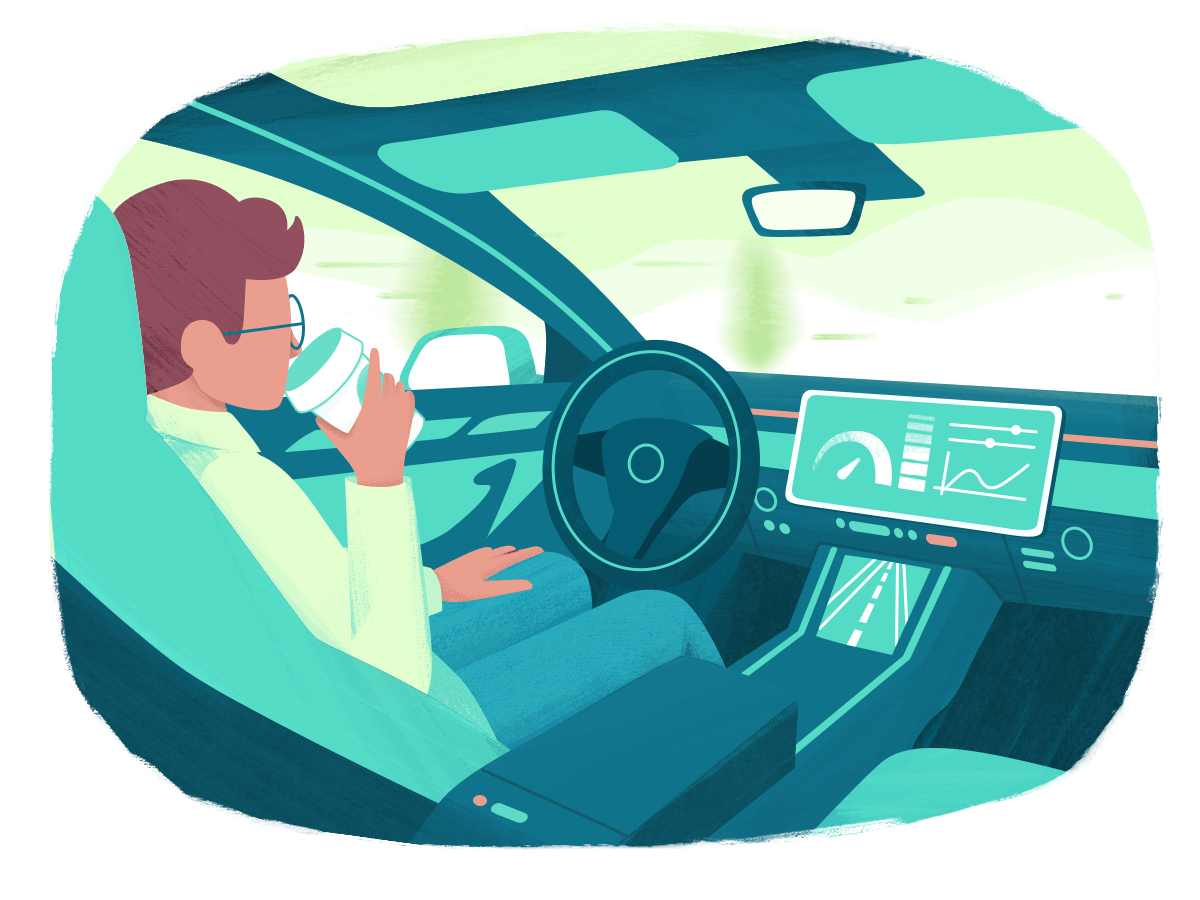
\includegraphics[width=0.50\linewidth]{AV}
	\caption{Concept visualization of autonomous driving. (source: \cite{AV})}
	\label{fig:AV}
\end{figure} 
\newpage

\section{Problem formulation and link with previous studies}
In order to identify specific comfort preferences of the driver that are quantified by parameters, the vehicle should be able to learn by demonstration. \cite{Kuderer2015a}\\
Despite that each driver has its own preferences, they are based on common comfort criteria where different trade-offs are made. For example, some drivers prefer a more aggressive driving style than others. This will manifest in a different set of parameters then the ones attained for a defensive driver for the same comfort criteria. The comfort criteria will later in this thesis be translated into an objective function where different weighting factors are used in order to quantify different comfort trade-offs made. In literature, this approach is called inverse optimal control or inverse reinforcement learning because it is learning the objective function for an optimal control problem.\\

In order to learn the weighting factors which can be used to distinguish different drivers, research about the common notion of comfort is necessary. Passenger surveys in public road transport about carsickness \cite{Turner1999} have identified lateral acceleration as the primarily responsible for motion sickness. It is explained that drive style is a main factor to influence the amount of sickness and it was found that sickness is higher when drivers drove with a higher average magnitude of fore-and-aft and lateral motion. These effects were far more significant than the effect of vertical vibrations. There is also a consensus reached about the contribution of continuous trajectories to the prevention of motion sickness and the natural feel of paths.\cite{Elbanhawi2015} This means that higher order kinematic variables like accelerations and jerks also should be considered when measuring comfort. Chapter \ref{cha:Literature_study} will give a more detailed description on the literature study conducted in order to investigate the state of the art comfort modelling. It will also discuss the theory of inverse reinforcement learning.\\

\section{Thesis objective and structure}
The goal of this thesis is to build further on research of learning by demonstration as explained in \cite{Kuderer2015a} and to refine this idea by making use of more realistic vehicle models. Concretely the thesis is focussed on the implementation and validation of an algorithm that learns weighting factors in a comfort objective function which can explain observed driver data.\\
The learning process is done offline. After the different weighting factors are identified, the learned objective can be used to plan paths which can be followed by an autonomous vehicle, making use of an online tracking MPC.\\

The data used as observations is generated by simulations where it is assumed that the vehicle is driving on an straight at a speed range between $80\frac{km}{hours}$ and $100\frac{km}{hours}$. The maneuver investigated is a lane change maneuver as can be seen in Figure \ref{fig:lane_change}. In order to generate data, the non-linear bicycle and a more realistic $15$ dof of freedom Amesim model are used.\\

\begin{figure}[htp]
	\centering
	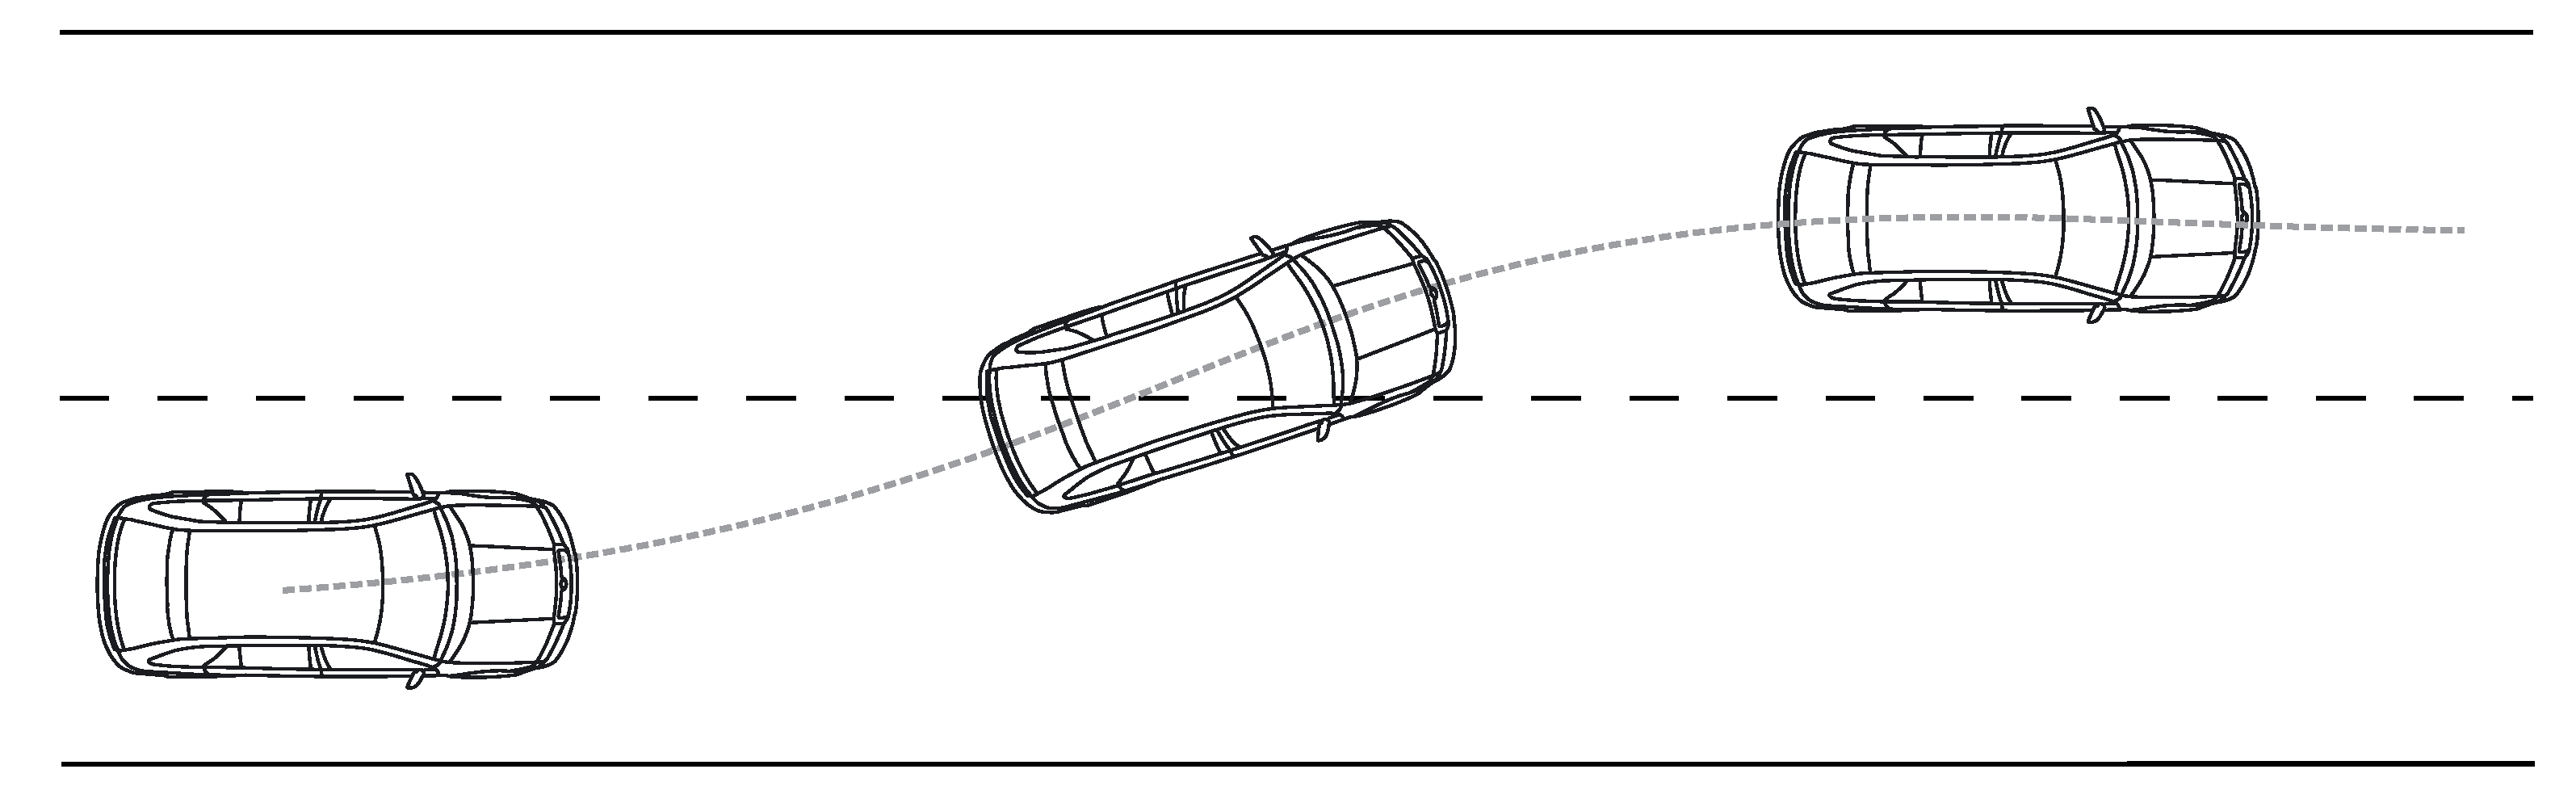
\includegraphics[width=0.8\textwidth]{lane_change.PNG}
	\caption{Example of a lane change which is the investigated maneuver in this thesis.}
	\label{fig:lane_change}
\end{figure}

The execution of this research was supported by "Siemens Digital Industries Software" located in Leuven which enabled a direct link with reality. Software was made available i.d. Simcenter Amesim.\\

The structure of the thesis is as follows. First, the reader is made acquainted with the optimal control concept in chapter \ref{cha:OCP}. The meaning is explained in section \ref{Optimal control problem (OCP)} and section \ref{s:MPC_e} gives an introduction to MPC. Next, chapter \ref{cha:Literature_study} discusses the state of the art modelling of comfort. This chapter is made out of 2 parts, section \ref{s:comfort_parameters} answers the question posed in section \ref{s:importance_topic}, explaining the meaning of comfort during driving. Section \ref{s:inverse re le} concerns a discussion on inverse reinforcement learning concept. Chapter \ref{cha:Learning_algorithm} gives insight in learning from ideal data. The non-linear bicycle model is discussed in section \ref{sec:Vehicle_models} whereafter the formulation of the learning algorithm follows in section \ref{s:learning_alg}. Next, ideal data generation is analysed and validated in section \ref{s:GD}. Subsequently, different methods for learning from multiple datasets are discussed and results were analysed in section \ref{s:ID_results}. In chapter \ref{cha:Tracking_MPC} the non-linear bicycle model will be substituted by a more complex $15$ degrees of freedom Amesim model. First the flow of the learning algorithm is discussed in section \ref{s:flow of the algorithm}. Next the developed tracking MPC needed, is presented in section \ref{s:tracking_mpc}. Section \ref{s:complex_learning_results} gives an overview of the learning results. 
In chapter \ref{cha:Enhancement} the theoretical concept of an enhanced weight factor update method is proposed. Finally, chapter \ref{cha:conclusion} gives an general conclusion of this thesis.\\

%The reader is first given an introduction in the optimal control concepts whereafter  Next the learning from ideal data is discussed and the learning algorithm is validated by finding back initial chosen weighting factors. After this, the non-linear bicycle model used is substituted by a more complex $15$ degrees of freedom Amesim model. 

%To be able to make the generated data of high quality an MPC approach with a 15 degree of freedom vehicle model is used. Also in the learning algorithm itself a three degree of freedom non-linear bicycle model is used in order to adequately capture the different kinematic signals e.g. jerks and accelerations. Further there were comparisons made of different methods to learn from multiple datasets. \\

% Therefore the objective of this research is to develop an algorithm based on inverse reinforcement learning which is able to learn driver specific experiences of comfort during a lane change, captured in weighting factors of an objective function. Learning is done by looking at observations performed by the human driver because the learned objective function is an approximation of the one used when the driver generates comfortable paths. Comfort features, which are integrated kinematic vehicle signals in a formulation so that they determine a notion of comfort, are used in order to quantify similarity between observed and learned vehicle paths. The contribution of this thesis is to implement the theoretical idea of feature based learning with practical relevant vehicle models e.g. a $15$ degrees of freedom Amesim model. When the comfort objective is identified, it can be embedded in a path planning formulation for autonomous driving.\\

%%% Local Variables: 
%%% mode: latex
%%% TeX-master: "thesis"
%%% End: 

\chapter{Comfort definition and modelling}
\label{cha:1}

Dan komt de vraag wat is comfort precies? Literatuur studie...
Waarnaar kan men kijken als men het over comfort heeft. 
Lane change bekeken om comfort te valideren --> zeg dat er geen iso standaarden aanwezig zijn.
Hoe wordt een bestuurder gemoddelleerd --> dit wordt gedaan door een kansverdeling.
Waarom is entropie nuttig om deze bestuurder te kunnen bekijken? Doe hier meer ondezoek over en verantwoord het gebruik hiervan. Conclusie komt af met comfort parameters die verder worden gebruikt als features.
Bij de uitleg van de features en waarom er versnelling en acceleratie wordt gebruikt, basseer ook op paper 7 van hoofdpaper

Wat wordt er in de literatuur al gebruikt om comfort te modelleren en geef een overzicht.

Leg uit hoe komt aan entropy distribution komt --> kan beroep doen op ref 2 en 20 van het hoofdrapport (both are assuming an exponential distribution) (IMPORTANT)


Dit is de reden voor het gebruik van de maximum entropie distributie: 
	To learn observed behavior, we aim to model the distribution
	that underlies the empirical sample trajectories.
	Following Abbeel and Ng [1], we aim to find a model that
	induces distributions that match, in expectation, the feature
	values fD of the empirical trajectories D, yielding
	Ep(x)[f (x)] = fD =
	1
	jDj
	X
	xk2D
	f (xk): (1)
	In general, however, there is not a unique distribution that
	matches the features. Ziebart et al. [24] resolve this ambiguity
	by applying the principle of maximum entropy [10], which
	states that the distribution with the highest entropy represents
	the given information best since it does not favor any
	particular outcome besides the observed constraints. (this is the least baised distribution)
	Modelling expected featueres by hybrid monte carlo method: https://reader.elsevier.com/reader/sd/pii/037026938791197X?token=71567B7640C402F2FF578E34E3BB7914CA14E4A1A29DE88D9534D96C9305E13DA52D0424FF1475A822FCE784725196D3
%	ref: C:\Users\t2vosx\OneDrive\Documenten\Leuven\Thesis\References2\Citations on main %paper\Learning to Predict Trajectories of Cooperatively Navigating Agents.pdf>

 	paper: Feature-based prediction of trajectories for socially compliant navigation
	which
	states that the distribution with the highest entropy represents
	the given information best since it does not favor any
	particular outcome besides the observed constraints.
	
%	• Weet dat exponentiële vorm oplossing is van boven staand optimizatie probleem. zie foto
%	--> volgt uit FONC --> oplossing moet (non convex) voldoen aan KKT conditions. Er zijn enkel maar equality constraints aanwezig --> primal feasibility en lagrange stationarity moeten voldaan worden --> LS wordt gecontroleerd drm van de Euler - lagrange vergelijking te gebruiken. 



\section{The First Topic of the Chapter}
First comes the introduction to this topic.


\subsection{An item}
Please don't abuse enumerations: short enumerations shouldn't use
``\verb|itemize|'' or ``\texttt{enumerate}'' environments.
So \emph{never write}: 
\begin{quote}
  The Eiffel tower has three floors:
  \begin{itemize}
  \item the first one;
  \item the second one;
  \item the third one.
  \end{itemize}
\end{quote}
But write:
\begin{quote}
  The Eiffel tower has three floors: the first one, the second one, and the
  third one.
\end{quote}

\section{A Second Topic}


\subsection{Another item}


\section{Conclusion}
The final section of the chapter gives an overview of the important results
of this chapter. This implies that the introductory chapter and the
concluding chapter don't need a conclusion.



%%% Local Variables: 
%%% mode: latex
%%% TeX-master: "thesis"
%%% End: 

\chapter{State of the art modelling of comfort}
\label{cha:Literature_study}
As discussed in the introduction, the goal of this thesis is to implement a method to capture personal experience of comfort during driving. This will be done by using an inverse reinforced learning where the weights in the objective function are learned from demonstration. To be able to do this, it is necessary that a literature study is done about how comfort is defined and to understand how to implement an inverse reinforced learning approach.\\

This chapter is structured as follows. First the question what comfort during driving means, will be answered in section \ref{s:comfort_parameters}. The second part (section \ref{s:inverse re le}) concerns a discussion of the inverse reinforcement learning concept used.

\section{What is comfort during driving?}
\label{s:comfort_parameters}
In the following US patent \cite{Daniel2018} the idea is to assess the amount of comfort by calculating a value for carsickness. This value is calculated by a weighted sum of sway motion, surge motion and heave motion of the vehicle. These motions are being directly calculated from the lateral acceleration, fore-aft acceleration and the vertical acceleration of the vehicle. \\

\begin{figure}[h!]
	\centering
	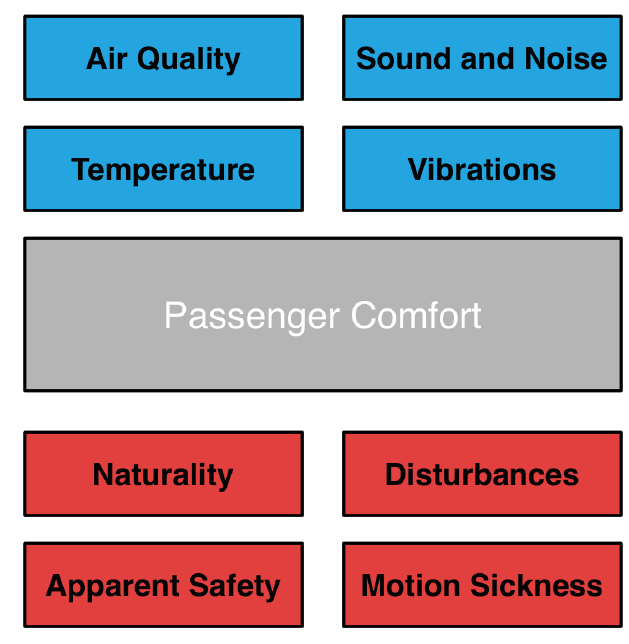
\includegraphics[width=0.48\textwidth]{comfort.PNG}
	\caption{Overview of comfort parameters in autonomous vehicle with old parameters (blue) and new ones (red).(Source: \cite{Elbanhawi2015})}
	\label{fig:Comfort}
\end{figure} 

%\begin{wrapfigure}[22]{L}{0.5\textwidth}
%	\begin{center}
%		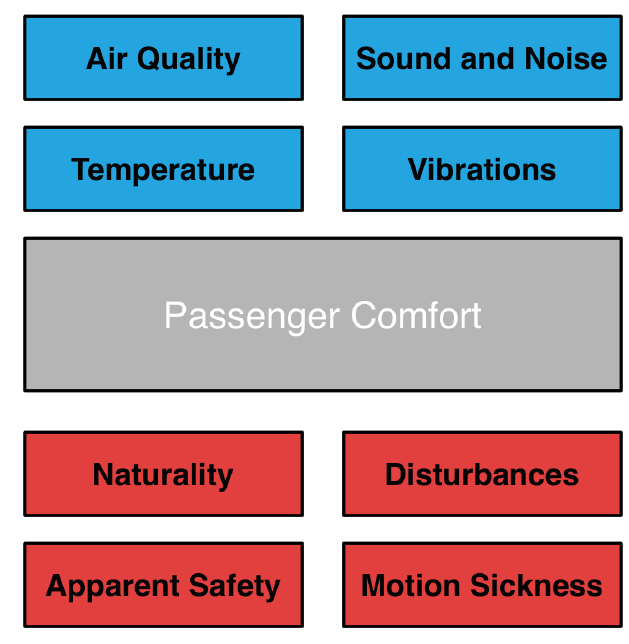
\includegraphics[width=0.48\textwidth]{comfort.PNG}
%	\end{center}
%	\caption{Overview of comfort parameters in autonomous vehicle with old parameters (blue) and new ones (red).(Source: \cite{Elbanhawi2015})}
%	\label{fig:Comfort}
%\end{wrapfigure}
In the paper 'Investigating ride comfort measures in autonomous cars' \cite{Elbanhawi2015}, it is explained that due to the introduction of autonomous vehicles there will be an other perception of comfort. Figure \ref{fig:Comfort} indicates in blue the claimed traditional comfort factors and in red the new ones that additionally have to be taken into account when driving in autonomous vehicles. Concretely this can be translated into the preference of smooth trajectories and low lateral motions when the roads are assumed to be sufficiently smooth. A hypotheses taken, is that motion sickness will be more prominent in autonomous driving due to the loss of control. Is is also argued that the distance to an obstacle is contributing to a comfortable feeling.\\

In 'Analysis of Driving Style Preference in Automated Driving' \cite{Bellem} three studies were completed in order to capture the definition of comfortable driving in autonomous vehicles.\\
During the first study, human drivers drove manually with their own driving style a set of maneuvers and in this data, there was sought after relevant metrics that could be used in defining comfortable driving. The results of this research was that accelerations play a key role in comfort but are not the only factor. \cite{Bellem}\\

\begin{quote}
	The different comfort metrics found were:
	\begin{itemize}
		\item longitudinal acceleration;
		\item lateral and longitudinal jerk;
		\item quickness of the maneuver;
		\item headway distance;
	\end{itemize}
\end{quote}

Quickness of the maneuver indicates that it is received as comfortable when the vehicle gives a good response and reaches the desired lateral displacement faster.
Additionally comfortable driving as assessed in \cite{Bellem}, can be summarized as  sufficiently smooth trajectories and keeping enough headway distance in order to have a feeling of control and safety. These results suggest that when an algorithm is evaluating comfort, a notion of the surrounding traffic should be present. It was found when the traffic density on the road is higher, the driver is more tolerant towards less smooth driving behaviour e.g. to be able to insert in a busy lane. In this case higher comfort can be attained if the driver has the feeling of a fast response of the vehicle, translating in early peaks of acceleration. Vertical vibrations come not in the scope when roads are assumed sufficiently smooth.\\

In a second study the main metrics that were found from study one are varied and combinations are rated by the use of a survey about the amount of comfort retrieved. "Out of this it followed that accelerations are again playing a key factor." \cite{Bellem} For lane changes it could be concluded that maneuvers with a small lateral acceleration and early perceivable onset were more comfortable.\\

That also jerk plays an important role in the attained amount of comfort, is confirmed by \cite{Gianna1996} where it is stated that: "Jerk has been shown to elicit a stronger influence on comfort than acceleration".


% In mijn maneuver wordt de kleine waardes van longitudinale snelheid en versnellingen gecompenseerd door de normalisatie waarden. Dus ookal zijn ze klein, krijgen toch een grote impact mee in het berekenen van een optimale oplossing. Daarin tegen kan er wel makkelijker voldaan worden aan het perfect voldoen van de longitudinale parameters in de lane change zonder het algemene resultaat veel te veranderen. De keuzen van de wegingsfactoren worden hierdoor minder significant en sensitiviteit wordt lager. --> als verschillende maneuvers worden gecombineerd zal dit de uniekheid van de gevonden wegingsfactoren opdrijven.

%Zie quotes van de slides!

\section{Inverse reinforcement learning}
\label{s:inverse re le}
Because every human has its own driving style it is a cumbersome task to tune these parameters for each individual in order to model a personal perception of comfort. In \cite{Powers} it is showed that manual tuned parameters will besides lead  to suboptimal solutions in comparison with from data learned parameters. Inverse reinforcement learning is the activity of learning an agents reward function from observations. \\

The goal of the learning algorithm explained in this thesis is to derive the parameters $\theta_j$ of different linearly combined comfort criteria $f_j$ combined in the cost function $J$. When the parameters are learned, the objective function $J$ will as best as possible explain the observed data. As the match with the observed data gets better during learning, it is assumed that $J$ is getting closer to the inner comfort function of the individual driver. However, it should be noted that the driver takes unknowingly a lot of comfort criteria into account and they are not all linearly relating as is suggested by Eq. (\ref{eq:1}). Therefore the comfort cost function in Eq. (\ref{eq:1}), will always be an approximation of reality. Although as discussed in \cite{Kuderer2015a}, it is possible to capture the magnitude of the main drivers that contribute to the comfort experienced by the users.\\

\begin{equation}\label{eq:1}
	J = \sum_{j=1}^{Z}\theta_j\cdot f_j	
\end{equation}

%"Inverse optimal control, also known as inverse reinforcement learning, is the problem of recovering an unknown reward function in a Markov decision process from expert demonstrations of the optimal policy." \cite{Levine2012} In contrary what this classic definition, the approach followed by \cite{Kuderer2015a} is not modelling teh

In order to create a generative model that creates vehicle paths $\bm{r}_i$ with equivalent kinematic characteristics as the path that was observed $\tilde{\bm{r}_i}$, a feature-based inverse reinforcement learning is applied. \cite{Kuderer2015a,Abbeel2004} With $i \in [1 ... m]$ and $m$ the amount of observed trajectories. A feature is encoding relevant kinematic properties onto a scalar value and the difference between the demonstrated and calculated features give a clear indication about the similarity of the kinematic signals i.e. displacement,velocity, acceleration and jerk. \\

\subsection{Feature based reinforcement learning}
A feature value maps a signal onto a scalar and encapsulates a comfort criteria. The higher the scalar value the more discomfort is experienced by the driver. An example is given by Eq. (\ref{eq:3}) that measures the amount of accelerations in a maneuver.

\begin{equation}\label{eq:3}
f_j:\bm{r}\xrightarrow{}f_j(\bm{r})=\int_{0}^{T}a_x(t)^{2}+a_y(t)^{2} dt
\end{equation}
The different feature values are collected in a feature vector $\bm{F} \in \mathbb{R}^Z$ with on its entries the different feature values $f_j$.
The path that the centre of gravity of the vehicle is following can be represented by Eq. (\ref{eq:4}).
\begin{equation}\label{eq:4}
\bm{r}:t \xrightarrow{}\bm{r}(t) =  \bigl( \begin{smallmatrix} x(t)\\ y(t) \end{smallmatrix}\bigr)
\end{equation}

The human driver is not a deterministic agent and is modelled by a stochastic distribution $p(\bm{r}|\bm{\theta})$. For certain weights $\bm{\theta} \in \mathbb{R}^Z$ a path $\bm{r}$ is produced as being a sample of a stochastic distribution. The distribution that is chosen for this is the distribution of maximum entropy Eq. (\ref{eq:entropy}). \cite{Ziebart2008}. 
The distribution with the highest entropy represents the given information best since it does not favour any particular outcome besides the observed constraints. \cite{Abbeel2004}
	
\begin{equation}\label{eq:entropy}
	p(\bm{r}|\bm{\theta}) = exp(-\bm{\theta}^T\cdot \bm{F}(\bm{r}))
\end{equation}
Equation \ref{eq:entropy} can be interpreted as a cost function $\bm{\theta}^T\bm{F}(\bm{r})$ where agents are exponentially more likely to select trajectories with lower cost. \cite{Kuderer2015a}
The observed feature vector $\tilde{\bm{F}} \in \mathbb{R}^Z$ has on its entries the different feature values $\tilde{f_j}$. 

%The averaged observed feature vector is $\tilde{\bm{F}}_{av} = \frac{1}{m}\sum_{j=1}^{m}\tilde{\bm{F}_j}$.\\

In order to explain the observed feature vector, the weights $\bm{\theta}$ need to be found that match the expected features vector $\bm{F}(\bm{r}_{expected})$ with $\tilde{\bm{F}}$. $\bm{r}_{expected}$ is defined as $ E(p(\bm{r}|\bm{\theta}))$. To go towards a match with the observed feature vector, a gradient descent method can be used with an estimation of the gradient $\pdv{\bm{F}_{diff}}{\bm{\theta}}$ by $\bm{F}_{obs} - \bm{F}(\bm{r}_{expected})$ and with $\bm{F}_{diff}$ the difference between the feature vectors. \cite{Ziebart2008, Kretzschmar2014}. Only the sign of the gradient is used and there are two directions for every weight update: increase or decrease. Therefore an intuitive explanation exist for using $\bm{F}_{obs} - \bm{F}(\bm{r}_{expected})$ as estimation for the gradient. The weight is increased when the expected feature is higher than the observed one, which means that the associated comfort feature will be punished more severely during the generation of $\bm{r}_{expected}$ in the next iterate. Consequently, the weight will be decreased when the expected feature is lower than the observed one. \cite{Kuderer2015a} Equation \ref{eq:5} summarizes the gradient descent method with $\alpha$ the step size taken in the direction of descent.
\begin{equation}\label{eq:5}
	\bm{\theta}^{k+1} = \bm{\theta}^{k} - \alpha \pdv{\bm{F}_{diff}}{\bm{\theta}}^k 
\end{equation}

When $\bm{\theta}_{optimal}$ is found the gradient is minimized and the feature vectors will match as closely as possible. But the problem remains how to retrieve $\bm{F}(\bm{r}_{expected})$. In order to calculate $\bm{F}(\bm{r}_{expected})$ a Hamiltonian Markov chain
Monte Carlo stochastic distribution sampling method was used in \cite{Kretzschmar2014}. In \cite{Kuderer2015a} a simplified and less calculation demanding approach is proposed, where it is assumed that the expected path is also the one that is been assessed as the most comfortable by the human driver. The path that is perceived as the most comfortable can be estimated by minimizing Eq. (\ref{eq:1}) for certain weights. Equation \ref{eq:6} summarizes the method proposed by \cite{Kuderer2015a}.
\newcommand{\argmax}{argmax}
\newcommand{\argmin}{argmin}
\begin{subequations}
	\label{eq:6}
\begin{equation}
	\bm{r}_{expected} = \underset{\bm{r}}{\argmax} \hspace{1mm} p(\bm{r}|\bm{\theta}) = \underset{\bm{r}}{\argmin} \hspace{1mm}  \bm{\theta}^T\cdot \bm{F}(\bm{r})
\end{equation}
\begin{equation}\label{eq:new}
	\pdv{\bm{F}_{diff}}{\bm{\theta}} = \bm{F}_{obs} - \bm{F}(\bm{r}_{expected})
\end{equation}
\end{subequations}

%\DeclareMathOperator*{\argmin}{argmin}

\subsection{RPROP algorithm}\label{s:RPROP}
From \cite{Panos_opti} it is known that not every step size of the gradient is leading to convergence towards a minimum. When the step size is too small it will take a long time to convergence. However when it is chosen too big, cycling behaviour between limit points can occur. In order to avoid this kind of unwanted behaviour a  method is needed in order to change the step size taken during the course of the algorithm. For this the Resilient backpropagation algorithm (RPROP) \cite{RPROP} is used as it was first proposed by Martin Riedmiller and Heinrich Braun in 1993.\\

The main advantage when using RPROP is that the size of the gradient is not blurring the update value of the weights. The update value $\Delta u$ is solely dependent on the sign of the current gradient, the sign of the gradient in the previous iteration and the update value in the previous iteration. The three possible cases for the update value during iteration $t$ is given by: 

\begin{equation}\label{eq:7}
	\Delta u^t_i =
	\begin{Bmatrix}
		 \eta^+ \cdot \Delta u^{t-1}_i, & if \hspace{1 mm} \pdv{f_i}{\theta_i}^t \cdot \pdv{f_i}{\theta_i}^{t-1} > 0 \\
		 \eta^- \cdot \Delta u^{t-1}_i, & if \hspace{1 mm} \pdv{f_i}{\theta_i}^t \cdot \pdv{f_i}{\theta_i}^{t-1} < 0 \\
		  \Delta u^{t-1}_i, & if \hspace{1 mm} \pdv{f_i}{\theta_i}^t \cdot \pdv{f_i}{\theta_i}^{t-1} = 0 \\
	\end{Bmatrix}
\end{equation}
\begin{equation}\label{eq:9}
0 <\eta^-<1<\eta^+
\end{equation}

When the update value of the weight is determined it is applied in the direction of steepest descent which equals the opposite direction of the current gradient. 

\begin{equation}\label{eq:8}
\Delta \theta^t_i =
\begin{Bmatrix}
	-\Delta u^t_i, & if \hspace{1 mm} \pdv{f_i}{\theta_i}^t > 0 \\
	+ \Delta u^t_i, & if \hspace{1 mm} \pdv{f_i}{\theta_i}^t < 0 \\
	0, & else 
\end{Bmatrix}
\end{equation}
Exception on Eq. (\ref{eq:8}):

\begin{equation}\label{eq:10}
	\Delta \theta^t_i = -\Delta \theta^{t-1}_i, \hspace{1mm} if \hspace{1mm} \pdv{f_i}{\theta_i}^t \cdot \pdv{f_i}{\theta_i}^{t-1} < 0
\end{equation}



and with $\theta_i^{t+1} = \theta_i^{t} + \Delta \theta^t_i$, $i \in \mathbb{N}_{[1\cdots Z]}$ and $t \in \mathbb{N}_{[1 \cdots \mathbb{\tau}]}$ the amount of iterations. Every time the partial derivative $\pdv{f_i}{\theta_i}^t$ of the corresponding weight $\theta_i^t$ changes its sign, it is assumed that the last update was too big and the local minimum was passed. In Eq. (\ref{eq:7}) the step size is then reduced and in order to go back to the previous situation the update of the weight is done as indicated by Eq. (\ref{eq:10}). In order to not again decrease the update value when going back to the previous situation where the gradient will again change it's sign,  $\pdv{f_i}{\theta_i}^{t}$ is set to zero.\\
If the derivative retains its sign with respect to the previous iteration, the update value is slightly increased in order to accelerate convergence in shallow regions." \cite{RPROP} Parameters set by the user are $\Delta u^0_i,\Delta u^{max}_i,\Delta u^{min}_i, \eta^+$ and $\eta^-$. In this thesis following values were chosen: $\Delta u^0_i = 0.1$, $\Delta u^{max}_i=1.0$, $\Delta u^{min}_i=10^{-7}$, $\eta^+ = 1.2$ and $\eta^- = 0.5$.

%e the assumption of calculating most likely path --> features expected = f(r_exp) instead of sampling as is done in this paper.
%(Hamiltonian Markov chain Monte Carlo methods = very computation expensive)
%



%When the averaged observed feature vector $F$
%
%In order to be able to explain the observed trajectory
%
% Firstly he is generating observed paths that are a sample of a distribution and secondly he is minimizing its own comfort cost function.
%
% 
%The exponential distribution is giving a higher chance to produce paths that have a low feature value associated  with a high weight factor. This means that the more influence a feature value has on the total amount of comfort (higher weight), how less likely it becomes that the driver will produce a certain path that will trigger a high value of the concerned feature value. 
%
%If you maximize the probability you get the most likely expected path for the chosen weights.  This can be translated in the assumption that the driver is most likely to produce a path that will be experienced as comfortable as possible by himself. The assumption that the driver is optimizing its own comfort cost function is an assumption on top of assuming that the observed path is a sample of an exponential distribution with certain weight factors. 
%
%The goal of the learning process is to learn the model parameters (weight factors) of the driver from their observed driving style. It is assumed that the driver can be explained by a probability distribution and that it produces paths that minimize a comfort cost function. When the comfort model of the driver is learned, it can be further used in general situations. This is done by implementing the user specific notion of comfort in the motion planning algorithm of a model predictive control planning application.
%
%The learned model should produce trajectories that are similar in order of comfort as experienced by the driver. This is a logical consequence because the model is derived from the observed data. The difference between the features of the observed and generated paths quantify the similarity and at convergence of the learning algorithm, the feature values are as close as possible. As close as possible should be taken with a grain of salt though. This can be explained by making a comparison between the curvature and the jerk where curvature is in order of 10^-5 and jerk is in order of 10^2. This means that a difference of 1 has a far more bigger impact on curvature than on jerk and normalization is necessary. Normalization is done by dividing the calculated features by their corresponding observed feature value in order to make it dimensionless.  This means that the optimization should be done without fixing time! The difference in feature values is the driving factor and this will indirect specify also the time of the lane change.
%
%Learning a model implies finding the best suitable values of the tunable parameters which are in this case the weight factors. To summarize, the goal of the learning algorithm is to find the weight factors which give the smallest difference between the feature values of the observed path and the feature values of the calculated path, which is the path that minimizes the linear comfort cost function. The calculated path is generated by the minimization of the comfort cost because minimizing the comfort cost function is equal to maximizing the exponential distribution and the resulting path is equal to the most likely generated path for certain weight factors. The most likely generated path is compared with the observed one. With this it is indirectly assumed that the observed paths are generated by a human driver that is minimizing its own unknow comfort cost function. It will be clear from the validation in chapter \ref{} if this assumption holds. From [hoofdrapport] it is assumed that this approximation is suitable in the context of learning individual driving styles on highways.  Two assumptions apply on the human driver. Firstly he is generating observed paths that are a sample of a distribution and secondly he is minimizing its own comfort cost function. It should be noted that in practice instead of using personal data also data form an expert driver can be made available to the user. This to avoid bad autonomous behavior as a result of an inexperienced human driver.
%
%
%Note that the features of the path that are obtained by minimizing the comfort cost function should be possible to converge to the features of the observed path. The driver that is producing the observed path is assumed to maximize its personal comfort when generating the observation data which means that the most personal comfort is attained when the difference between the feature values of the observed and calculated paths are small. (this should be normalized) 
%


\section{Conclusion}
In order to find parameters of driving comfort that will be used as comfort criteria, a literature study was conducted which was mainly questionnaire based. The results were that in order to be able to evaluate comfort, higher order kinematic variables like accelerations and jerks must be considered. These variables are important to acquire a smooth vehicle path and to give a continuous and natural feeling when driving. Also should the quickness of the maneuver and the feeling of driving save be taken into account. Therefore comfort is naturally be influenced by the environment of the vehicle. It was found that when more traffic is present, a higher tolerance for less smooth trajectories is granted. Finally it was explained that if the goal of the maneuver was more rapidly completed this influenced the amount of comfort in a positive way.\\

In the second part of the literature study the concept of inverse reinforcement learning was clarified and it was explained that it is the process of identifying the unknown objective of the human driver. Next there has been looked into feature based learning and a practical method was found in order to retrieve $\bm{\theta}_{opti}$ making use of gradient descent. After this the RPROP algorithm was introduced that will be used to update the weights while making use of the gradient descent method in order to match expected feature values with the observed ones.

\newpage


%\section{bekijk hiervoor de andere approaches - to be read further}
%
%\subsection{Machine learning approach}
%\subsection{paper brecht approach}

%Dan komt de vraag wat is comfort precies? Literatuur studie...
%Waarnaar kan men kijken als men het over comfort heeft. 
%Lane change bekeken om comfort te valideren --> zeg dat er geen iso standaarden aanwezig zijn.
%Hoe wordt een bestuurder gemoddelleerd --> dit wordt gedaan door een kansverdeling.
%Waarom is entropie nuttig om deze bestuurder te kunnen bekijken? Doe hier meer ondezoek over en verantwoord het gebruik hiervan. Conclusie komt af met comfort parameters die verder worden gebruikt als features.
%Bij de uitleg van de features en waarom er versnelling en acceleratie wordt gebruikt, basseer ook op paper 7 van hoofdpaper--> geen acces
%
%Wat wordt er in de literatuur al gebruikt om comfort te modelleren en geef een overzicht.
%
%Leg uit hoe komt aan entropy distribution komt --> kan beroep doen op ref 2 en 20 van het hoofdrapport (both are assuming an exponential distribution) (IMPORTANT) --> literatuur study niet te uitgebreid maken...
%
%Check uitgebreide samenvatting van hoofdpaper op oneNote.
%
%Dit is de reden voor het gebruik van de maximum entropie distributie: 
%	To learn observed behavior, we aim to model the distribution
%	that underlies the empirical sample trajectories.
%	Following Abbeel and Ng [1], we aim to find a model that
%	induces distributions that match, in expectation, the feature
%	values fD of the empirical trajectories D, yielding
%	Ep(x)[f (x)] = fD =
%	1
%	jDj
%	X
%	xk2D
%	f (xk): (1)
%	In general, however, there is not a unique distribution that
%	matches the features. Ziebart et al. [24] resolve this ambiguity
%	by applying the principle of maximum entropy [10], which
%	states that the distribution with the highest entropy represents
%	the given information best since it does not favor any
%	particular outcome besides the observed constraints. (this is the least baised distribution)
%	Modelling expected featueres by hybrid monte carlo method: https://reader.elsevier.com/reader/sd/pii/037026938791197X?token=71567B7640C402F2FF578E34E3BB7914CA14E4A1A29DE88D9534D96C9305E13DA52D0424FF1475A822FCE784725196D3
%%	ref: C:\Users\t2vosx\OneDrive\Documenten\Leuven\Thesis\References2\Citations on main %paper\Learning to Predict Trajectories of Cooperatively Navigating Agents.pdf>
%
% 	paper: Feature-based prediction of trajectories for socially compliant navigation
%	which
%	states that the distribution with the highest entropy represents
%	the given information best since it does not favor any
%	particular outcome besides the observed constraints.
	
%	• Weet dat exponentiële vorm oplossing is van boven staand optimizatie probleem. zie foto
%	--> volgt uit FONC --> oplossing moet (non convex) voldoen aan KKT conditions. Er zijn enkel maar equality constraints aanwezig --> primal feasibility en lagrange stationarity moeten voldaan worden --> LS wordt gecontroleerd drm van de Euler - lagrange vergelijking te gebruiken. 


%%% Local Variables: 
%%% mode: latex
%%% TeX-master: "thesis"
%%% End: 

\chapter{Learning from ideal data}
\label{cha:Learning_algorithm}

This chapter is focussing on the implementation of the inverse reinforcement learning idea that is used to learn the different weights in the comfort cost function $\bm{\theta}^T\bm{F}(\bm{r})$ as
explained in chapter \ref{cha:Literature_study}. The use of ideal data is assumed which means that vehicle model mismatch is avoided by using the same model for learning the weights and generating data. Thereby is the approximation that comfort of a driver is modelled by a linear relation of features exactly for-filled. Data is generated by choosing a set of weights and generating kinematic vehicle signals by making use of the minimization seen in Eq.(\ref{eq:6}). A validation of the developed learning algorithm is done when the chosen weights used in generating the data are found back.\\

First the non-linear bicycle model and the used parameters is explained. There is chosen for a bicycle model because this can model the dynamics sufficiently during a comfortable lane change maneuver and the calculation cost stays affordable. The model makes abstraction of suspension dynamics i.e. neglects rolling and pitching and the centre of gravity is fixed during driving. \cite{Yankov}  Further on, the concretely used algorithm is discussed. After that a detailed discussion is given about the simulations done.\\
It is worth noting that the learning process discussed, concerns an offline optimization which allows for higher calculations loads because of the absence of pushing real time constraints.

\begin{figure}[h!]
	\centering
	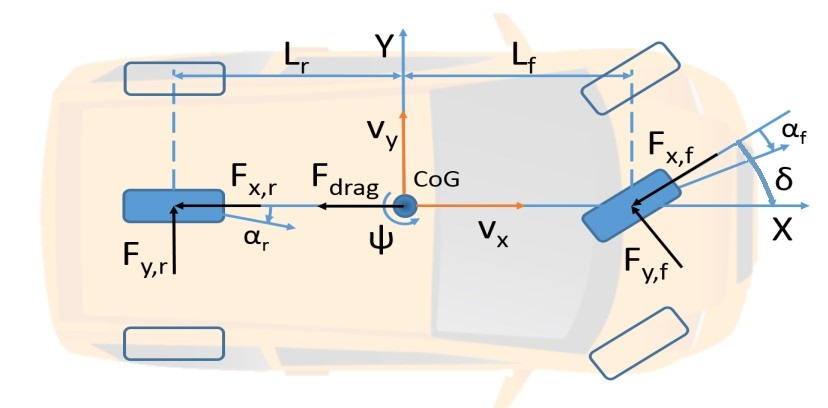
\includegraphics[width=0.5\textwidth]{Bicycle_model_paper.png}
	\caption{Non-linear bicycle model (Source: \cite{TongDuySon2019}).}
	\label{fig:bicycle_model}
\end{figure}
\section{Non-linear bicycle model}\label{sec:Vehicle_models}
The free body diagram of the non-linear bicycle model can be seen in figure \ref{fig:bicycle_model}.



Two variants of this model are discussed which are differentiated by the smoothness of the controls that are used. 
\begin{enumerate}
	\item	Model has 6 states and 2 controls: 
	\begin{equation}\label{eq:bicycle_model1}
	\centering
	\bm{X} = 
	\begin{bmatrix}
	x & y & v_x & v_y & \psi & \dot{\psi}
	\end{bmatrix}^{T}
	\; and \; \bm{U} = 
	\begin{bmatrix}
	t_r & \delta
	\end{bmatrix}^{T}
	\end{equation}
	
	\item Model has 10 states and 2 controls:
	\begin{equation}\label{eq:bicycle_model2}
	\centering
	\bm{X} = 
	\begin{bmatrix}
	x & y & v_x & v_y & \psi & \dot{\psi} & t_r & \delta & a_x & a_y
	\end{bmatrix}^{T}
	\; and \; \bm{U} = 
	\begin{bmatrix}
	\dot{t_r} & \dot{\delta}
	\end{bmatrix}^{T}
	\end{equation}
\end{enumerate}


$x$ and $y$ in the above formulation are the position of the centre of gravity of the vehicle in the global coordinate system. $v_x$ and $v_y$ are the vehicle velocities in the local vehicle frame. $\psi$ is the vehicle yaw angle and $\dot{\psi}$ the yaw rate.  The control vector of Eq. (\ref{eq:bicycle_model1}) consists of the throttle $t_r$ and the angle of the front wheel $\delta$. In the more extended bicycle model Eq. (\ref{eq:bicycle_model2}) throttle and front wheel angle serve as states. $a_x$ and $a_y$ are the total accelerations of the centre of gravity in the local vehicle frame. The inputs in this second formulation are the first order derivatives of throttle and front wheel angle.\\

The equations of motion derived and checked in literature \cite{TongDuySon2019} are\footnote{Appendix \ref{app:A} shows the complete jerk equations $j_x$ and $j_y$.} :
\begin{equation}\label{eq:bicycle_model_eqmotion}
\begin{aligned}
\dot{x} = v_x cos(\psi) - v_y sin(\psi)\\
\dot{y} = v_x sin(\psi) + v_y cos(\psi)\\
m \dot{v}_x = F_{x,f} cos(\delta) - F_{y,f} sin(\delta) + F_{x,r} - F_{drag} + m v_y \dot{\psi}\\
m \dot{v}_y = F_{x,f} sin(\delta) + F_{y,f} cos(\delta) + F_{y,r} - m v_x \dot{\psi}\\
\dot{\psi} = \dot{\psi}\\
I_z \ddot{\psi} = L_f (F_{y,f} cos(\delta) + F_{x,f} sin(\delta)) - L_r F_{y,r}\\
\dot{t_r} = \dot{t_r}\\
\dot{\delta} = \dot{\delta}\\
a_{tx} = \dot{v}_x\\
a_{nx} = -v_y\dot{\psi}\\
a_{ty} = \dot{v}_y\\
a_{ny} = v_x\dot{\psi}\\
j_x = \dot{a}_{tx} + \dot{a}_{nx}\\
j_y = \dot{a}_{ty} + \dot{a}_{ny}
\end{aligned}
\end{equation}
\newpage
The drag force is calculated as:
\begin{equation}\label{eq:bicycle_Fdrag}
\begin{aligned}
F_{drag} = C_{r0} + C_{r1} v_x^2
\end{aligned}
\end{equation}
with $C_{r0}$ the roll resistance and $C_{r1}$ the air drag contributions.\\

To calculate the tyre forces, a linear tyre model is used instead of a more complex non-linear model e.g. Pacejka tyre model. The longitudinal tyre forces are calculated as:
\begin{equation}\label{eq:bicycle_Fx}
\begin{aligned}
F_{x,f} = \frac{t_r T_{max}}{2 R_w}\\
F_{x,r} = F_{x, f}
\end{aligned}
\end{equation}

$R_w$ is the wheel radius and $T_{max}$ a measure for the maximum torque the engine is able to supply. Because $F_{x,r} = F_{x, f}$ the longitudinal forces that are induced by the engine are equally distributed between front and rear axle (division by 2 in above equations). The coefficient $t_r$ is the normalised amount of throttle that can be applied and has a value between -1 and 1 (negative for braking). In the bicycle model it is assumed that braking behaves the same as giving a negative amount of throttle.
The lateral tyre forces are calculated based on the tyre slip angles $\alpha_f$ and $\alpha_r$:
\begin{equation}\label{eq:bicycle_slipangle}
\begin{aligned}
\alpha_f = -atan(\frac{\dot{\psi} L_f + v_y}{v_x}) + \delta\\
\alpha_r = atan(\frac{\dot{\psi} L_r - v_y}{v_x})
\end{aligned}
\end{equation}
resulting in:
\begin{equation}\label{eq:bicycle_Fy}
\begin{aligned}
F_{y,f} = 2 K_f \alpha_f\\
F_{y,r} = 2 K_r \alpha_r
\end{aligned}
\end{equation}\\
The use of this linearised lateral tyre model is valid for small lateral accelerations ($a_y <= 4 m/s^2$) and slip angles ($\alpha <= 5^o$) \cite{TongDuySon2019}. It is acceptable to use this approximate model in this thesis as the goal is to learn a comfortable and thus smooth lane change manoeuvre. These constraints will be checked during section \ref{s:GD_val}.\\

The vehicle model parameters used are given in table \ref{table:vehicel_model_param}. These numbers were provide by Siemens Digital Industries Software. The $Gsteerfactor$ approximates linearly the relation between the front wheel angle and the steer wheel angle turned by the driver: $\delta = \frac{\delta_s}{Gs}$.  

\begin{table}[h]
	\centering
	\begin{tabular}{|p{5cm}|p{2cm}|}
		\hline
		\textbf{Parameter} & \textbf{Value}\\ \hline		
		Vehicle mass $m$ [kg] & 1430\\ \hline
		Moment of inertia $I_z$ [$kgm^2$] & 1300\\ \hline
		Front axle distance $L_f$ [m] & 1.056\\ \hline
		Rear axle distance $L_r$ [m] & 1.344\\ \hline
		Roll resistance coefficient $C_{r0}$ [N] & 0.6\\ \hline
		Air drag coefficient $C_{r1}$ [$\frac{Ns^2}{m^2}$] & 0.1\\ \hline
		Engine torque limit $T_{max}$ [Nm] & 584\\ \hline
		Wheel radius $R_w$ [m] & 0.292\\ \hline
		Lateral front tyre stiffness $K_{f}$ [N] & 41850.85\\ \hline
		Lateral rear tyre stiffness $K_{r}$ [N] & 51175.78\\ \hline
		Gsteerfactor $Gs$ [-] &16.96 \\ \hline
		
	\end{tabular}
	\caption{Used vehicle model parameters.}
	\label{table:vehicel_model_param}
\end{table}
\newpage
\section{Formulation of the algorithm} 
\label{s:learning_alg}
The goal of the learning algorithm is to learn the weights $\bm{\theta}$ in the pre-defined comfort objective function: $\bm{\theta}^T\bm{F}(\bm{r})$. The features that are the entries of the feature vector $\bm{F}(\bm{r})$ capture a notion of comfort felled by the driver. Based on the literature study displayed in Chapter \ref{cha:Literature_study} and on paper \cite{Kuderer2015a}, the amount of discomfort can be modelled by the features discussed in section \ref{s:obj} during the timespan $T$ of the maneuver. The scenario of a lane change on a highway is modelled. The time horizon about what the minimization of the comfort objective function is done, itself is also an optimization variable  $T$. The simulations done in this thesis are performed on a notebook provided by Siemens with Intel Core i7-7920HQ CPU @ 3.10GHz and 32 GB of RAM memory.\\


\subsection{Flow of the algorithm}
%The goal of the learning algorithm is to output weights that when applied in the objective $\bm{\theta}^T\bm{F}(\bm{r})$, generate feature vector  $\bm{F(\bm{r})}$ that are the best possible fit with the observed feature vector. Without a vehicle mismatch a match of feature values will directly induce a good match of the kinematic signals as is extensively discussed in section \ref{s:ID_results}. 

%This means that similarity between the observed path and the one that follows from minimizing the objective $\bm{\theta}^T\bm{F}(\bm{r})$ for chosen weights, is quantified by the difference between the feature values of the observed path and the obtained one. 

As has been discussed in chapter \ref{cha:Literature_study},  $\bm{\theta}_{opti}$ gives the best possible fit between $\bm{F}(\bm{r}_{expected})$ and $\bm{\tilde{F}(\bm{r})}$.
Without a vehicle mismatch, a match of feature values will induce a good match of the kinematic signals as is discussed in section \ref{s:ID_results}.
The flow of a single dataset learning algorithm can be seen in Figure \ref{fig:basic learning}.\\

%The path that is expected to be produced by the driver is the path that is felt as the most comfortable and equals $\bm{r}_{expected} =  \underset{\bm{r}}{\argmin} \hspace{1mm}  \bm{\theta}^T\cdot \bm{F}(\bm{r})$.\\

The learning is started by guessing a set of weights e.g. all equal to one. Equation \ref{eq:6} is minimized to generate an expected path for them. From this features can be retrieved by using the definition discussed in \ref{s:obj}. Afterwards, the relative features $f_{rel,i}$ are calculated by dividing the expected features by the observed ones. A perfect match is acquired when the division equals one and the learning algorithm is terminated. The tolerance on convergence towards one, is chosen during this chapter equal to $10^{-3}$.

\begin{figure}[h!]
	\centering
	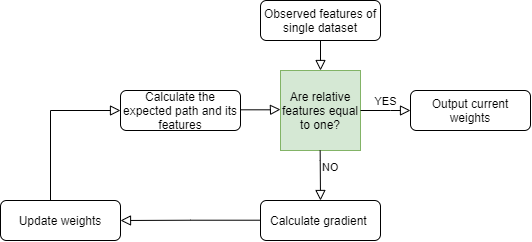
\includegraphics[width=1.0\textwidth]{basic_learning.png}
	\caption{Basic flow of the reinforced learning algorithm.}
	\label{fig:basic learning}
\end{figure}

  
While no convergence takes place the weights are updated, making use of the estimation of the gradient and the RPROP algorithm explained in Chapter \ref{cha:Literature_study}. The new weights are used to calculate a new expected path which will result in different expected feature values $\bm{F}(\bm{r}_{expected})$.  Next a more detailed description of the calculation of the expected path is given by Eq. (\ref{opt:basic_opti_w}) which uses as vehicle model Eq. (\ref{eq:bicycle_model2}). \\

%In order to apply the RPROP method only the sign of the gradient is used which means that the size of the gradient is decoupled from the update value of the weights. The estimate of the gradient is given by $\pdv{\bm{F}}{\bm{\theta}} = \bm{F}_{obs} - \bm{F}(\bm{r}_{expected})$  and the update of the weight is achieved by applying the gradient method according to $\bm{\theta}^{k+1} = \bm{\theta}^{k} - |\Delta \theta^{k}|sign( \pdv{\bm{F}}{\bm{\theta}}^k )$ where $\Delta \theta^{k}$ is calculated according section \ref{s:RPROP}. If follows that the weight $\theta_i$ is decreased if $f_{obs,i}>f_{i}(\bm{r_{exptected}})$ and increased when $f_{obs,i}<f_{i}(\bm{r}_{exptected})$.

\begin{equation}\label{opt:basic_opti_w}
\begin{aligned}
\min_{\bm{X}(.),\bm{U}(.), T} \quad &  \bm{\theta}^T\bm{F}(\bm{X},\bm{U}, T) \\
\textrm{s.t.} \quad & \bm{X}^{k+1} = I(\bm{X}^{k}, \bm{U}^{k}) & k = [0,\cdots, N-1]\\
& \bm{X}^{0}[1:8]= \bm{X}_{intitial} \\
& T \leq T_{limit}\\
& \bm{F}(\bm{X}^{k}) \geq 0	& k = [0,\cdots, N]\\
& \bm{H}(\bm{X}^{k}) = 0	& k = [0,\cdots, N]\\
& \bm{X}^{k}\in \mathbb{R}^{10\times 1}  & k = [0,\cdots, N]\\
& \bm{U}^{k}\in \mathbb{R}^{2\times 1} \hspace{3 mm} & k = [0,\cdots, N-1]\\
& T \in \mathbb{R},\hspace{3 mm} N \in \mathbb{N}
\end{aligned}
\end{equation}

Where $\bm{X} \in \mathbb{R}^{10\times N+1}$ and $\bm{U}\in \mathbb{R}^{2\times N}$ contain respectively the states and controls of Eq.(\ref{eq:bicycle_model2}) during the maneuver. The time of the maneuver is represented as $T$. In order to discretize time, a multiple shooting approach is adopted as is explained in section \ref{s:time_dis}. The amount of integration intervals $N$ is chosen equal to $1000$ and determines the  amount of control applied to go from the initial state towards the end state. 
Inside the function $I$ the Runge-Kutta time integration method is embedded in order to connect different states over time when a certain control is applied for $\Delta T$. Here the equations of motion Eq. (\ref{eq:bicycle_model_eqmotion}) are inputted in the optimization because derivatives of the vehicle states are needed. The time discretization used can be categorized as a direct method and because a multiple shooting approach is used at every time instance a new set of state optimization variables is introduced as is explained in section \ref{s:time_dis}. The path constrain vector $\bm{F}$ demarcates together with the equality constraint vector $\bm{H}$, the feasible space of the solutions for $\bm{X}$ and $\bm{U}$. An overview of the constraints used, is given by Eq. (\ref{eq:F}) and Eq. (\ref{eq:H}).

\begin{equation}\label{eq:F}
\bm{F} =
\begin{Bmatrix}
-\frac{Width\hspace{1mm}Lane}{2} \leq y^k \leq \frac{3\cdot Width\hspace{1mm}Lane}{2}, & k = [0,\cdots, N] \\
0 \leq x^k, & k = [0,\cdots, N] \\
-\frac{\pi\cdot 150}{180 Gs} \leq \delta^k \leq \frac{\pi\cdot 150}{180 Gs}, & k = [0,\cdots, N] \\
-1 \leq t_r^k \leq 1, & k = [0,\cdots, N]

\end{Bmatrix}
\end{equation}\\

It is not necessary to introduce physical vehicle limits because these are present as soft constraints in the comfort objective $\bm{\theta}^T\bm{F}(\bm{X},\bm{U}, T)$.

\begin{equation}\label{eq:H}
\bm{H} =
\begin{Bmatrix}
y^N = Width\hspace{1mm}Lane \\ \vspace{1mm}
vy^N = 0 \\\vspace{1mm}
\psi^N = 0 \\\vspace{1mm}
\dot{\psi}^N = 0 \\\vspace{1mm}
\delta^N = 0 

\end{Bmatrix}
\end{equation}\vspace{5mm}

The constraints displayed in $\bm{H}$ make sure that at the end of the lane change the slip angles in the tires and the steer wheel angle are zero. From Eq. (\ref{eq:bicycle_model_eqmotion}) this induces that the lateral velocity, acceleration and yaw acceleration also become zero and this marks the end of the lane change. $y^N$ makes sure that the wanted lateral distance is covered. This distance can be calculated from the start position of the vehicle in its lane and the width of the lane in order to end up at the centre line of the desired lane. \\ At the start of the lane change straight driving at constant longitudinal speed is assumed. To achieve this, the constraints of Eq. (\ref{eq:X0}) are used. No constraints for accelerations are needed because this would give a redundancy due to the other initial states in combination with the motion Eq. (\ref{eq:bicycle_model_eqmotion}). In Eq. (\ref{eq:X0}) all initial states are zero excepts for the initial speed $v_{x,start}$ and $t_{r,start}$. The amount of throttle at the start of the lane change is chosen to overcome the aerodynamic drag without accelerating. This is given by $t_r^0 = \frac{(C_{r0}+C_{r1}v_{start}^2)r_w}{T_{max}}$. Therefore it can be concluded that the parameters that distinguish different lane changes are $v_{x,start}$ and $Width\hspace{1mm}Lane$. This is exploited when generating different ideal lane change datasets. 
\newpage
\begin{equation}\label{eq:X0}
\bm{X}_{initial} =
\begin{bmatrix}
 x_{start}\\ 
 y_{start}\\
 v_{x,start}\\
 v_{y,start}\\
 \psi_{start}\\
 \dot{\psi}_{start}\\
 t_{r,start}\\
 \delta_{start}\\

\end{bmatrix}
\end{equation}


% discuss time limit is chosen equal to 25 s.
The time limit constraint in Eq. (\ref{opt:basic_opti_w}) is needed in order to demarcate the optimization solution space. When set it has to take two conflicting criteria into account. It has to be chosen large enough in order to have a minor influence introduced by this constraint. Secondly it has to be taken small enough in order to preserve good conditions for the numerical integration performed inside $\bm{F}(\bm{X},\bm{U}, T)$ as will be seen in in \ref{s:obj}. This is because the number of optimization points $N+1$ of the states is fixed, which means that a larger time limit will give a coarser time discretization. In this thesis the time limit is set on $25\hspace{1mm}s$, which is a compromise between the two criteria. This choice is validated in section \ref{s:GD_val}.\\It is worth noting that with the removal of the time limit constraint the optimized comfortable lane change takes around $160 \hspace{1mm}s$. This is not an realistic results because the objective will, as previously explained, not have good numerical properties.\\ 

In order to solve Eq. (\ref{opt:basic_opti_w}) an initial guess is needed for the longitudinal velocity in order to avoid the emergence of an invalid number. The default initial guess used in the CasADi software is an all zero vector. As can be seen in Eq. (\ref{eq:bicycle_slipangle}) this would give a division by zero in the calculation of the slip angles. \\
To further enhance the solving speed of Eq. (\ref{opt:basic_opti_w}) also initial guesses are given for the other vehicle states and additionally the controls. To do this, a feasible solution of the non-linear bicycle model for a lane change is needed because IPOPT is an interior point method. Therefore the initial guesses for $\bm{X}, \bm{U} \;and\; T$ are taken from the observed ideal data. \\

Another way to speed up the solving time of the IPOPT solver, is setting the initial guess of the lambda multipliers internally used equal to the ones found during the previous call of Eq. (\ref{opt:basic_opti_w}) during the loop visualized by figure \ref{fig:basic learning}. \\The time needed by the CPU in order to calculate the expected path for a certain set of weights and thus solving Eq. (\ref{opt:basic_opti_w}), takes around $5\hspace{1mm}s$ (python implementation) when a time limit of $30$ seconds and N equal to $1000$ is chosen.\\

As discussed above the solver used to calculate the states and control signals in Eq. (\ref{opt:basic_opti_w}), is the solver IPOPT which is an open source solver. The idea behind it is to smoothing the KKT conditions and transform it to a smooth root finding problem. \cite{Panos_opti} \\

%Because IPOPT is a interior boundary method, a feasible initial guess is needed.
% Every time that the expected path has to be calculated as is visualised in flow diagram \ref{fig:basic learning}, the optimization \ref{opt:basic_opti_w} is performed with as initial guess the observed maneuver.\\

\subsection{Objective function}\label{s:obj}
The objective function used in Eq. (\ref{opt:basic_opti_w}) has to contain comfort felt by the driver and is based on the literature study displayed in section \ref{s:comfort_parameters}. The choice made in how to define the different features is important because it sets the fixed framework where the weights will be learned in.  It can be expected that the linear relation of features given by $\bm{\theta}^T\bm{F}(\bm{r})$ will serve as an approximation for the real, more complex comfort objective of a human drive. The feature framework that is further discussed in this section, can be validated and adjusted based on an user study.\\

%As is showed in \cite{Kuderer2015a} this linear approximation of features can already capture  the main trends that contribute to an comfortable maneuver experience.

When ideal data is used the observations are generated based on a underlying comfort objective with known weights and features. This permits the validation of the objective learning method discussed. The remaining part of this section will present the feature framework used in this thesis.\\


\begin{equation}\label{eq:obj}
discomfort = \theta_1 \cdot f_1 +\theta_2 \cdot f_2 +\theta_3 \cdot f_3 +\theta_4 \cdot f_4 +\theta_5 \cdot f_5 +\theta_6 \cdot f_6 \\
\end{equation}
\[	f_i, \theta_i \in \mathbb{R} \hspace{5mm}
i \in \mathbb{N}\]


\textit{Feature 1: longitudinal acceleration}
\begin{equation}\label{eq:flong_acc}
f_{1}:\bm{r}\xrightarrow{}f_1(\bm{r})=\int_{0}^{T}a_{x,total}^{2}(t) dt
\end{equation}
Feature one is assessing the amount of discomfort by integrating the total longitudinal acceleration in the local axis. The local axis is fixed to the centre of gravity of the vehicle, as can be seen in Figure \ref{fig:bicycle_model}. The total longitudinal acceleration  $a_{x,total} $ is the sum of  $ a_{x,tangential}$ and $a_{x,normal}$ as described in Eq. (\ref{eq:bicycle_model_eqmotion}). \\

\textit{Feature 2: lateral acceleration}
\begin{equation}\label{eq:flat_acc}
f_{2}:\bm{r}\xrightarrow{}f_2(\bm{r})=\int_{0}^{T}a_{y,total}^{2}(t) dt
\end{equation}
Feature two is assessing the amount of discomfort by integrating the total lateral acceleration in the local axis. The total lateral acceleration  $a_{y,total} $ is the sum of  $ a_{x,tangential}$ and $a_{x,normal}$ as described in Eq. (\ref{eq:bicycle_model_eqmotion}).\\

\textit{Feature 3: longitudinal jerk}
\begin{equation}\label{eq:flong_jerk}
f_{3}:\bm{r}\xrightarrow{}f_3(\bm{r})=\int_{0}^{T}j_x^{2}(t) dt
\end{equation}
Feature three is giving the amount of comfort by integrating the total change of longitudinal acceleration during the followed path. \\

\textit{Feature 4: lateral jerk}
\begin{equation}\label{eq:flat_jerk}
f_{4}:\bm{r}\xrightarrow{}f_4(\bm{r})=\int_{0}^{T}j_y^{2}(t) dt
\end{equation}
Feature four is given the amount of comfort by integrating the total change of lateral acceleration during the followed path. \\

\textit{Feature 5: desired speed}
\begin{equation}\label{eq:des_speed}
f_{5}:\bm{r}\xrightarrow{}f_5(\bm{r})=\int_{0}^{T}(v_{des}-v_x)^2 dt
\end{equation}
$v_{des}$ is assumed to be a constant value and set equal to the start velocity just before the lane change.\\

\textit{Feature 6: desired lane change}
\begin{equation}\label{eq:des_lane_change}
f_{6}:\bm{r}\xrightarrow{}f_6(\bm{r})=\int_{0}^{T}(L-y)^2 dt
\end{equation}

$L$ is a constant and set equal to the desired lateral distance completed after the lane change. If the vehicle reaches faster its desired lateral displacement this is perceived as a good response and is interpreted as comfort as is discussed in section \ref{s:comfort_parameters}.
\\


In order to implement the above defined integrals in the objective function of Eq. (\ref{opt:basic_opti_w}), discretization is needed. For this the Crank-Nicolson numerical integration is used as is shown in Eq. (\ref{eq:CN}) for feature $f_j$. 
\begin{subequations}\label{eq:CN}
	\begin{equation}
	\int_{f_j(t^n)}^{f_j(t^{n+1})}df_j=\int_{t^n}^{t^{n+1}} I(t) \cdot dt	
	\end{equation}
	\begin{equation}
	f_j^{n+1} -f_j^{n} = \frac{1}{2}\frac{I(t^{n+1})+I(t^n)}{\Delta T}
	\end{equation}
\end{subequations}\\

To summarize, the objectives described by Eq. (\ref{eq:obj}) consists out of a set of comfort features that model the amount of discomfort experienced during a maneuver. This is achieved by mapping kinematic signals onto scalar feature values through integration. By finding the driver specific weights $\bm{\theta}$ in Eq. (\ref{eq:obj}), it is possible to model driver preferences between different comfort features. With this information an autonomous vehicle can perform path planning of the most comfortable path to do a lane change for a specific driver. As is shortly discussed in Chapter \ref{cha:Literature_study}, the perception of save driving of an autonomous vehicle contributes to the amount of comfort that is experienced. Save driving comprises next to smooth behaviour also distances between other road agents. However features that consider the environment are not taken into account in Eq. (\ref{eq:obj}). This can be done if data of the position of other vehicles during the maneuver is available. Paper \cite{Kuderer2015a} gives some suggestions showed by Eq. (\ref{eq:comfort_feature}) and  Eq. (\ref{eq:lane_d}).  
\newpage

\begin{equation}\label{eq:comfort_feature}
f_d= \sum_{k = 1}^{L}\int_{0}^{T}\frac{1}{(x_{o,k}(t)-x)^2+(y_{o,k}(t)-y)^2}\cdot dt
\end{equation}
\[L \in \mathbb{N}\]

With $[x_o,y_o]_k$ the position of the closest point of a different vehicle and $L$ the total amount of vehicles in the nearby area.\\

Not only the bird's eye view distance between two different vehicles plays a role, but also the following distance of vehicle in the same lane is important. This can be modelled as:  

\begin{equation}\label{eq:lane_d}
f_d= \int_{0}^{T} max(0,\hat{d}-d(t))\cdot dt
\end{equation}


The desired following distance $\hat{d}$ can be calculated based on the stopping distance of the vehicle when driving on a certain longitudinal velocity. \\

An other assumption that is not discussed in this thesis is the time limit to finish a maneuver. In a real life application however this limit often influences the maneuver. After the weights are identified, the most comfortable path in a limited time span can be planned for a specific driver. 

\subsubsection{Normalization factors} \label{s:norm}
To reduce the effect of order of size given by the units in the objective, a normalization of the features is done. The kinematic signals of an example lane change are produced and the same features that are used in the objective function are calculated from it. These will be the normalization factors as can be seen in Eq. (\ref{eq:obj_ideal_data}). Table \ref{table:norm} gives an overview of the lane change normalization factors used. 

%The longitudinal jerk normalization factor is taken equal to the one used for the longitudinal acceleration.
%Then the objective function is divided by the corresponding normalization factor which means that a feature that inherently gives a small feature value, will be divided by a small value and the other way around, an inherently large feature value will be divided by a large value.

%$ \bigl[ \begin{smallmatrix} 4,&5,&6,&1,&2\end{smallmatrix}\bigr]$
\begin{table}[h!]
  \centering
  \begin{tabular}{@{}lr@{}} 
    Normalization factor    & Value\\ \midrule
    Nr.1      & 0.0073\\
    Nr.2          & 2.64\\
    Nr.3 	   & 0.0073\\
    Nr.4       & 11.28\\
    Nr.5       & 0.047\\
    Nr.6  & 17.14\\ \bottomrule
  \end{tabular}
  \caption{Overview of  normalization factors.}
  \label{table:norm}
\end{table}

Because of the normalization the relative weights defined as $\theta_{r,i} = \frac{\theta_{abs,i}}{norm_i}$, will quantify the trade-offs between different comfort features without disturbance of units used. Aside of this it allows to learn weights faster, because of the absence of big size differences induced by unit differences that are present in the absolute weights. During the learning loop (Figure \ref{fig:basic learning}) the max weight update is set on a maximum of $1$ in this thesis. When the absolute weights are learned instead of the relative ones, this would give a substantially higher amount of iterations when started as initial guess an all-one vector.

\textbf{-------------------------------------------------------------------}
\textbf{Vanaf hier werd er telkens een kapstok van de structuur met nummers meegegeven aan het begin van elke grote sectie/chapter.}
\textbf{-------------------------------------------------------------------}

\section{Ideal data} \label{s:GD}
As mentioned at the begin of this chapter the term 'ideal data' concerns data that is generated with a non-linear bicycle model and with a beforehand known objective function Eq. (\ref{eq:obj}) which consist out of a linear combination of features and weights $\bm{\theta}$. This means that the algorithm that learns the weights can be validated by checking if it is able to find back the correct weights. First the generation of ideal data is presented in section \ref{s:generation} whereafter it is validated in section \ref{s:GD_val}.

\subsection{Generation}
\label{s:generation}
The relative weights chosen to generate the data are $ \bigl[ \begin{smallmatrix} 4,&5,&1,&6,&1,&2\end{smallmatrix}\bigr]$, which gives as absolute weights  $ \bigl[ \begin{smallmatrix} 549.75, &1.90, &137.44  ,&0.53,  &21.43, &0.12\end{smallmatrix}\bigr]$ when the normalization discussed in section \ref{s:norm} is taken into account. The objective that is used in Eq. (\ref{opt:basic_opti_w}) is given by Eq. (\ref{eq:obj_ideal_data}). The different feature values are the ones as defined in section \ref{s:obj}.

\begin{equation}\label{eq:obj_ideal_data}
\frac{4}{0.0073} \cdot f_1 +\frac{5}{2.64} \cdot f_2 +\frac{1}{0.0073} \cdot f_3 +\frac{6}{11.28} \cdot f_4 +\frac{1}{0.047} \cdot f_5 +\frac{2}{17.14} \cdot f_6 
\end{equation}
\[	f_i \in \mathbb{R}, \hspace{1mm}
i \in \mathbb{N}\]

 When multiple ideal datasets have to be generated in order to serve as observations, the initial speed $V_{0}$ and width of the lateral distance $L$ are varied.\\

\subsection{Validation} \label{s:GD_val}
In this section the results of the generated ideal data are discussed. There is being look at an numerical vs analytical formulation, influence of the initial guess, choice of time limit, amount of control points, use of linear tire model and a discussion on the resulting feature values of the generated data.

\subsubsection{Numerical vs Analytical formulation}
In section \ref{sec:Vehicle_models} about the non-linear bicycle model, two different variants were described by Eq. (\ref{eq:bicycle_model1}) and Eq. (\ref{eq:bicycle_model2}). Variant one has only 6 states and the accelerations and jerks in the objective function Eq. (\ref{eq:obj}) are calculated by making use of numerical differentiation described by Eq. (\ref{eq:diff}) from the other vehicle states. Variant two on the other hand uses the total accelerations as direct states in the vehicle model and uses an analytical formulation of the jerk described in appendix \ref{app:A}.

\begin{subequations}\label{eq:diff}
	\begin{equation}
	\pdv{\phi}{t} = \frac{\phi(i+1)-\phi(i-1)}{2\Delta t}
	\end{equation}
	\begin{equation}
	\pdv[2]{\phi}{t} = \frac{\phi(i+1)-2\phi(i)+\phi(i-1)}{\Delta t^2}
	\end{equation}
\end{subequations}

In order to validate the two approaches the generated lateral jerk signals are compared in Figure \ref{fig:comp_jerks}.

\begin{figure}[h!]
	\centering
	\begin{minipage}{.5\textwidth}
		\centering
		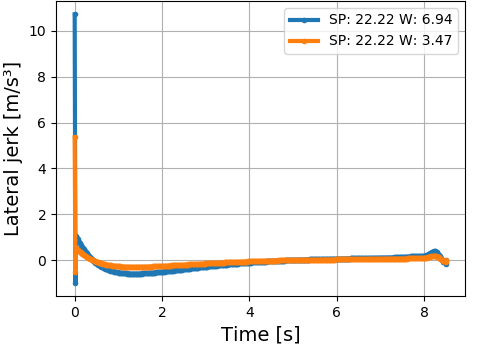
\includegraphics[width=1.0\linewidth]{jerk_num.png}
		%		\captionof{figure}{Lateral jerk using \ref{eq:diff}.}	
	\end{minipage}%
	\begin{minipage}{.5\textwidth}
		\centering
		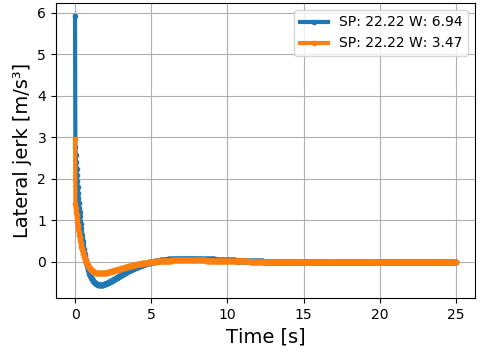
\includegraphics[width=1.0\linewidth]{jerk_ana.png}
		%		\captionof{figure}{Lateral jerk using appendix \ref{app:A} .}	
	\end{minipage}
	\caption{A comparison between the numerical jerk (left) based on Eq. (\ref{eq:diff}) and Eq. (\ref{eq:bicycle_model1}) and the analytical jerk (right) based on appendix \ref{app:A} and Eq. (\ref{eq:bicycle_model2}). }
	\label{fig:comp_jerks}
\end{figure}

It is clear that the analytical formulation (right figure)  of the jerk gives more smooth results and less high peaks which is in line with observations of the more complex $15$ dof Amesim vehicle that is discussed in chapter \ref{cha:Tracking_MPC}. Therefore the analytical formulation approaches reality better. An other way to see this is that the analytical formulation contains more information about the vehicle i.e. the equations resulting from numerical differentiation are approximations of the analytical ones.

\subsubsection{Initial guess}
To determine if the generated data is a local solution, two different initial guesses $V0:22.22 - L3.47$ and $V0:25.00 - L6.94$ are used whereof the retrieved data feature values are summarized in table \ref{tab:GD_local_test}. $V_0$ is the initial speed and L the lateral distance of the lane change used as initial guess and are generated using the above described numerical formulation. In order to calculate the data features displayed, time limit is set on $30\hspace{1mm}s$, N on $1000$, $V_{0} = 22.22\hspace{1mm}\frac{m}{s}$ and $L = 3.47\hspace{1mm}m$ as parameters in Eq. (\ref{opt:basic_opti_w}) and the analytical formulation is used. From the results it is suggested that the generated data feature values are not a local solution because they are found back from different start points of the optimization. During the learning of the weights as described in Figure \ref{fig:basic learning} the initial guess is set equal to the observed data. 

\begin{table}[h!]
	\centering
	\begin{tabular}{@{}llr@{}} \toprule
		\textbf{Feature Value}     & V0:22.22 - L3.47 & V0:25.00 - L6.94\\ \midrule
		Nr.1       & 6.83e-8   & 6.83e-8 \\
		Nr.2       & 0.37        & 0.37  \\
		Nr.3       & 1.77e-7     & 1.77e-7 \\
		Nr.4       & 0.57    & 0.57  \\
		Nr.5       & 1.98e-6     & 1.98e-6 \\
		Nr.6       & 30.94      & 30.94\\ \bottomrule
	\end{tabular}
	\caption{This table shows the retrieved feature values using the two different  initial guesses in Eq. (\ref{opt:basic_opti_w}).}
	\label{tab:GD_local_test}
\end{table}

\subsubsection{Time limit}
In order to check the dependency of the generated data on the chosen $T_{limit}$ constraint in Eq. (\ref{opt:basic_opti_w}), data is generated for a lane change with N, the amount of control points equal to $1000$, initial velocity equal to $80 \hspace{1 mm} \frac{km}{h}\hspace{1mm}(V_{0})$, a desired lateral displacement of $3.47\hspace{1mm}m\hspace{1mm}(L)$ and a varying $T_{limit}$ constraint as indicated in table \ref{tab:GD_time_limit}. Figures that  show what the difference in feature values actually means for the different kinematic signals of the vehicle, can be consulted in Appendix \ref{app:B}.

\begin{table}[h!]
	\centering
	\begin{tabular}{@{}llllr@{}} \toprule
		\textbf{Feature Value}    & 20 s  & 50 s      & 100 s\\ \midrule
		Nr.1       & 3.66e-8     & 1.13e-7   & 2.04e-7\\
		Nr.2       & 0.37        & 0.38      & 0.38\\
		Nr.3       & 1.13e-7     & 3.98e-7   & 1.56e-6 \\
		Nr.4       & 0.58        & 0.57      & 0.54\\
		Nr.5       & 1.72e-6     & 2.27e-6   & 3.16e-6\\
		Nr.6       & 31.05       & 30.74     & 30.42\\ \bottomrule
	\end{tabular}
	\caption{This table shows the retrieved feature values using different time limits in Eq. (\ref{opt:basic_opti_w}).}
	\label{tab:GD_time_limit}
\end{table}
Looking at even greater time limits is not desirable because beyond a time limit of $100 \hspace{1mm}s$, the time discretization gets larger than $0.1\hspace{1mm}s$ for N equal to $1000$ which will result in an unreliable discretization.\\

From the result of table \ref{tab:GD_time_limit} it can be concluded that the influence of the manually setting of the time limit in Eq. (\ref{opt:basic_opti_w}), can be neglected. 


\subsubsection{Amount of control points}
The test carried out to investigate the dependence of the resulting features values on the amount of control points $N$, uses the same parameters as described in the previous section but fixes the time limit on $30\hspace{1mm}s$ and varies N over $500$, $1000$ and $1500$ points. The results are shown in table \ref{tab:GD_N} whereof it follows that a choice of N equal to $1000$ is justified considering the small difference of the obtained features when N is equal to $1500$. For a full overview of the different kinematic signals, reference is made to Appendix \ref{app:B}.

\begin{table}[h!]
	\centering
	\begin{tabular}{@{}llllr@{}} \toprule
		\textbf{Feature Value}    & 500 s  & 1000 s      & 1500 s\\ \midrule
		Nr.1       & 9.42e-8     & 6.63e-8   & 6.45e-8\\
		Nr.2       & 0.38        & 0.37      & 0.37\\
		Nr.3       & 5.61e-7     & 1.77e-7   & 1.11e-7 \\
		Nr.4       & 0.56        & 0.57      & 0.58\\
		Nr.5       & 2.50e-6     & 1.98e-6   & 1.85e-6\\
		Nr.6       & 30.66       & 30.94     & 31.05\\ \bottomrule
	\end{tabular}
	\caption{This table shows the retrieved feature values using different amount of control point N in Eq. (\ref{opt:basic_opti_w}).}
	\label{tab:GD_N}
\end{table}


\subsubsection{Linear tire model}
In this section it is checked if the conditions to use a linearised lateral tire model is valid. In literature \cite{TongDuySon2019} it was found that this is the case when there are small lateral accelerations ($a_y <= 4 \frac{m}{s^2}$) and slip angles ($\alpha <= 5^o $) during the maneuver. Figure \ref{fig:lat} gives the total lateral acceleration during a lane change maneuver that moves around two lanes or an estimated lateral distance of $6.94 m$. Figure \ref{fig:slip} shows the slip angle during this maneuver. From the graphs it can be concluded that the linearisation of the lateral tire forces is valid and there is no need for a more complex tyre model embedded in Eq. (\ref{opt:basic_opti_w}).  Both resulting figures are generated with the complex vehicle model discussed in chapter \ref{cha:Tracking_MPC} and making use of Eq. \ref{eq:bicycle_slipangle} in order to estimate the slip angle.

 \begin{figure}[h!]
	\centering
	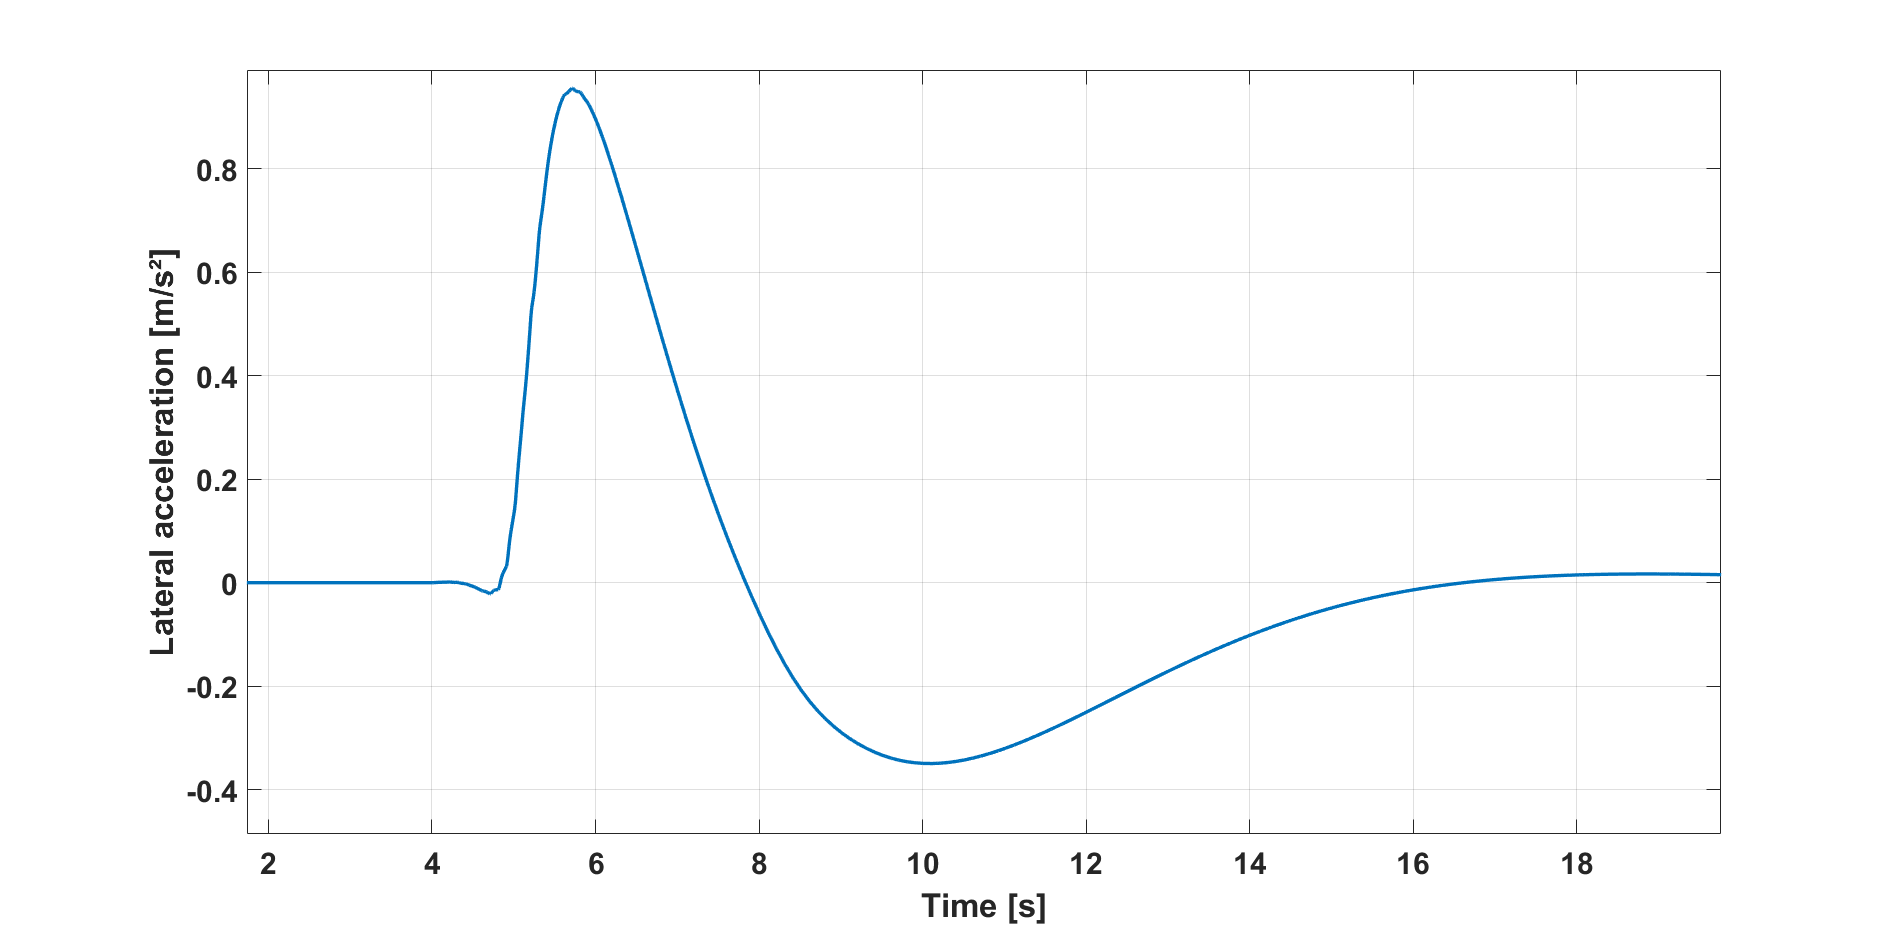
\includegraphics[width=1.0\textwidth]{lat_acc.png}
	\caption{Lateral acceleration during a lane change $V_0: 25.00 \frac{m}{s}$ and $L:6.94 m$ generated with the amesim model.}
	\label{fig:lat}
\end{figure}

 \begin{figure}[h!]
	\centering
	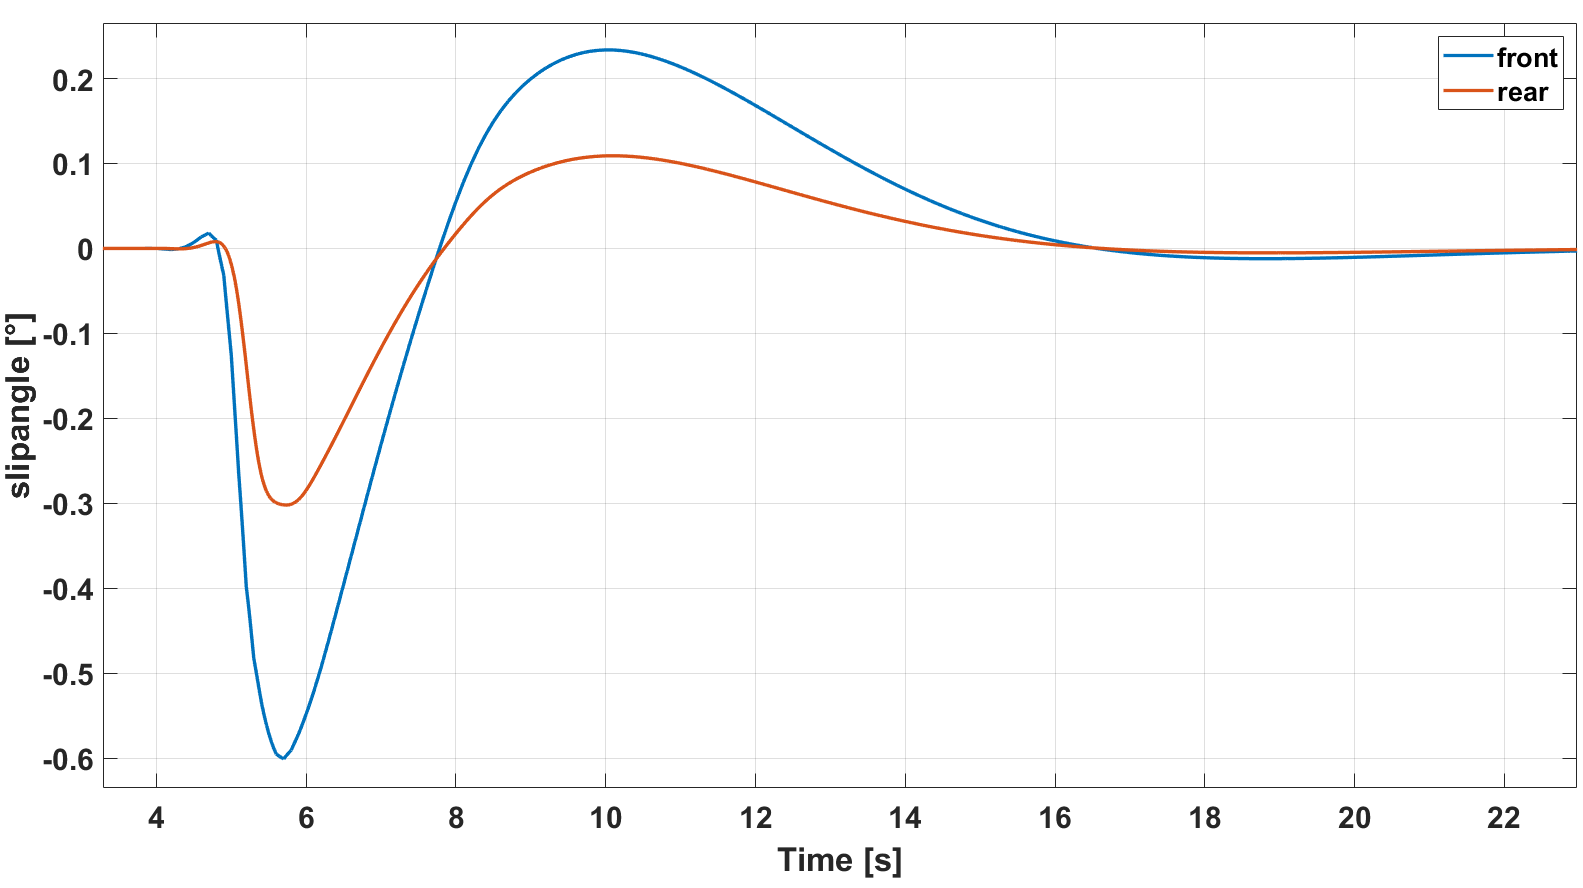
\includegraphics[width=1.0\textwidth]{slipangle_V25.00-L6.94-amesim.png}
	\caption{slip angle during lane change $V_0: 25.00 \frac{m}{s}$ and $L:6.94 m$ generated with the amesim model.(bleu:front,red:rear)}
	\label{fig:slip}
\end{figure}


\subsubsection{Feature values} \label{s:fv_val}
% Steeds dezelfde als enkel horizontale init speed verandert --> zelfde gewichten zullen geleerd worden aangezien enkel de lateral featues bijdragen. 
In the above tables it can be seen that the first, third and fifth feature values concerning longitudinal behaviour of the vehicle are very small. This often means that during a lane change these features have a low influence. It can be expected that for small observed feature values, it becomes hard to accurately learn weights that generate feature values that match with these small values. The reason for this is because the feature value is negligible which means that any weight times zero stays zero in the objective function of Eq. \ref{opt:basic_opti_w}. For this reason almost any weight can be used for the longitudinal features without observing a different lane change outputted by the optimization done in Eq. \ref{opt:basic_opti_w}. This will be further discussed in section\ref{s:SDL}.\\% A suggested solution for this is the use of different features or an different maneuver. Scaling in the calculation of the gradient doesn't help. RPROP update is independent of the order of size of the gradient. 

An other interesting thing to note about the generated data features is that when the initial speed of the lane change is varied and the desired lateral displacement stays the same ($3.47m$ or $6.97m$), because of the small longitudinal features values the data features found are almost identical. 

\subsubsection{Conclusion}
In this section there has been looked into the correctness of the generated data making use of Eq. (\ref{eq:bicycle_model2}), that further will be used to learn from. The influence of different choices i.e. the time limit and the amount of control points has been checked. Out of this it followed that it is allowed to take the time limit equal to $30 \hspace{1mm}s$ and the amount of control points to $1000$ as is done further on in this thesis. Next it has been shown that it is justified to use a linearised tire model. Finally the resulting feature values of the ideal data were shortly look into. It was concluded that a worse learning is expected for the retrieved longitudinal features due to their small values. 

\section{Ideal data learning results} \label{s:ID_results}
In this section the results of learning weights from ideal data is discussed.
Section \ref{s:SDL} concerns the learning of a single dataset $V_0:22.22\hspace{1mm}\frac{m}{s},\hspace{1mm} L:3.47\hspace{1mm}m$. In reality one demonstrated demonstration doesn't capture perfectly the preference of a human driver. In order to do so, learning of multiple datasets is needed. Therefore the averaging method is presented in section \ref{s:averaging_method} and the conflict method in section \ref{s:conflict_method}. Afterwards a comparison is made in section \ref{s:comparison of methods}.\\

It is known beforehand that the weights used to generate the data feature values are  $\bigl[ \begin{smallmatrix} 4,&5,&1,&6,&1,&2\end{smallmatrix}\bigr]$\footnote{The corresponding features  of the chosen weights can be seen in section \ref{s:obj} and are summarized by $\bigl[ \begin{smallmatrix} f_{ax},&f_{ay},&f_{jx},&f_{jy},&f_{diff vx},&f_{diff y}\end{smallmatrix}\bigr]$.} and the initial guess of the weights is chosen as an all one vector. The convergence criteria to stop the learning loop as displayed in Figure \ref{fig:basic learning}, is when the maximum amount of iterations set to $300$ is reached or if the data feature values are accurately regenerated with learned weights.\\
This is quantified by $f_{rel,i} = \frac{f_{learned,i}}{f_{obs,i}} \leq 10^{-3}$.  $\bm{f}_{obs}$ equals the generated data feature vector retrieved according to section \ref{s:GD} and is constant during learning. $\bm{f}_{learned}$ is the feature vector calculated from the learned path and changes during every learning loop according to Figure \ref{fig:basic learning}. Convergence is reached when the three lateral feature values $2$, $4$ and $6$, that dominantly define the lane change, are accurately fitted for a certain set of weights.\\
		
\subsection{Single dataset learning}\label{s:SDL}
The generated data features that are supposed to be matched in section \ref{s:SDL}, can be seen in table \ref{tab:GD_local_test}.
The resulting weight vector $\bm{\theta}$ and $\bm{f}_{rel}$ outputted at convergence on iteration $28$ is displayed in table \ref{tab:comp_it}. The weight concerning the lateral acceleration (Nr.$2$) is taken as reference in order to compare the learned weights with the chosen ones. The results show that the lateral weights are found accurately back. Table \ref{tab:comp_it} also shows the results when the algorithm is manually set to run for $121$ iterations.
A clear difference between the lateral features that have an increased matching of $f_{rel,i}$ with an accuracy of $10^{-6}$ is seen. The convergence of the longitudinal features $f_{rel,i}$ towards one, didn't increase much because they are constraint in the accuracy that they can be learned. 

\begin{table}[h!]
	\centering
	\begin{tabular}{@{}llllr@{}} \toprule
					      & $It.28-\bm{\theta}$ & $It.28-\bm{f_{rel}}$ & $It.121- \bm{\theta}$ & $It.121-\bm{f_{rel}}$\\ \midrule
		Nr.1       		  &14.469        & 0.9907 	    & 10.021 &	1.0004	\\
		Nr.2              &5.000       & 0.9995       & 5.000 &   1.0000   \\
		Nr.3              & 3.045       & 1.0037       & 2.179 &  0.9976    \\
		Nr.4              & 5.977       & 1.0006       & 5.998 & 1.0000     \\
		Nr.5              & 3.689       & 0.9941       & 2.538 &   0.9892   \\
		Nr.6              & 1.998       & 1.0001       & 2.002 &  1.0000    \\ \bottomrule
	\end{tabular}
	\caption{This table shows the weights learned from the dataset $V_0:22.22\frac{m}{s}-L:3.47m$ and the according $\bm{f}_{rel}$ at a different amount of iterations.}
	\label{tab:comp_it}
\end{table} 

 As already suggested in section \ref{s:fv_val} this is because of the small size of the feature values of the longitudinal direction. Not very accurate learned longitudinal feature values will have a negligible influence on the overall behaviour of the planned path and as can be seen, a range of weights will give an acceptable match quantified by $f_{rel,i}$.\\
 In order to learn the longitudinal weights of the human driver accurately, a maneuver should be considered were these features will be more prominent e.g. an acceleration maneuver or different features can be chosen e.g. $a_{tot}^2 = a_x^2 + a_y^2$. Because the interest in the longitudinal weights during a lane change is marginal this is not further discussed during this thesis.\\          

It could be argued that if the longitudinal feature weights are not so important in defining the lane change, they have to be removed from the objective Eq. (\ref{eq:obj}). This is however not an correct assumption. The longitudinal features are less determined during a lane change and therefore different weights give rise to the same lane changes. However, they still play a roll in comfortable path planning in order to avoid nervous throttle and consequently longitudinal jerk and acceleration behaviour. 


\subsection{Averaging method}\label{s:averaging_method}
In order to simultaneously learn from multiple datasets the averaging method is proposed. \cite{Kuderer2015a} The flow of the algorithm is similar as shown in Figure \ref{fig:basic learning} and the convergence criteria stays the same. However, instead of inputting a data feature vector $\bm{f}_{obs}$ based on a single dataset, an averaged one over multiple datasets is used.\\
To calculate the gradient used to update the weights $\bm{\theta}$, the difference between the averaged data feature vector and the averaged learned feature vector is taken. In order to obtain the averaged learned feature vector, $m$ times the optimization Eq. (\ref{opt:basic_opti_w}) is called with $m$ the amount of observed maneuvers. After solving the $m$ resulting learned feature vectors they are averaged. Each distinct maneuver has a different initial longitudinal speed and desired lateral displacement.\\
 
 % Bespreek de fixed feature approach.

The datasets chosen to perform the learning on are: $V_0:22.22\hspace{1mm}\frac{m}{s}-\hspace{1mm} L:3.47\hspace{1mm}m$, $V_0:25.00\hspace{1mm}\frac{m}{s}-\hspace{1mm} L:3.47\hspace{1mm}m$ and $V_0:22.22\hspace{1mm}\frac{m}{s}-\hspace{1mm} L:6.94\hspace{1mm}m$. The resulting weighs and average $\bm{f}_{rel}$ found after $25$ iterations are respectively $\bigl[ \begin{smallmatrix} 14.459,&5.000,&3.204,&5.984,&3.720,&2.000\end{smallmatrix}\bigr]$ and $\bigl[ \begin{smallmatrix} 0.9981,&0.9996,&0.9829,&1.0000,&0.9946,&1.0001\end{smallmatrix}\bigr]$. This means that the lateral chosen weights are accurately found back. The $\bm{f}_{rel}$ of the individual datasets can be seen in table \ref{tab:in_av}. It is shown that there is a good match between the learned feature vectors and the individual data feature vectors.
 
\begin{table}[h!]
	\centering
	\begin{tabular}{@{}llllr@{}} \toprule
		\textbf{Feature}    & V022.22 - L3.47 & V022.22 - L6.94 & V025.00 - L3.47\\ \midrule
		Nr.1       		  &1.0000        & 0.9973 	    & 1.0064 		\\
		Nr.2              & 1.0002       & 0.9992       & 1.0001       \\
		Nr.3              & 0.9860       & 0.9816       & 0.9983       \\
		Nr.4              & 1.0012       & 0.9995       & 1.0010       \\
		Nr.5              & 0.9972       & 0.9948       & 0.9902       \\
		Nr.6              & 0.9999       & 1.0002       & 0.9999       \\ \bottomrule
	\end{tabular}
	\caption{This table shows the $\bm{f}_{rel}$ for each individual dataset at convergence using the average method.}
	\label{tab:in_av}
\end{table} 
Figure \ref{fig:3D_learned_path} shows the three initial guesses of the paths that make use of an all one weight vector in red, purple and brown. The finally learned paths can be seen in pink, grey and yellow. These paths lay exactly on the observed ones. From this it is concluded that matching of feature values which are scalars, give a good representation for matching performance of the 2D kinematic vehicle signals. The rest of the kinematic signals originating from the non-linear bicycle model can be seen in Appendix \ref{app:C}. 

 \begin{figure}[h!]
	\centering
	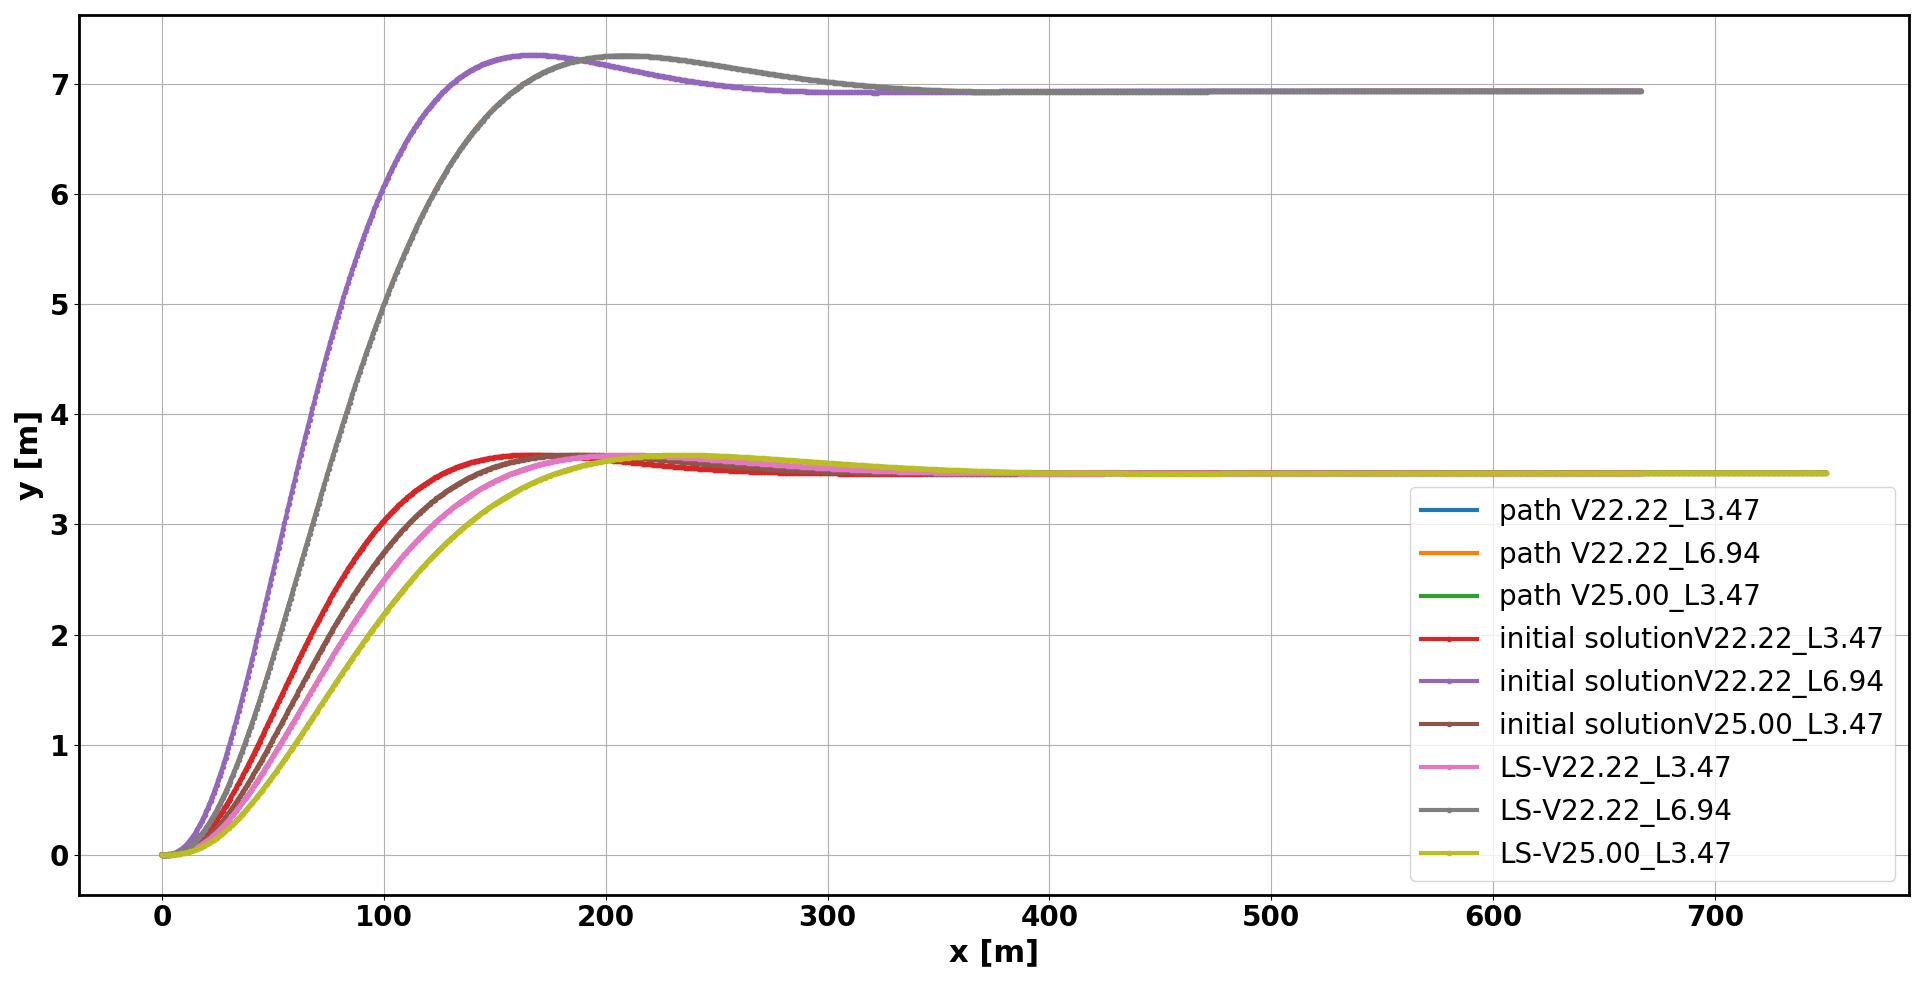
\includegraphics[width=1.0\textwidth]{3D_LP.png}
	\caption{Observed, initial and learned paths for 3 different observed lane changes generated with common underlying objective function.}
	\label{fig:3D_learned_path}
\end{figure}
 
The progress towards convergence over the iterations is showed in Figure \ref{fig:3D_conv}. Convergence is reached in $25$ iterations.

\begin{figure}[h!]
	\centering
	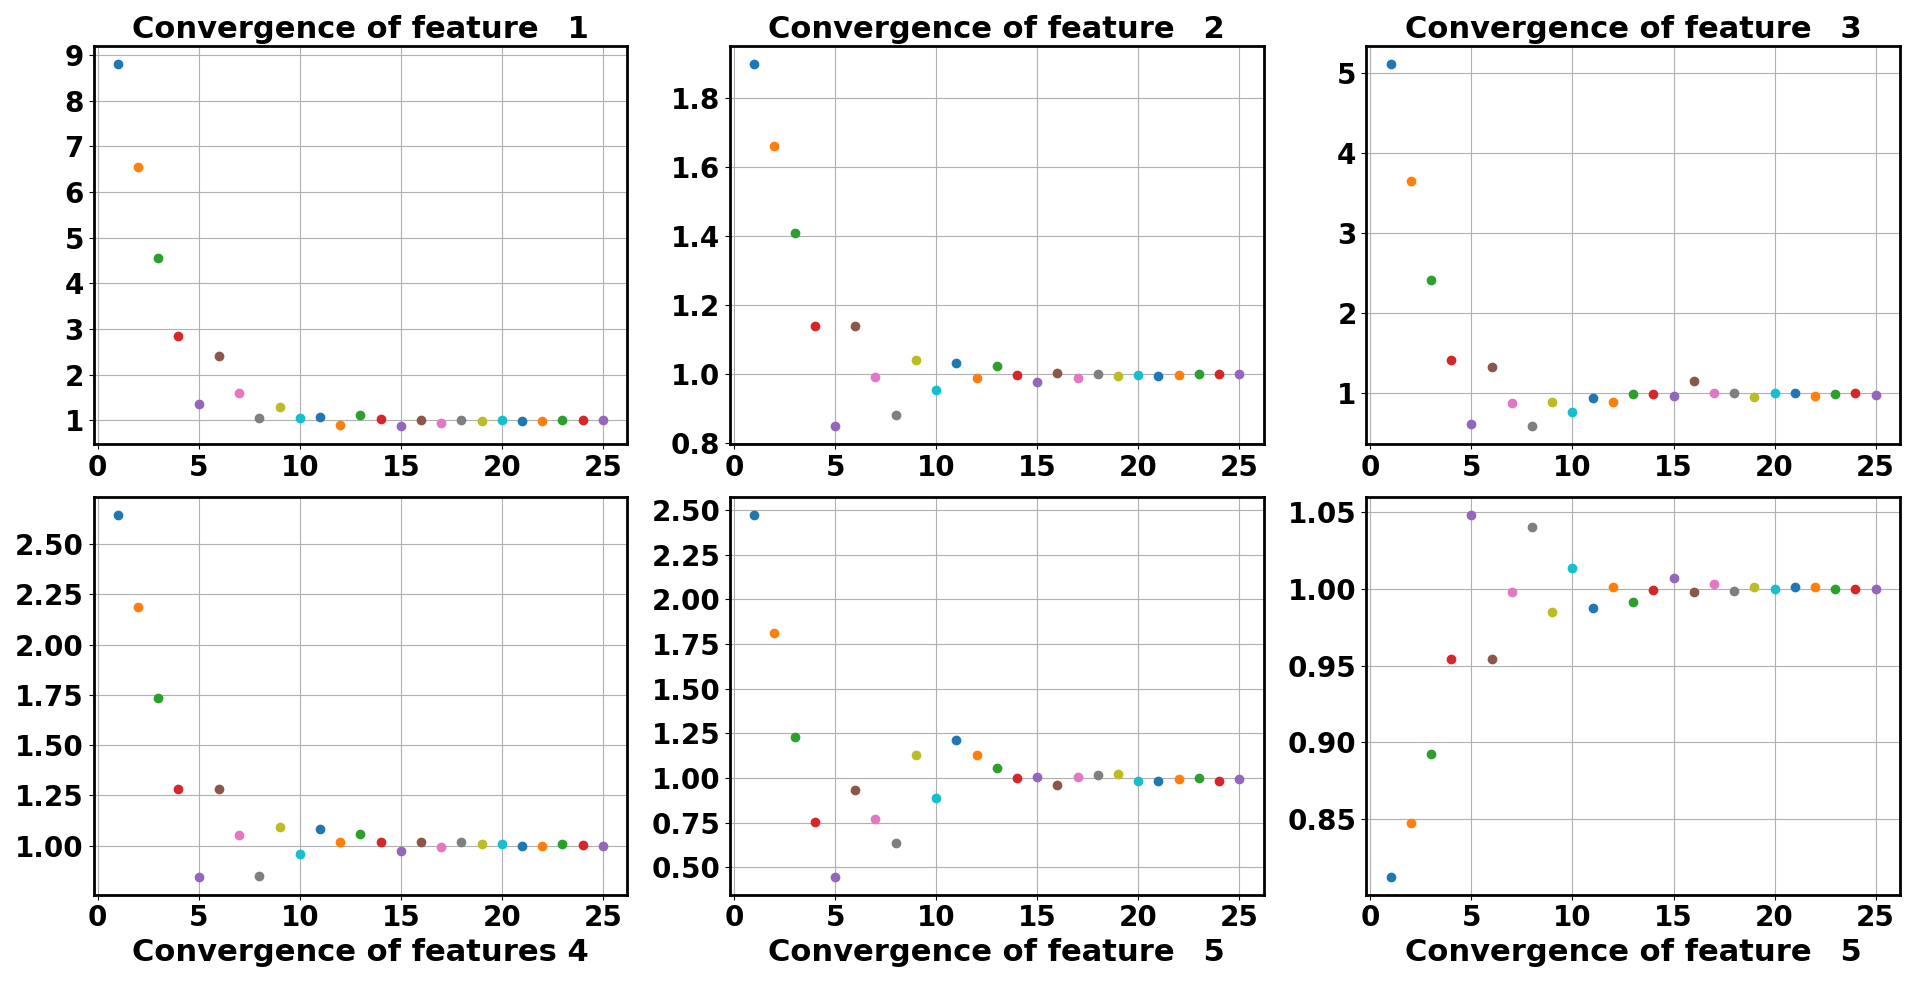
\includegraphics[width=1.0\textwidth]{3D_conv.png}
	\caption{The evolvement of the average $\bm{f}_{rel}$ over the learning iterations.}
	\label{fig:3D_conv}
\end{figure}

Figure \ref{fig:3D_w} gives a view of how the learned weights change over the iterations for the different features. The weights in these graphs differ with the ones shown at the beginning of this section by a scaling factor $\frac{5.0}{\theta_2}$. Both these weights will generate the exact same lane change when used in the objective of Eq. (\ref{opt:basic_opti_w}). During the learning process this degree of freedom can be removed by fixing the second weight equal to $5.000$. Convergence is reached after $59$ iterations and following weights are outputted $\bigl[ \begin{smallmatrix} 15.143,&5.000,&3.222,&6.016,&3.880,&2.007\end{smallmatrix}\bigr]$ where the lateral weights again clearly are found back. It takes the algorithm longer to find equivalent weights because of the lost in the ability of the RPROP algorithm to update all the weights. Therefore the scaling degree of freedom is retained during the rest of this thesis. \\

 
\begin{figure}[h!]
	\centering
	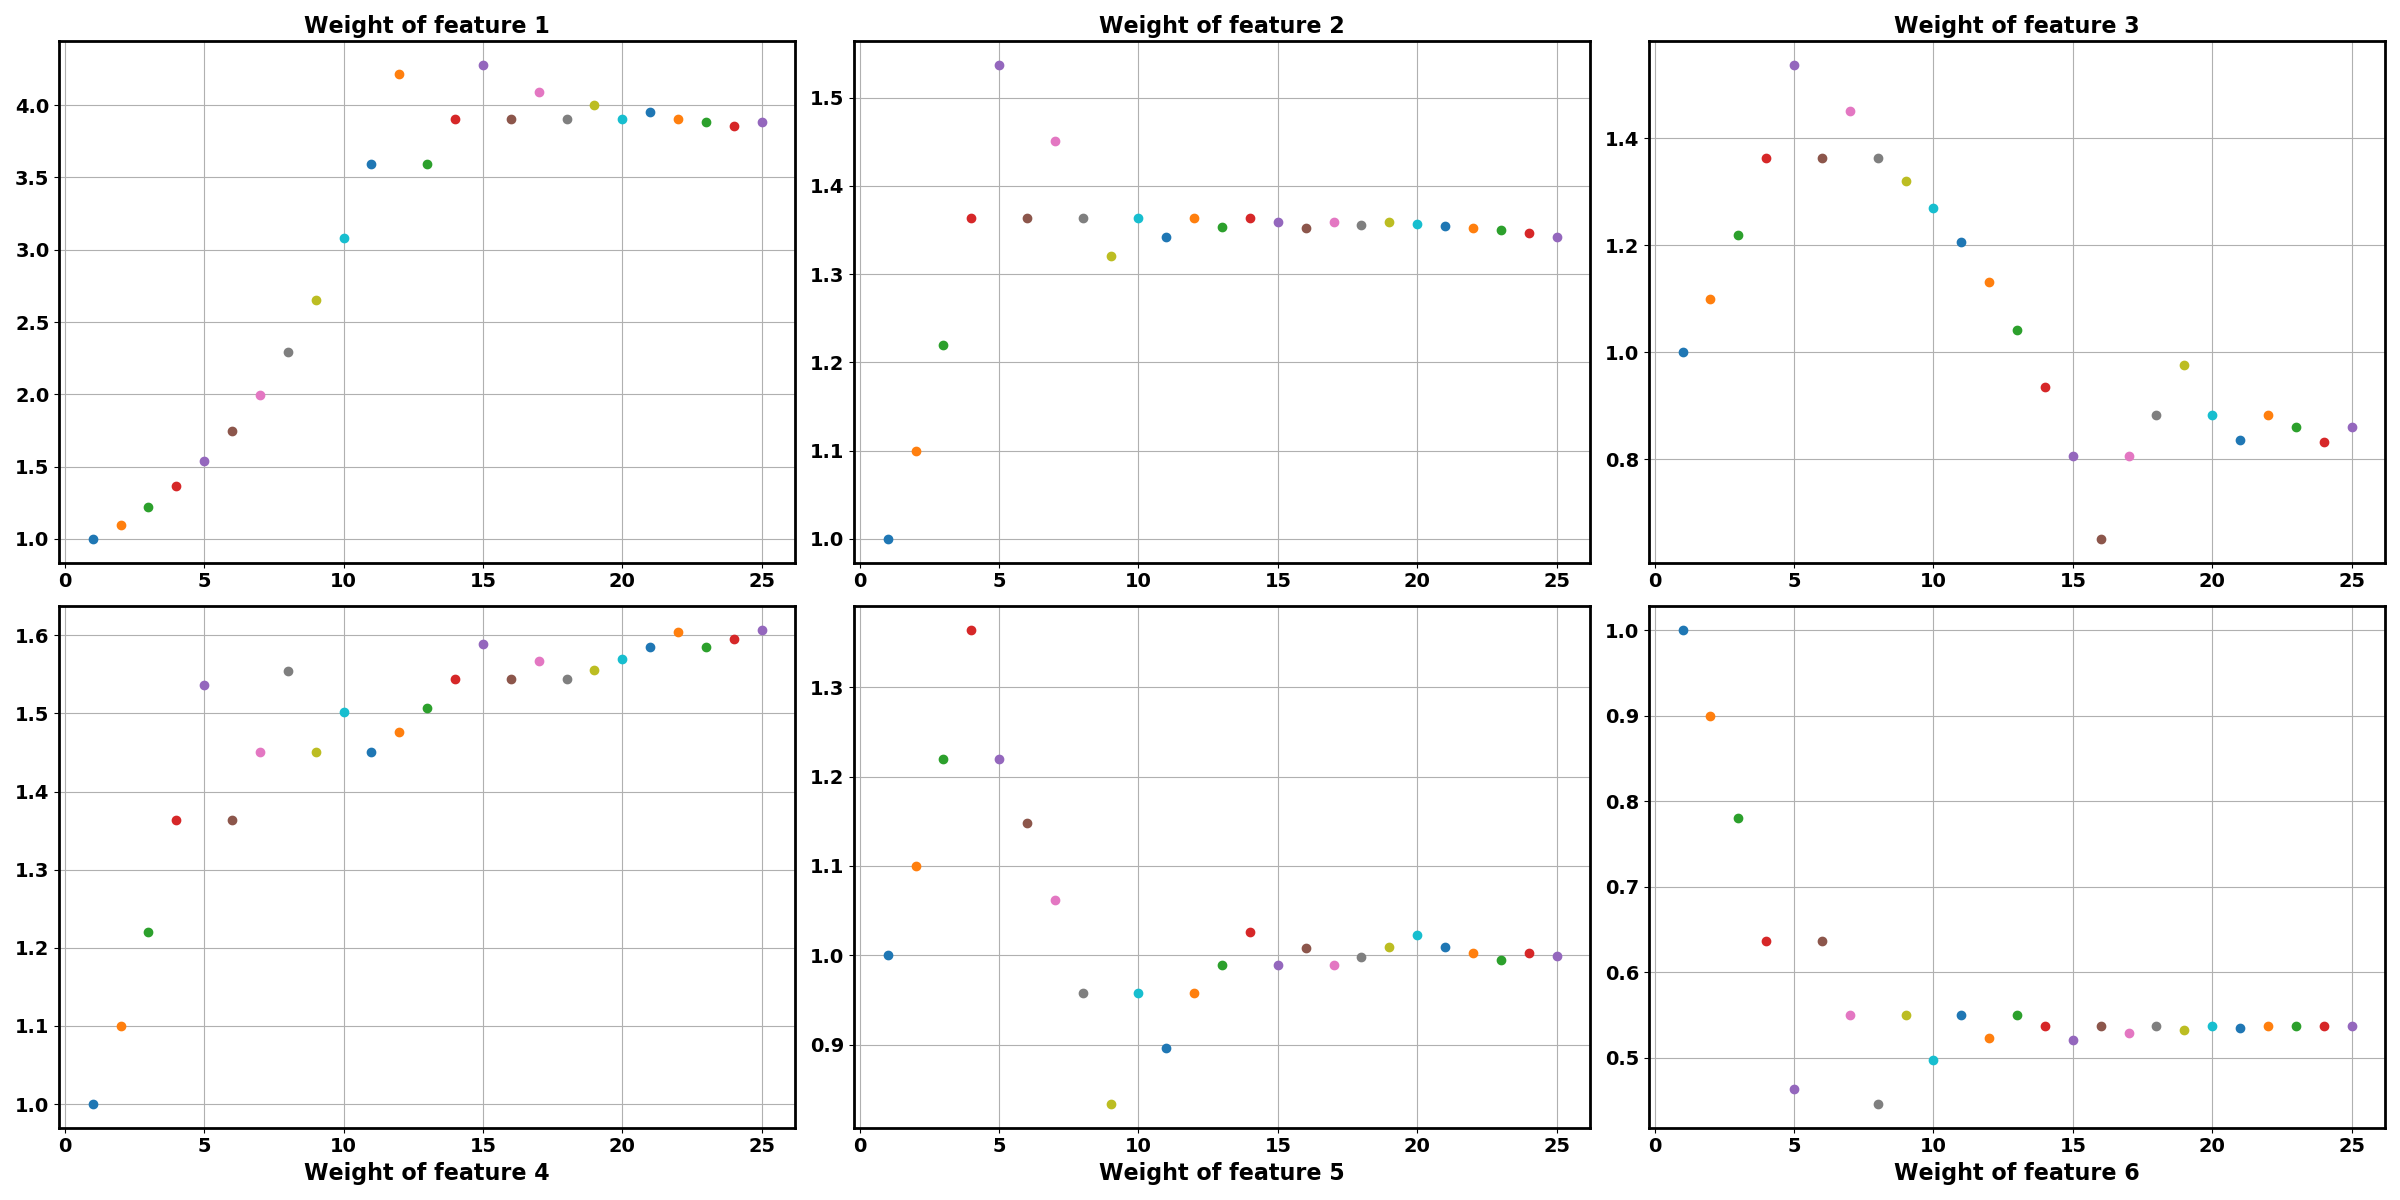
\includegraphics[width=1.0\textwidth]{3D_w.png}
	\caption{The different outputted weights over the learning iterations.}
	\label{fig:3D_w}
\end{figure}

\subsection{Conflict method}\label{s:conflict_method}
 The second method proposed to learn simultaneous of multiple datasets, is the conflict method. Its main idea is to only update a weight if the gradient, as given by Eq. (\ref{eq:new}), of the different individual datasets point all in the same direction. If there are individual gradients with conflicting signs, the update direction is ambiguous and the concerning weight is not updated. The updating will be resumed when the conflict is solved by updating the other weights. Solving conflicts is possible because the features are not independent of each other. Figure \ref{fig:conflict} shows how the conflict check is integrated together with the RPROP algorithm in the 'update weights' box in the basic learning flow of Figure \ref{fig:basic learning}. The blue boxes serve as output ports.\\
 
  \begin{figure}[h!]
 	\centering
 	\includegraphics[width=1.1\textwidth]{conflict.png}
 	\caption{Flow of the conflict method as part of the basic flow diagram of Figure \ref{fig:basic learning}}
 	\label{fig:conflict}
 \end{figure}

Depending if the previous case was RPROP case 2 and the sign difference between the current and previous gradient, three distinct RPROP cases can be identified which outputs the new update value, delta weights ($dw$) and the exception value as discussed in section \ref{s:RPROP}. Inside the conflict block, it is checked if all the signs of the current gradients are consistent. This boils down to verifying on which entry in the $m$ different gradients there is a sign difference. Here is $m$ the amount of observations and an individual gradient is calculated as  $\bm{F}_{obs,i} - \bm{F}(\bm{r}_{expected,i})$ with $m \in \mathbb{N}_{[1\dots ND]}$. \\ 

If there is a sign difference, this means that for one dataset the learned feature value is higher than the observed one and the corresponding weight should be increased (negative gradient) and for at least one other dataset, the corresponding weight should be decreased. (positive gradient) according to Eq. (\ref{eq:5}) and Eq. (\ref{eq:new}). For such a case the conflict test will give rise to a positive conflict value. If there is no conflict there will also be unity in the decision of the RPROP case, because no conflict was spotted in the gradients during the previous iteration. When a conflict is resolved, the next case will be automatically equal to case 3 because no decision can be made to either increase or decrease the update value. The convergence criteria used stays the same as discussed in \ref{s:averaging_method} but now an additional criteria is added that there should still be improvement possible. This means that it should be possible to update a weight in a direction that benefits every dataset.\\

The learning algorithm is applied on the same three datasets as discussed in section \ref{s:averaging_method} and uses as initial guess of the weights an all-one vector. The resulting weighs found after $32$ iterations are  $\bigl[ \begin{smallmatrix} 14.283,&5.000,&3.114,&5.979,&3.645,&2.000\end{smallmatrix}\bigr]$. The learning algorithm stopped because no update of the weights could be done without ambiguity. It can be concluded that the lateral weights are found back. The $\bm{f}_{rel}$ of the individual datasets can be seen in table \ref{tab:in_conflict}. The individual $\bm{f}_{rel,i}$ at convergence shows how good the match of feature values is when applying the learned weights at Eq. (\ref{opt:basic_opti_w}) with the same parameters for $V_0$ and $L$. It is shown in the table that there is a good match between the learned feature vectors and the individual data feature vectors. Figure \ref{fig:3D_conv_conflict} presents the convergence of the $\bm{f}_{rel}$ vector of dataset $V_0:22.22\frac{m}{s}- L:3.47m$. The individual convergence plots for the other datasets are very similar.

\begin{table}[h!]
	\centering
	\begin{tabular}{@{}llllr@{}} \toprule
		$\bm{f}_{rel}$    & V022.22 - L3.47 & V022.22 - L6.94 & V025.00 - L3.47\\ \midrule
		Nr.1       		  &0.9939       & 0.9913 	    & 1.0003 		\\
		Nr.2              & 1.0003       & 0.9993       & 1.0002       \\
		Nr.3              & 0.9911       & 0.9868       & 1.0032      \\
		Nr.4              & 1.0016       & 0.9999       & 1.0014       \\
		Nr.5              & 1.0009       & 0.9985       & 0.9941       \\
		Nr.6              & 0.9998       & 1.0001       & 0.9998       \\ \bottomrule
	\end{tabular}
	\caption{This table shows the $\bm{f_{rel}}$ for each individual dataset at convergence using the conflict method.}
	\label{tab:in_conflict}
\end{table} 


\begin{figure}[h!]
	\centering
	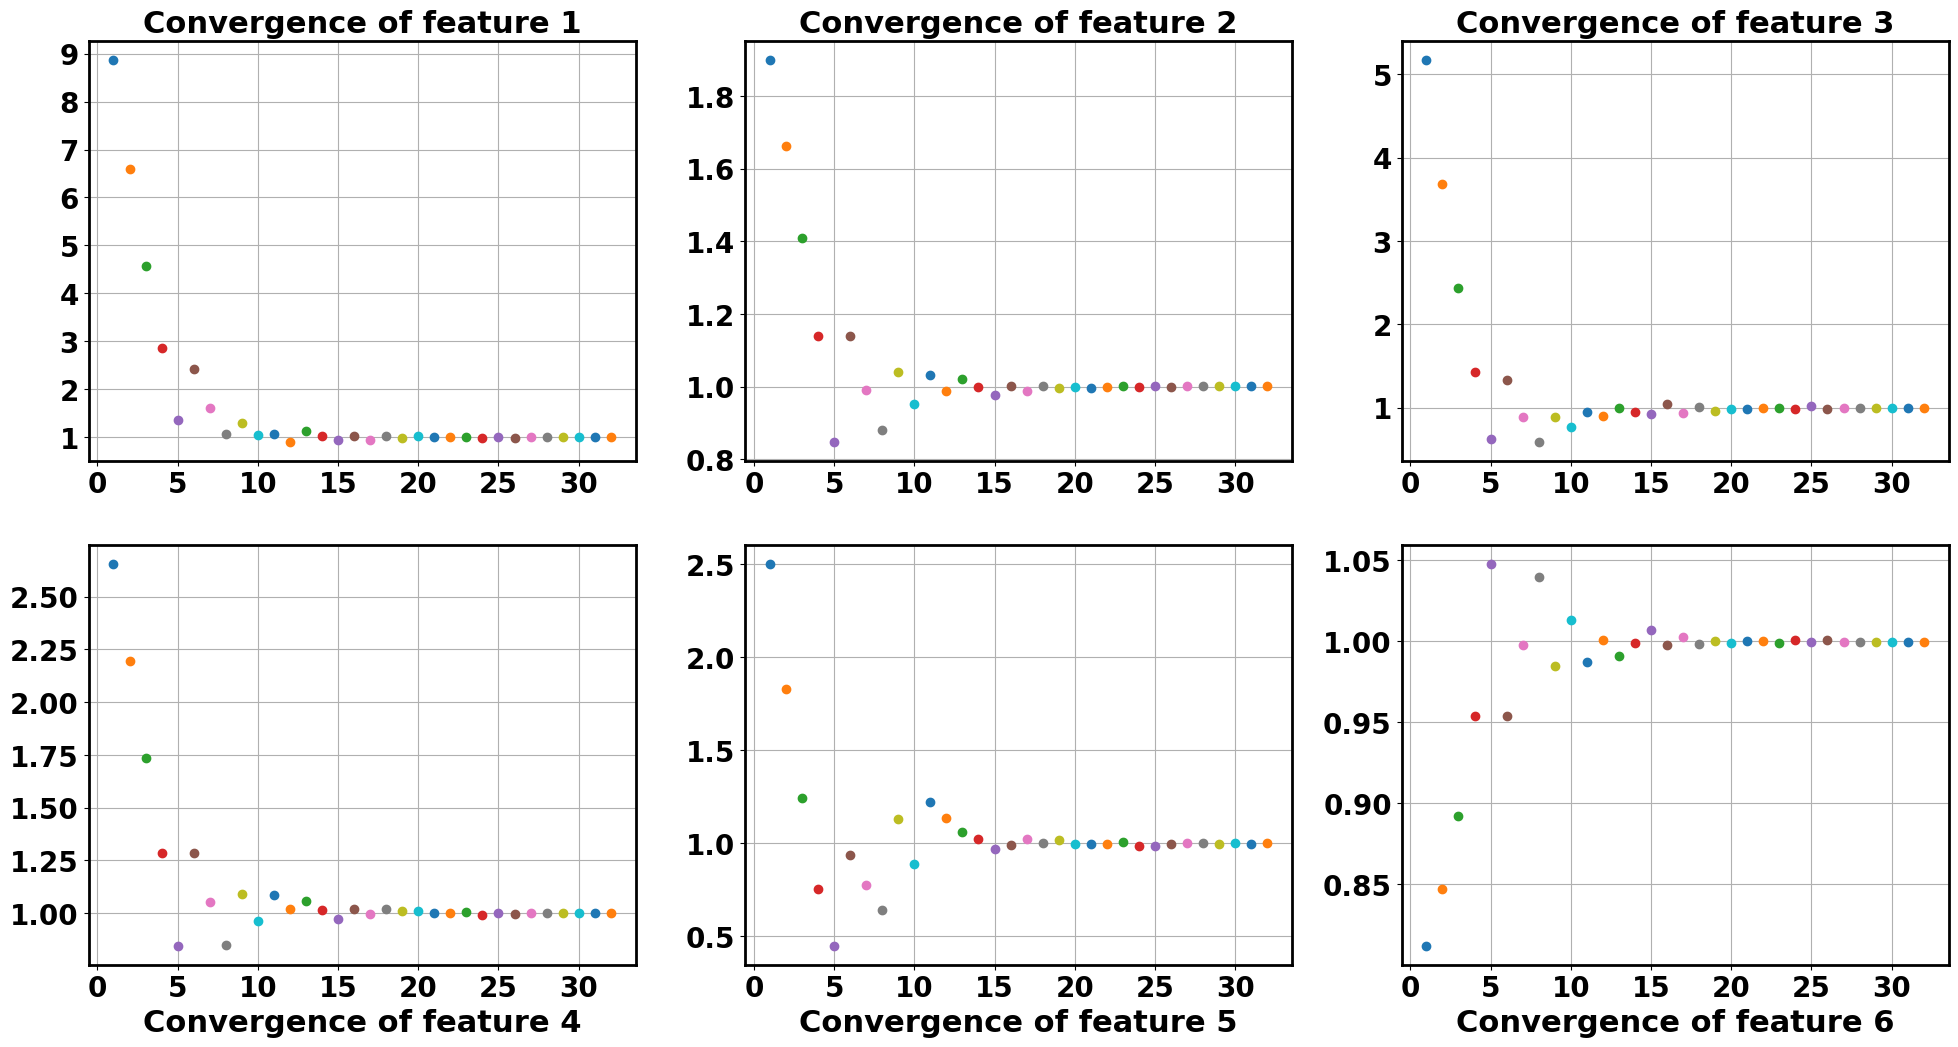
\includegraphics[width=1.0\textwidth]{3D_conv_conflict.png}
	\caption{The evolvement of $\bm{f}_{rel}$ of dataset  $V_0:22.22\hspace{1mm}\frac{m}{s},\hspace{1mm} L:3.47\hspace{1mm}m$ over the learning iterations.}
	\label{fig:3D_conv_conflict}
\end{figure}

As can be seen in table \ref{tab:in_conflict} and Figure \ref{fig:3D_conv_conflict} the conflict method is capable to give an adequate convergence towards the observed features. As is demonstrated in section \ref{s:averaging_method} when the feature values match, there is also a good match between the learned and demonstrated kinematic signals.\\
The algorithm was stopped because no improvement could be realized anymore. It could be hypothesized that if no ideal data is used where the human driver is less consistent in producing observations that resemble its underlying weights, the algorithm is stopped earlier. This will naturally constrict the algorithm in its feature matching accuracy due to no available direction of improvement. This can already be seen when more datasets are used in the conflict method e.g. 7 datasets. The algorithm stops then at $25$ iterations because it reached earlier a point of no improvement. The learned weights for 7 datasets are $\bigl[ \begin{smallmatrix} 14.785,&5.000,&3.223,&5.968,&3.770,&2.000\end{smallmatrix}\bigr]$. \\
Figure \ref{fig:acc_conflict} gives the averaged error that each individual $\bm{f}_{rel,i}$ vector makes with respect to convergence to one for the three important lateral features. The three important lateral features shown in Figure \ref{fig:acc_conflict} are respectively the remaining lateral distance, lateral acceleration and lateral jerk. $ND$ stands for number of datasets used.

\begin{figure}[h!]
	\centering
	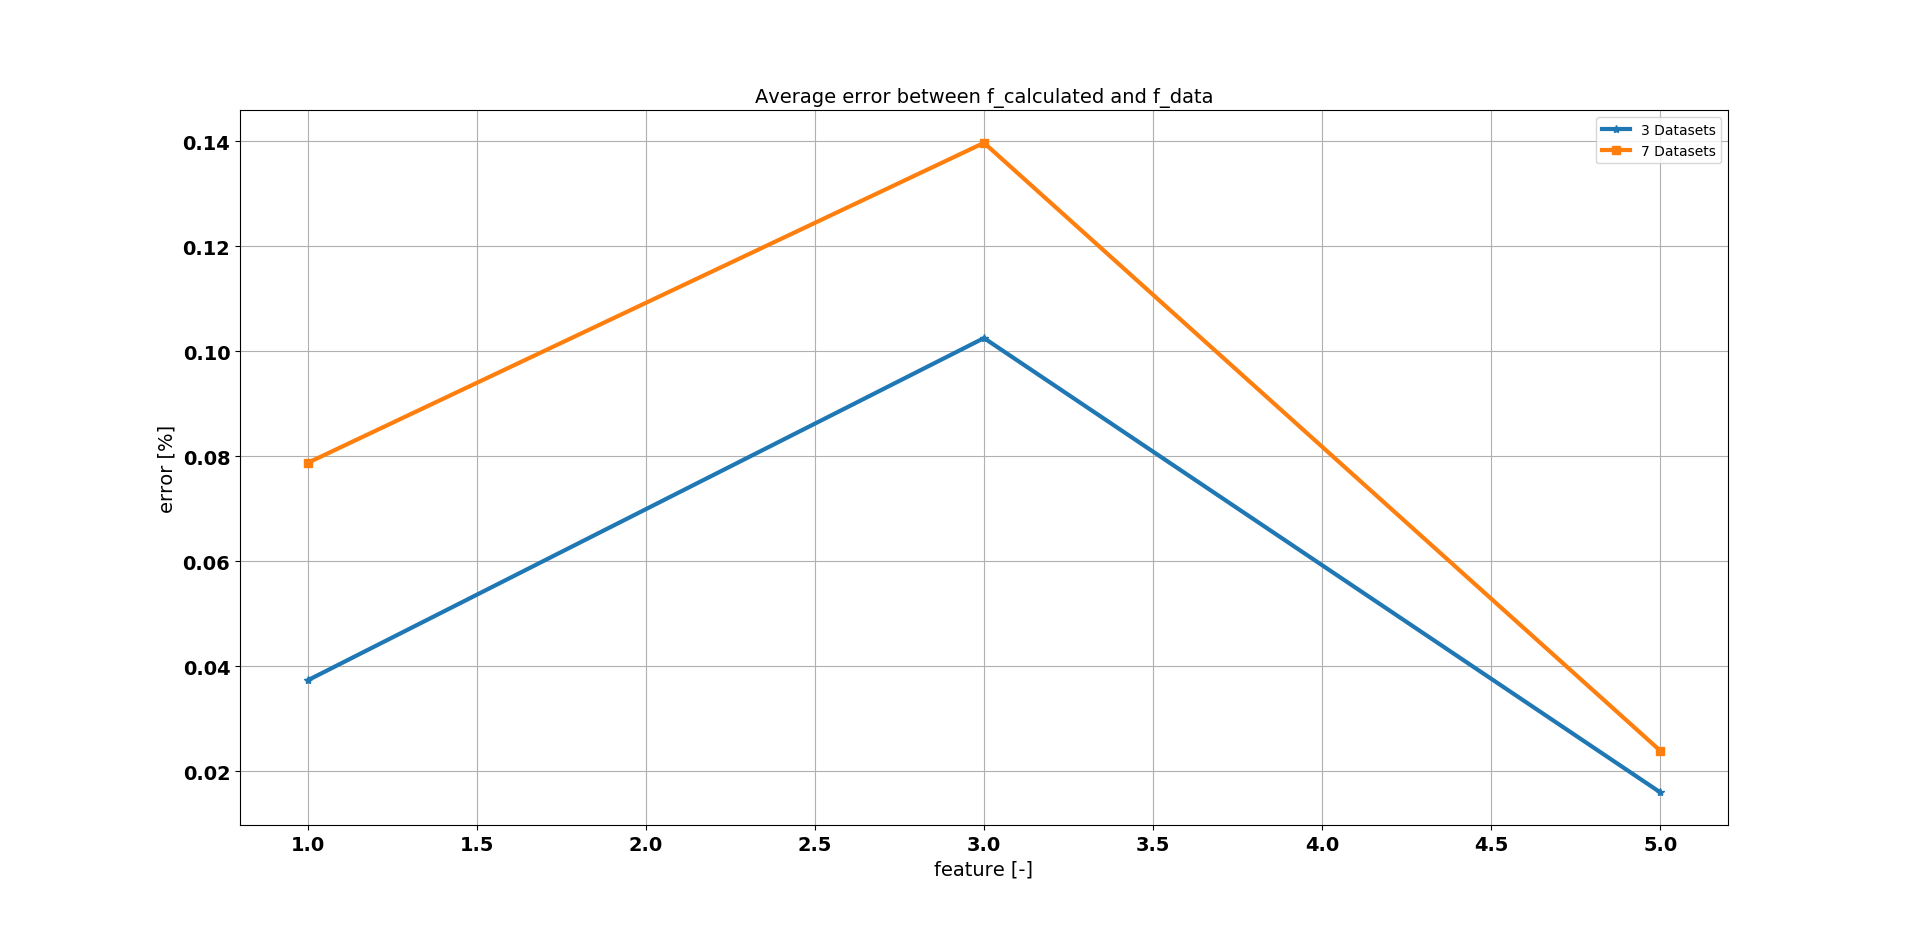
\includegraphics[width=1.1\textwidth]{acc_conflict.png}
	\caption{This figure shows the averaged, relative error given by $\frac{100\cdot\sum_{n=1}^{ND}|1-f_{rel,i}|}{ND}$ of the matching of the feature values for the three lateral features. (3 datasets: blue, 7 datasets: orange)}
	\label{fig:acc_conflict}
\end{figure}

Figure \ref{fig:acc_conflict} shows that the prematurely stop of learning with 7 datasets in comparison with 3 datasets gives an slightly higher error in the match of feature values of the individual datasets.    
 
\subsection{Comparison of methods}\label{s:comparison of methods}
In this section a comparison is made between the average and conflict method of combining multiple datasets. Figure \ref{fig:acc_comp} shows the averaged error defined as 

\begin{figure}[h!]
	\centering
	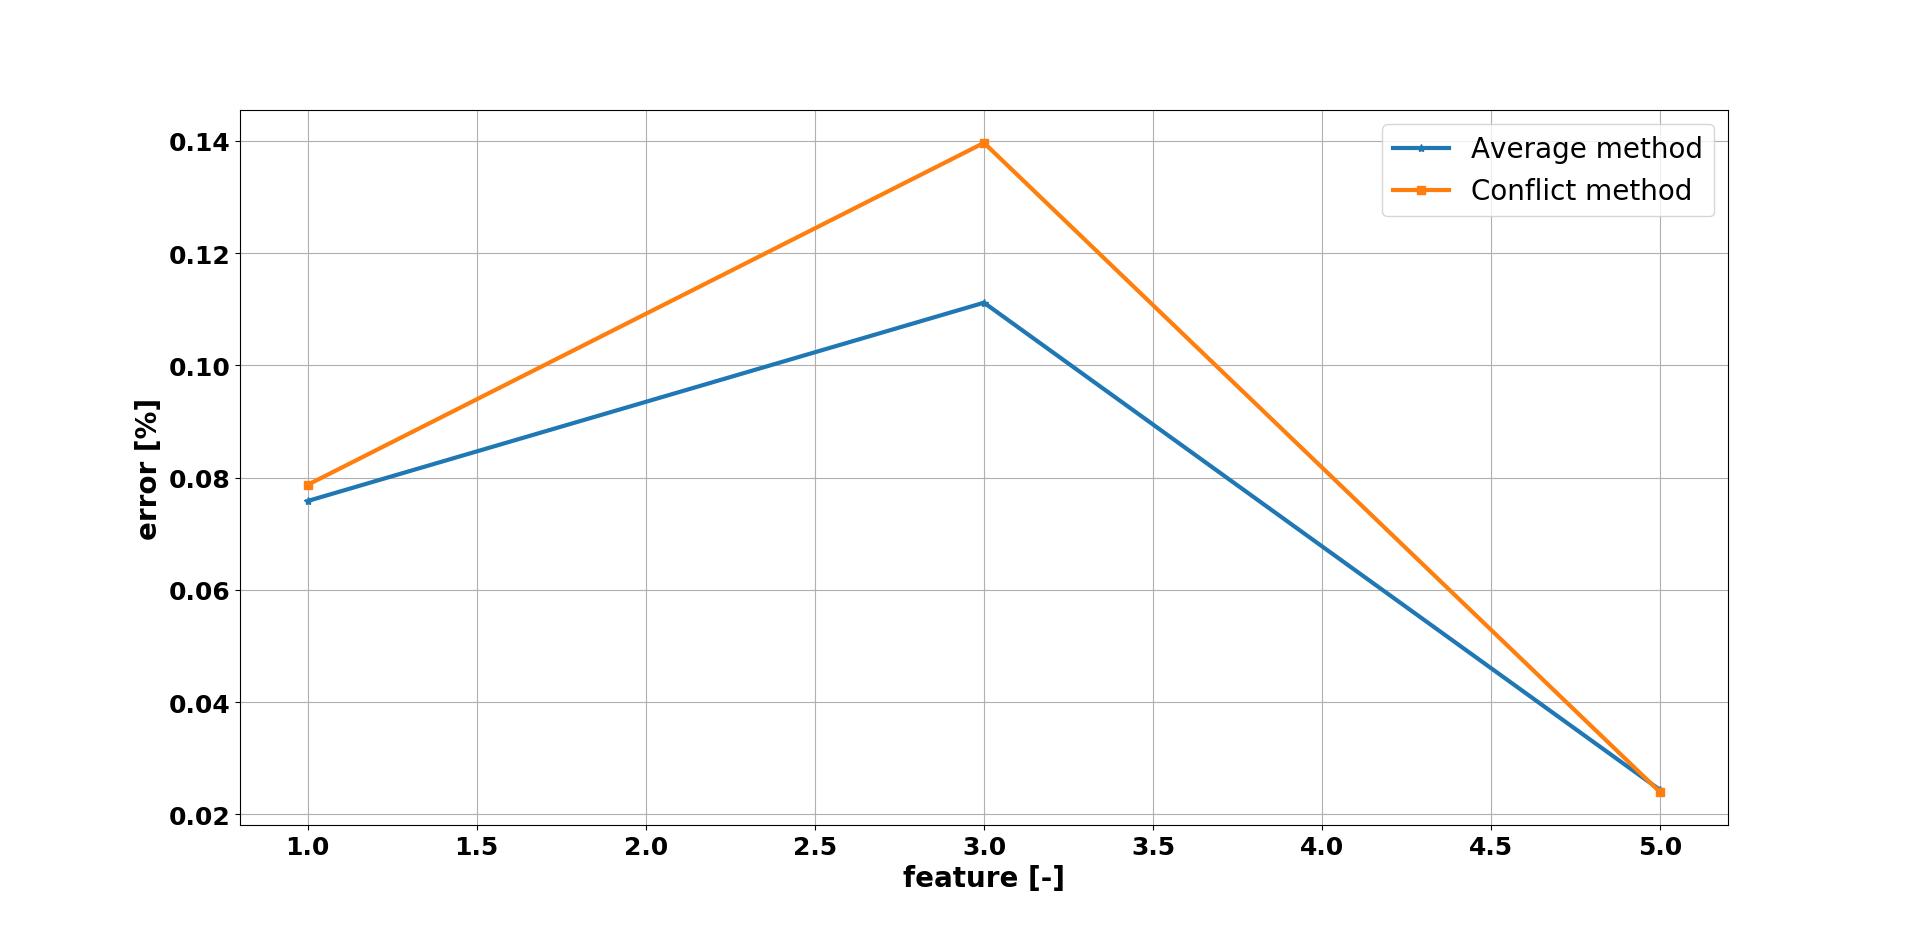
\includegraphics[width=1.0\textwidth]{acc_comp.png}
	\caption{This figure shows the averaged, relative error given by $\frac{100\cdot\sum_{n=1}^{ND}|1-f_{rel,i}|}{ND}$ of the matching of the feature values for the three lateral features. (Conflict method: blue, Averaging method: orange)}
	\label{fig:acc_comp}
\end{figure}

Because the averaging method gives slightly more accurate feature matching further in this thesis the averaging method is used.

 
 \section{Conclusion} \label{s:conclusion_cha4}
In this chapter the implementation of learning of ideal data was analysed. Data is considered ideal because it is produced with the same vehicle model as is used during the learning loop which calls the optimization Eq. (\ref{opt:basic_opti_w}). During this chapter first the non-linear bicycle model was discussed and its used parameters are presented in table \ref{table:vehicel_model_param}. Next a step by step building up of the learning algorithm is shown. It is displayed how the ideal data is generated and validated. Out of this it followed that the choice of number of control points was set on $1000$ and the time limit around $30 \hspace{1mm}s$. Afterwards the learning results were discussed and the conflict and averaging method were compared. It was concluded that for a lane change maneuver it is only important to learn the lateral weights accurately in order to explain the observed data. Feature matching was also accomplished for the longitudinal features but there was a boundary on the accuracy due to the small longitudinal feature values during a lane change. Because the conflict method gives for the same amount of datasets a slightly larger error on the ability to match feature values and because of the hypothesis that this method will behave worse when used with real driver data, the averaging method is chosen to be further used in this thesis. The estimate of the gradient $\pdv{\bm{F}_{diff}}{\bm{\theta}}$ by $\bm{F}_{obs} - \bm{F}(\bm{r}_{expected})$ was found adequate in order to match the learned and observed feature values.


%Dit is gemachtigd omdat men hier de omgeving wil scannen voor een feasible pad --> dit wordt trager gedaan dan de tracking.(tracking zal gebruik maken van een meer complex model) Path planning ligt focus vooral op de omgeving.
%Hoe zal de methode gevalideerd worden? Leg de twee methodes uit: code generatie en kijken of de wegings factoren terug gevonden kunnen worden? Mappen de feature values met de values van het geobserveerde pad? --> is het doel dat gevolgd probeert te worden haalbaar? 

%Vermeld afleiding van algortihm. Leg uit in Thesis hoe komt aan gradient die gebruikt. Zie papers: Ziebart et al and Kretzschmar et al.
%
%Modeleer een andere bestuurder. Can try to reproduce a data set with a change of parameters which represents a different driver. Can check that the learned model is also different. Hiermee aantonen dat er ook echt andere wegingsfactoren worden gegenereerd en dat de specifieke driving characteristics worden meegenomen.
%
%Ligt een tipje van de sluier op : hoe zal de data gegenereerd worden? 

%
%Maak een vermelding dat men het menselijke gedrag van het geleerde model kan nagaan met een Turing test.\\
%
%Maak een plotje zoals paper Learning to Predict Trajectories of Cooperatively Navigating Agents --> feature variance afwijking en average error. (zelfde plotjes als al de papers)\\
%
%Schrijf een paragraaf over hoe de data gegenereerd wordt. %
%
%Kan vermelding maken dat in deze thesis de features zijn gekozen met de hand --> men kan proberen om de features ook te leren van date (Characterizing Driving Styles with Deep Learning)
% Try to validate the chosen features with looking at the sensitivity.

%%Afleiding van exponentiël functie zie paper: Feature-based prediction of trajectories for socially compliant navigation (foto) --> weights are lagrange coefficients.


%\section{Tables}
%Tables are used to present data neatly arranged. A table is normally
%not a spreadsheet! Compare \tref{tab:wrong} en \tref{tab:ok}: which table do
%you prefer?
%
%\begin{table}
%  \centering
%  \begin{tabular}{||l|lr||} \hline
%    gnats     & gram      & \$13.65 \\ \cline{2-3}
%              & each      & .01 \\ \hline
%    gnu       & stuffed   & 92.50 \\ \cline{1-1} \cline{3-3}
%    emu       &           & 33.33 \\ \hline
%    armadillo & frozen    & 8.99 \\ \hline
%  \end{tabular}
%  \caption{A table with the wrong layout.}
%  \label{tab:wrong}
%\end{table}
%
%\begin{table}
%  \centering
%  \begin{tabular}{@{}llr@{}} \toprule
%    \multicolumn{2}{c}{Item} \\ \cmidrule(r){1-2}
%    Animal    & Description & Price (\$)\\ \midrule
%    Gnat      & per gram    & 13.65 \\
%              & each        & 0.01 \\
%    Gnu       & stuffed     & 92.50 \\
%    Emu       & stuffed     & 33.33 \\
%    Armadillo & frozen      & 8.99 \\ \bottomrule
%  \end{tabular}
%  \caption{A table with the correct layout.}
%  \label{tab:ok}
%\end{table}


%%% Local Variables: 
%%% mode: latex
%%% TeX-master: "thesis"
%%% End: 

\chapter{Learning from complex vehicle model}
\label{cha:Tracking_MPC}

%Plot simulink model en duidt de blokken aan die zullen worden ingevuld. Hier gaat dieper in gegaan worden in de volgende hoofdstukken. 

Because the non-linear bicycle model makes abstraction of dynamics that are applicable in a real vehicle, a more complex model is introduced to improve the reality factor of the simulations. In order to achieve this the $15$ degrees of freedom amesim model as can be seen in Figure \ref{fig:Amesim}, is provided by Siemens. The parameters of this model are tuned by the company in order to behave similar to a testcar they are currently using. The model has as inputs the amount of throttle, braking and steerwheelangle.  

\begin{figure}[h!]
	\centering
	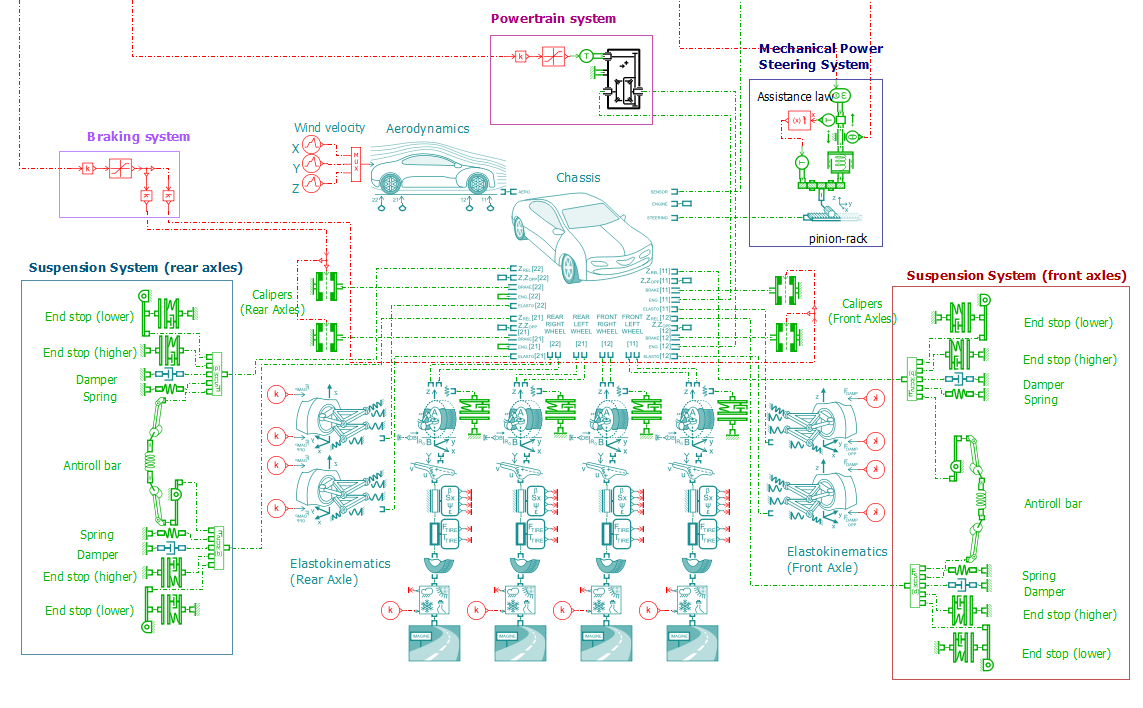
\includegraphics[width=1.0\textwidth]{Amesim.PNG}
	\caption{The 15 dof amesim model with as inputs the amount of throttle, braking and steerwheelangle.}	
	\label{fig:Amesim}
\end{figure}

The Amesim model serves as a black box and no direct dynamic equations are available 
to include in Eq. (\ref{opt:basic_opti_w}) as was done with the non-linear bicycle model Eq. (\ref{eq:bicycle_model_eqmotion}). Therefore a path is planned with the simpler non-linear bicycle model and afterwards a model predictive control tracking algorithm is applied on the Amesim model in order to follow its reference. The working principles of a MPC is discussed in \ref{s:MPC_e}. Diagram \ref{fig:complex_learning} shows the flow of handlings that is done during learning with the Amesim model.

\begin{figure}[h!]
	\centering
	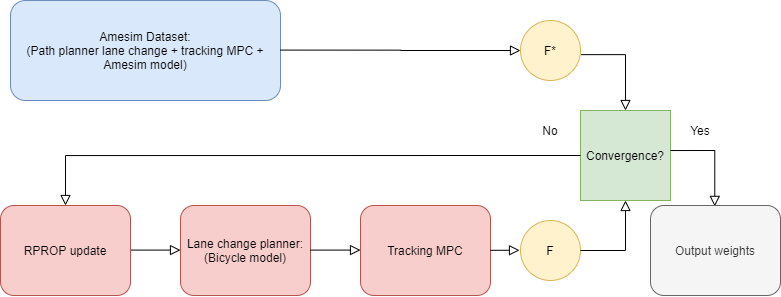
\includegraphics[width=1.1\textwidth]{complex_learning_diagram.PNG}
	\caption{The flow of learning with the Amesim model.}	
	\label{fig:complex_learning} 
\end{figure}

As is described in Diagram \ref{fig:complex_learning} the feature vector $\bm{F}(\bm{r})$ is calculated based on the path tracked by the Amesim model and used in the convergence block to estimate the gradient $\pdv{\bm{F}}{\bm{\theta}}$. The estimation is calculated by $\bm{F}_{obs} - \bm{F}(\bm{r}_{expected})$. The reason why the planned path has to be tracked is to avoid to include a vehicle mismatch error in the learning process. This that it is otherwise possible that even when the learning algorithm is capable to match the feature vectors $\bm{F}(\bm{r})$ and  $\bm{F}^*(\bm{r})$, coming form two different vehicle models, the learned kinematic signals of the bicycle model will not represent the observations produced by the Amesim model accurate enough. In order to check this, table \ref{tab:comparinson_models} \footnote{Note that the feature values of the bicycle model are slightly different than the ones in table \ref{tab:GD_local_test}. This is because in the previous table the time limit was set on $30 \hspace{1mm}s$ and here time limit is $25 \hspace{1mm}s$. This is done to have a better useable time discretization of $0.025\hspace{1mm}s$ to input as reference signal to the Amesim model.} shows the different feature values for a lane change $V_0:22.22\hspace{1mm}\frac{m}{s},\hspace{1mm} L:3.47\hspace{1mm}m$ generated with both the models.\\


\begin{table}[h!]
	\centering
	\begin{tabular}{@{}llr@{}} \toprule
		Feature Value    & Bicycle model & Amesim model\\ \midrule
		Nr.1       		 & 5.28e-8    & 3.33e-7 \\
		Nr.2       		 & 0.37       & 0.38  \\
		Nr.3       		 & 1.41e-7    & 1.20e-4 \\
		Nr.4       		 & 0.57       & 0.49  \\
		Nr.5       		 & 1.89e-6    & 9.40e-6 \\
		Nr.6       		 & 30.99      & 31.05\\ \bottomrule
	\end{tabular}
	\caption{This table shows the feature values of a lane change $V_0:22.22\hspace{1mm}\frac{m}{s},\hspace{1mm} L:3.47\hspace{1mm}m$ for respectively the Bicycle and Amesim model.}
	\label{tab:comparinson_models}
\end{table}

Out of table \ref{tab:comparinson_models} it can be concluded that the feature values, that will serve as the feature values of the observations and were produced using the bicycle and Amesim model, are almost the equivalent. However although the feature values of the observations were the same, not all kinematic signals also give an accurate match as can be seen in Appendix \ref{app:D}. This will further be discussed in section \ref{s:tracking_mpc}. 

This chapter also gives an answer in section \ref{s:complex_learning_results} on the question if the estimate of the gradient $\pdv{\bm{F}}{\bm{\theta}}$ by $ \bm{F}_{obs} - \bm{F}(\bm{r}_{expected})$ is still sufficient in order to match the learned and observed feature values.

\section{Tracking MPC} 
\label{s:tracking_mpc}
To be able to integrate the Amesim model in the learning process in an adequate manner, good tracking is desirable for the important lateral features that determine the lane change. A good tracking is therefore wanted for: $y(t), a_y(t)$ and $j_y(t)$.

\subsection{MPC formulation}
First the OCP that will be called during the MPC has to be defined. This is done by using the non-linear bicycle model defined with 10 states as seen in Eq. (\ref{eq:bicycle_model2}), inside the OCP formulation given by Eq. (\ref{opt:tracking}). Eq. (\ref{opt:tracking}) uses as objective an error function with respect to the reference with will assure the following behaviour. The control horizon of the MPC is $N_{MPC}$ and equal to $50$ points which means a control horizon of $1.25 \hspace{1mm}s$ because the reference is sampled with $T_{pl}$ equal to $0.025\hspace{1mm}s$. The parameters of the bicycle model stay the same as the ones listed in \ref{table:vehicel_model_param}. In order to formulate the gap closing constraint, which connects the previous states to the next in the chosen multiple shooting formulation, Runge-Kutta integration is embedded in function $I$.  
The first time that the OCP is solved and the current state is not yet outputted by the virtual sensors of the Amesim model, the initial states are set equal to the first reference point. The path constraints can be seen in Eq. (\ref{eq:F_MPC}). The path constraints are at first sight not necessary but contribute by decreasing the feasible solution space for the solver. It is checked that these constraints are not binding, which means that the found solution is reachable even if the constraints were removed. 

\begin{equation}\label{opt:tracking}
\begin{aligned}
\min_{\bm{X}(.),\bm{U}(.)} \quad &  E(\bm{X}(.),\bm{U}(.)) \\
\textrm{s.t.} \quad & \bm{X}^{k+1} = I(\bm{X}^{k}, \bm{U}^{k}) & k = [0,\cdots, N_{MPC}-1]\\
& \bm{X}^{0} = \bm{X}_{current} \\
& \bm{F}(\bm{X}^{k}) \geq 0	& k = [0,\cdots, N_{MPC}]\\
& \bm{X}^{k}\in \mathbb{R}^{10\times 1}  & k = [0,\cdots, N_{MPC}]\\
& \bm{U}^{k}\in \mathbb{R}^{2\times 1} \hspace{3 mm} & k = [0,\cdots, N_{MPC}-1]\\
&  N_{MPC} \in \mathbb{N}
\end{aligned}
\end{equation}

\begin{equation}\label{eq:F_MPC}
\bm{F} =
\begin{Bmatrix}
-\frac{Width\hspace{1mm}Lane}{2} \leq y^k \leq \frac{3\cdot Width\hspace{1mm}Lane}{2}, & k = [0,\cdots, N_{MPC}] \\
0 \leq x^k, & k = [0,\cdots, N_{MPC}] \\
-\frac{\pi\cdot 5}{180} \leq \psi^k \leq \frac{\pi\cdot 5}{180}, & k = [0,\cdots, N_{MPC}] \\
v_{x,start}-1 \leq v_x^k \leq v_{x,start}+1, & k = [0,\cdots, N_{MPC}]
\end{Bmatrix}
\end{equation}\

The error function that serves as the objective of the OCP is given by the following equation. The weights that gave the best tracking results are shown in table \ref{tab:weights}.

\begin{multline*} 
objective=W_1(\bm{x}[2:end]-\bm{ref}_x)^T(\bm{x}[2:end]-\bm{ref}_x)+W_2(\bm{y}[2:end]-\bm{ref}_y)^T(\bm{y}[2:end]-\bm{ref}_y)\\
+W_3(\bm{v}_x[2:end]-\bm{ref}_{v_x})^T(\bm{v}_x[2:end]-\bm{ref}_{v_x})+W_4(\bm{v}_y[2:end]-\bm{ref}_{v_y})^T(\bm{v}_y[2:end]-\bm{ref}_{v_y})\\+W_5(\bm{\psi}[2:end]-\bm{ref}_{\psi})^T(\bm{\psi}[2:end]-\bm{ref}_\psi)
+W_6(\bm{\dot{\psi}}[2:end]-\bm{ref}_{\dot{\psi}})^T(\bm{\dot{\psi}}[2:end]-\bm{ref}_{\dot{\psi}})\\ + W_7\dot{\bm{t}}_r^T\dot{\bm{t}}_r+W_8\dot{\bm{\delta}}_s^T\dot{\bm{\delta}}_s + W_9\dot{\bm{a}}_x^T\dot{\bm{a}}_x
\end{multline*}

\[\bm{x},\bm{y},\bm{v}_x,\bm{v}_y,\bm{\psi},\dot{\bm{\psi}},\bm{a}_x \in \mathbb{R}^{(N_{MPC}+1)\times1} \hspace{10mm}\bm{ref}_{i},\dot{\bm{t}}_r,\dot{\bm{\delta}}_s \in \mathbb{R}^{N_{MPC}\times1}\]


\begin{table}[h!]
	\centering
	\begin{tabular}{@{}lr@{}} 
		Weight    & Value\\ \midrule
		W1      & 10\\
		W2          & 10\\
		W3 	   & 30\\
		W4       & 1.0\\
		W5       & 100\\
		W6       & 1.0\\
		W7       & 5.0\\
		W8       & 0.01\\
		W9  & 0.01\\ \bottomrule
	\end{tabular}
	\caption{Overview of the weights used in the objective of Eq. (\ref{opt:tracking}).}
	\label{tab:weights}
\end{table}

The ultimate weights displayed were attained by trail and error but there is an intuitive explanation on why these states were used and which order of magnitude the weights were given.\\
It was first tried to focus on path tracking in order to see how the other states would differ when the Amesim model drove exactly the same path as the non-linear vehicle and therefore $x(t),y(t)$ and $\psi(t)$ were included. They define the orientation of the vehicle. Nervous input behaviour was noticed and in order to smooth the input, they were given a small weight. Only a small weight is given to assure  good tracking behaviour. It was observed that this strategy resulted in a good tracking of the important signals for the learning algorithm: $y(t), a_y(t)$ and $j_y(t)$. As will be explained in \ref{s:tracking_results} the Amesim model made a deceleration at the begin. In order to  give the model time to stabilize before the start of the maneuver, a straight driving part of $15\hspace{1mm}s$ and $2.5\hspace{1mm}s$ was respectively added before and after the reference lane change maneuver outputted by Eq. (\ref{opt:basic_opti_w}). To faster remove the oscillation of the longitudinal signals, $v_x$ and $a_x$ were included in the error function.\\

The initial guess when the OCP is solved for the first time, is only needed for $v_x$. This is because otherwise an invalid value would emerges in the calculation of the slip angle according to Eq. (\ref{eq:bicycle_slipangle}). When the OCP is defined and implemented in CasADi, the opti environment is saved as a function that can be called during the MPC. In order to improve the solving time of Eq. (\ref{opt:tracking}), the solver is switched to a SQP method using an active-set QP solver instead of IPOPT as was used in Eq. (\ref{opt:basic_opti_w}). "Interior point methods (like IPOPT) are generally robust at finding a minimizer, but the barrier parameter will make the algorithm walk away from a perfect initial guess, only to come back after a while." \cite{Gillis2019} A hot starting was implemented by feeding the solution of a previous MPC iteration as initial guess for the optimization variables and the lambda multipliers which made it logical to switch the solver and solving method. Together with the straight driving parts, a simulation of $40\hspace{1mm}s$ is performed and one iteration of the MPC where one OCP is solved, takes around $0.15\hspace{1mm}s$. The main time consumed to calculate the solution is mainly the loading done before the actual running of the MPC.\\

With the OCP defined, it can be included in a MPC formulation. Every MPC iteration uses the current state of the Amesim model and a part of the reference that pertains to the current control horizon. The Amesim model is evaluated at a sampling rate of $T_s = 0.01 \hspace{1mm}s$ and the optimization Eq. (\ref{opt:tracking}) is called at a rate of $T_{MPC} = 0.1 \hspace{1mm}s$. The reference has a sampling rate of $T_{pl} = 0.025\hspace{1mm}s$. In order to connect the tracking MPC with the Amesim model using different sampling times, the Simulink model of Figure \ref{fig:simulink_model} is build. \\

\begin{figure}[h!]
	\centering
	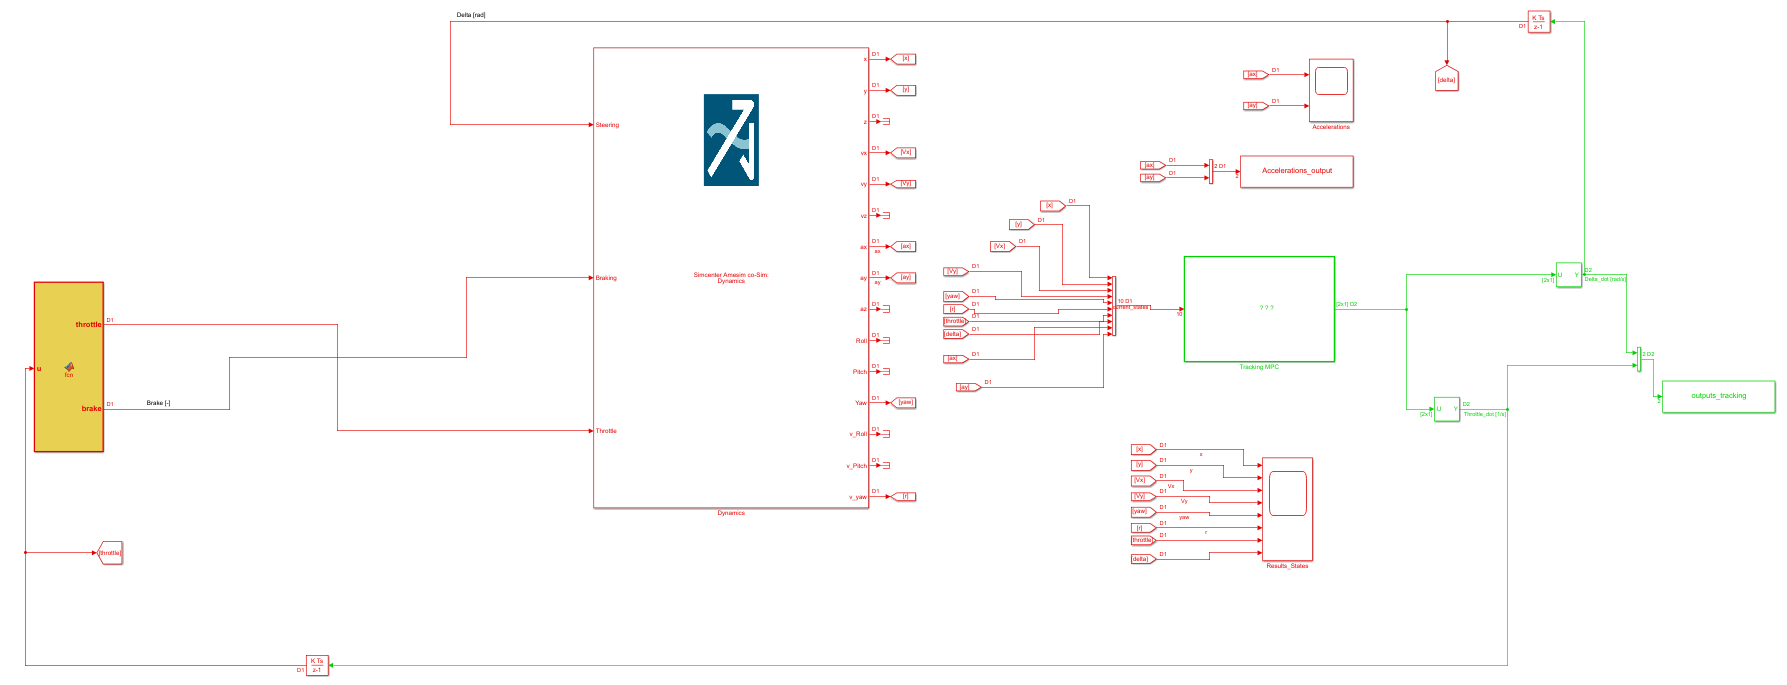
\includegraphics[width=1.1\textwidth]{simulink_model.PNG}
	\caption{This figure shows hows the tracking MPC is connected with the Amesim model using different sampling times. (red: $T_s: 0.01\hspace{1mm}s$ and green: $T_{MPC}:0.1\hspace{1mm}s$)}	
	\label{fig:simulink_model}
\end{figure}

The three inputs to the Amesim model (largest block)  in Figure \ref{fig:simulink_model} are $\delta_s$, $t_r$ and $braking$ but the control outputs of Eq. (\ref{opt:tracking}) give $\dot{t}_r$ and $\dot{\delta_s}$. Therefore 'Forward Euler integration' blocks are introduced using for $0.1\hspace{1mm}s$ the control outputs of Eq. (\ref{opt:tracking}) in order to calculate every $0.01\hspace{1mm}s$ the inputs for the Amesim model. The throttle of the bicycle model can theoretically become positive and negative. These two states were separated and feeded to the Amesim model as throttling or braking. 


\subsection{Tracking results} 
\label{s:tracking_results}

In this section the results of the tracking MPC are presented. For a full overview of the results, reference is made to Appendix \ref{app:D}. Figure \ref{fig:xy_mpc} shows that the tracking of the path (blue) of the reference (red) is done with an accuracy of $10^{-3}$. 

\begin{figure}[h!]
	\centering
	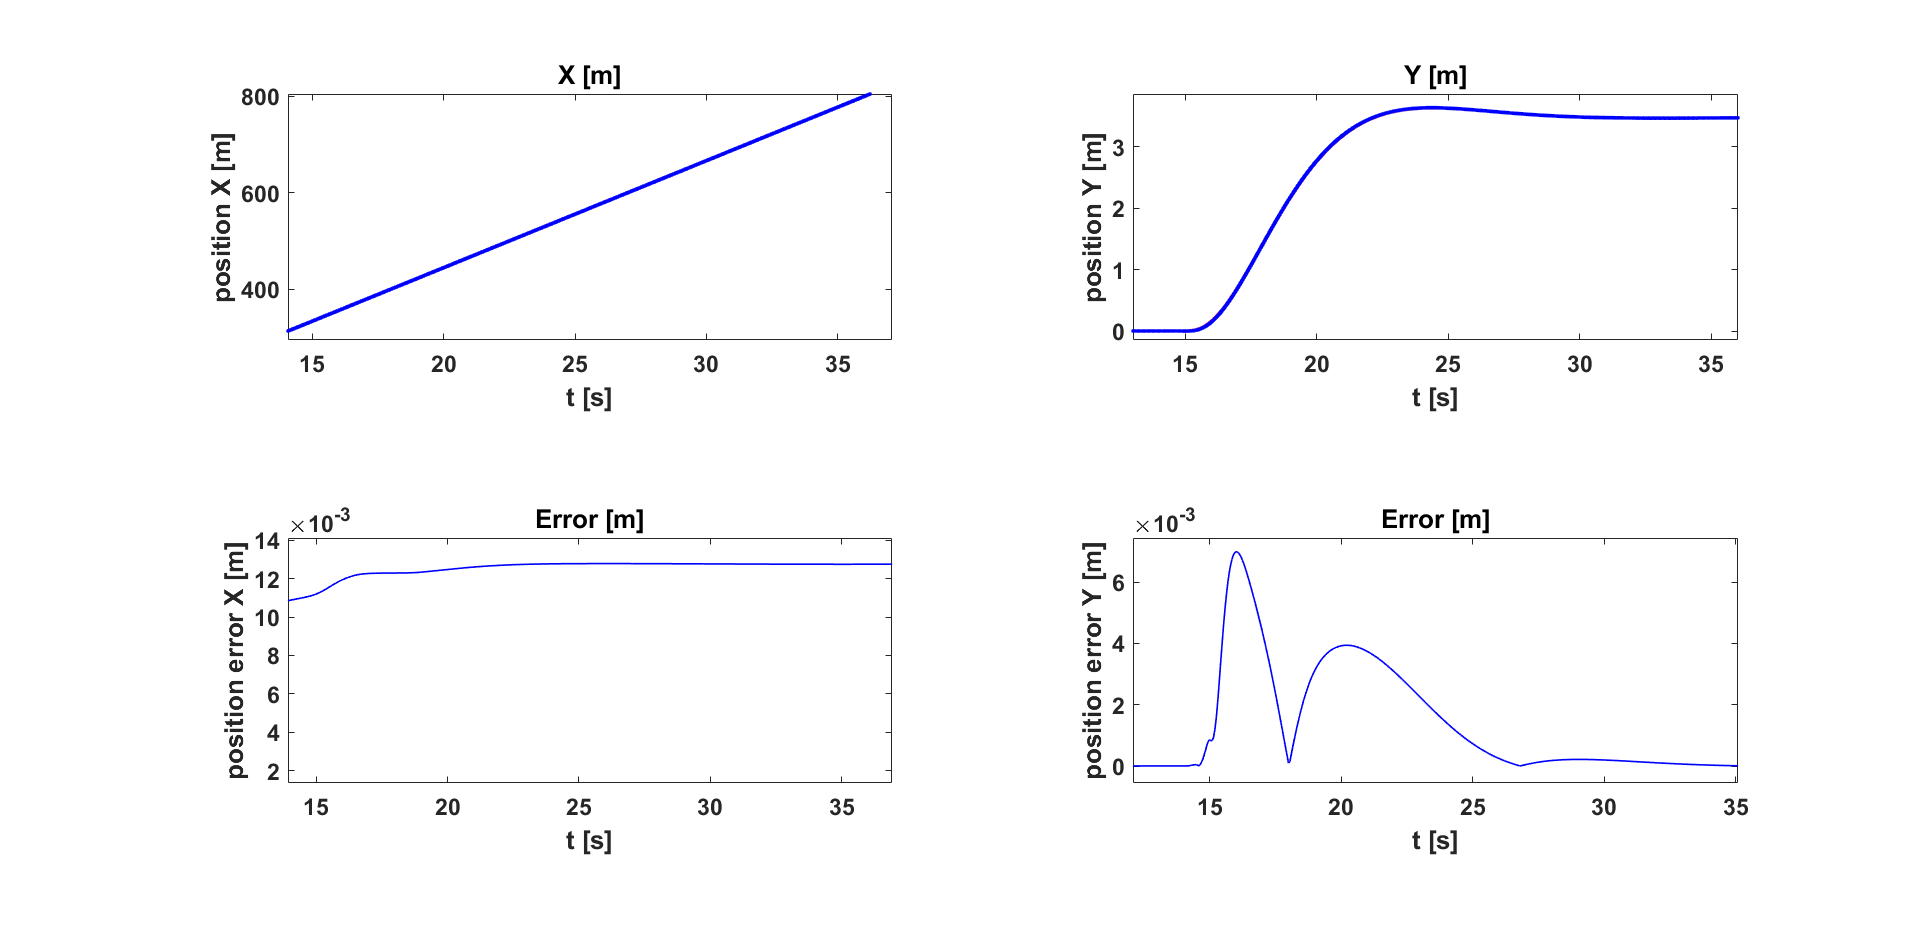
\includegraphics[width=1.1\textwidth]{2xy_N50_TMPC 0.1_Tf40.PNG}
	\caption{This figure shows the tracking result of the reference (red) by the Amesim model (blue).}	
	\label{fig:xy_mpc}
\end{figure}

During the analysing of the results it was concluded that the important signals were followed sufficiently well to be able to use the tracking MPC in the learning configuration of Figure \ref{fig:complex_learning}. However there were also differences seen between the reference and the followed trajectory. This justifies the reasoning that not all states have to be included in the error function of Eq. (\ref{opt:tracking}), because tracking all states accurate will give worse results due to inherent vehicle model mismatch. The first difference is that the Amesim model needs a bigger steerwheelangle than was predicted by the reference. Also the amount of throttle needed to drive forward at a constant speed is slightly different because of a more complete way of aerodynamic resistance modelled by the Amesim model in comparison to Eq. (\ref{eq:bicycle_Fdrag}) used by the bicycle model.\\
Another observation is that the lateral jerk and first derivative of the steerwheelangle display less high peaks than the reference. Also when there is closely zoomed in on the longitudinal jerk around $15\hspace{1mm}s$, which coincides with the start of the lane change and $22\hspace{1mm}s$ which is more at the end, nervous behaviour of the longitudinal jerk is witnessed. Around $15\hspace{1mm}s$ a bump in the reference of the throttle can be seen because that is the point where straight driving at constant speeds ends and the reference is from there on  produced by a solution of Eq. (\ref{opt:basic_opti_w}). The influence on $v_x$ and $a_x$ is however marginal. Further it is worth to note that the jerks don't come directly from the Amesim model but the signal is post-processed by numerical differentiation. \\

To be able to generate adequately smooth jerk signals, it was necessary to include smooth inputs of throttle and steerwheelangle. Figure \ref{fig:old_inputs} shows oscillating behaviour of the lateral jerk when not the first derivative of throttle and steerwheelangle are used as control outputs of Eq. (\ref{opt:tracking}). That the jerk signal is dependent on the first derivative of throttle and steeringwheelangle is a logical result, because also in the analytical jerk equations of the non-linear bicycle model (Appendix \ref{app:A}) these variables were embedded.\footnote{For the results of Figure \ref{fig:old_inputs}, no straight driving reference path is added. The lane change directly starts at $time = 0.0$.}

\begin{figure}[h!]
	\centering
	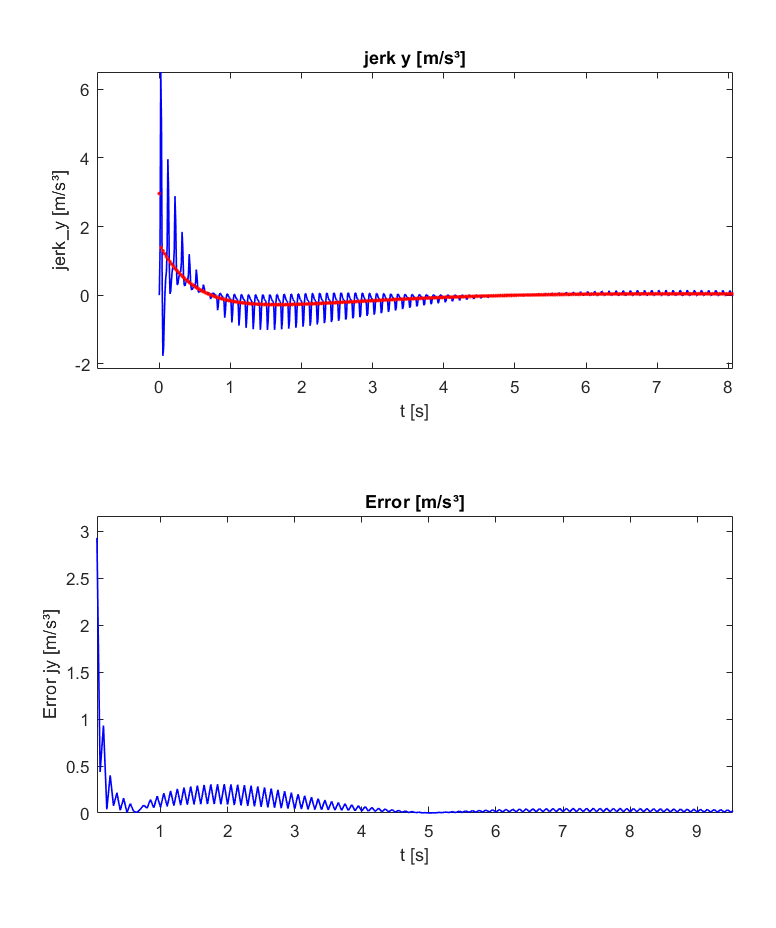
\includegraphics[width=0.8\textwidth]{9jerks_N50_TMPC 0.1_Tf22.5_adjusted.PNG}
	\caption{This figure shows the obtained oscillating signals for the jerk when a piecewise signal of $\delta_s$ and $t_r$ is applied.}	
	\label{fig:old_inputs}
\end{figure}

\section{Learning results with the Amesim model}
\label{s:complex_learning_results}
Diagram \ref{fig:complex_learning} shows in blue the observed path that is generated out of Eq. (\ref{opt:basic_opti_w}) with known weights whereafter the path based on a bicycle model is tracked by a tracking MPC to get the kinematic signals of the $15$ dof Amesim model. From this $\bm{F}^*(\bm{r})$ is calculated which stays constant during whole the learning process.\\

The learning loop shown in red in diagram \ref{fig:complex_learning} starts at the lane change planner, where Eq. (\ref{opt:basic_opti_w}) is called with an initial guess of the weights an all-one vector. After the planned path is outputted, tracked\footnote{The first $10 \hspace{1mm}s$ of the tracked Amesim signal is removed. The remaining maneuver consists of $5 \hspace{1mm}s$ straight driving before doing the actual lane change.} and the associated feature vector $\bm{F}(\bm{r})$ is calculated, it is checked if the two feature vectors match accurate enough in the convergence block. If this is not the case, the difference of the features is taken as an estimate for $\pdv{\bm{F}}{\bm{\theta}}$ and used in the RPROP algorithm in order to generate a new planned path by calling Eq. (\ref{opt:basic_opti_w}). \\

Four simulations are conducted with respectively one, two, three and five datasets. Table \ref{tab:datasets_overview} shows which longitudinal speed is driven at the begin of the lane change ($V_{0}$) and the desired lateral displacement $(L)$. As is noted before in Chapter $\ref{cha:Learning_algorithm}$, if only the start speed is varied, the lateral feature values stay the same and the longitudinal features stay very small. This means that these datasets are seen as almost the same when learning. When the lateral desired displacement is varied, this gives a clear difference in the lateral feature values. An overview of the different features of the individual datasets is given in table \ref{tab:indi_features}. \footnote{In the calculation of the feature values the $5 \hspace{1mm}s$ straight driving before the lane change is included. This contributes to a higher value for feature number six.} 



\begin{table}[h!]
	\centering
	\begin{tabular}{@{}llllr@{}} \toprule
		1 Dataset    & 2 Datasets & 3 Datasets & 5 Datasets\\ \midrule
     $V0:22.22 - L:3.47$  & $V0:22.22 - L:3.47$    & $V0:22.22 - L:3.47$ & $V0:22.22 - L:3.47$		\\
           			 & $V0:25.00 - L:6.94$      & $V0:25.00 - L:6.94$    & $V0:25.00 - L:6.94$  \\
	        		 &        & $V0:27.78 - L:3.47$ & $V0:27.78 - L:3.47$      \\ 
&	&	&$V0:22.22 - L:6.94$	\\
&	&	&$V0:25.00 - L:3.47$	\\\bottomrule
	\end{tabular}
	\caption{This table shows which lane changes were used during the four different simulations.}
	\label{tab:datasets_overview}
\end{table} 


\begin{table}[h!]
	\centering
	\begin{tabular}{@{}llllllr@{}} \toprule
	\textbf{Feature}     & V022.22 - L3.47 & 	V022.22 - L6.94 & V025.00 - L3.47 &	V025.00 - L6.94 & V027.78 - L3.47\\ \midrule
		Nr.1       		  &5.18e-07 &7.20e-06  	& 3.88e-07     & 5.97e-06  & 4.01e-07\\
		Nr.2              & 0.38 &1.50&	     0.38      & 1.51    &       0.38       \\
		Nr.3              & 12.29e-05&14.53e-05	& 1.67e-05 &	7.23e-05 &5.37e-06\\
		Nr.4              & 0.51 &2.06&	         0.52 &          2.09   &   0.52    \\
		Nr.5              & 9.50e-06&4.42e-05   & 1.66e-05      & 7.08e-05  & 3.71e-05       \\
		Nr.6              & 91.25 &	364.99      &	91.25	&364.97       & 91.25       \\ \bottomrule
	\end{tabular}
	\caption{This table shows the different features for the individual datasets used during simulation.}
	\label{tab:indi_features}
\end{table} 

The weights learned for the four different simulations is presented in table \ref{tab:complex_learning_weights}\footnote{The weights that come of the simulations are scaled so that the second weight equals $5.0$.} and $\bm{f}_{rel}$ at convergence is given in table \ref{tab:complex_frel}.   $\bm{f}_{rel}$ displays the matching of the averaged learned feature values with the observed one. Convergence for the four simulations is reached after 28 iterations. The convergence criteria used is matching the lateral features (2,4,6) with a tolerance of $10^{-3}$.\\

\begin{table}[h!]
	\centering
	\begin{tabular}{@{}llllr@{}} \toprule
		\textbf{Weight}   & 1 Dataset    & 2 Datasets     & 3 Datasets & 5 Datasets\\ \midrule
		Nr.1       		  &33.4230       & 5.2294       & 3.9036 & 4.2995 		\\
		Nr.2              & 5.0000         & 5.0000          & 5.0000 &5.0000      \\
		Nr.3              & 2.8662e-06     & 1.0636      & 1.9803   &3.4930   \\
		Nr.4              & 6.0018           & 6.0018            &   6.0018&6.0278     \\
		Nr.5              & 4.4445     & 1.2705      & 1.1869 &1.5694      \\
		Nr.6              & 2.0011        & 2.0011         & 2.0011 & 2.0044     \\ \bottomrule
	\end{tabular}
	\caption{This table shows the weights learned for the different simulations that start from an all one vector and uses as chosen weights $\bigl[ \begin{smallmatrix} 4.0,&5.0,&1.0,&6.0,&1.0,&2.0\end{smallmatrix}\bigr]$.}
	\label{tab:complex_learning_weights}
\end{table}

\begin{table}[h!]
	\centering
	\begin{tabular}{@{}llllr@{}} \toprule
		$\bm{f}_{rel}$   & 1 Dataset    & 2 Datasets & 3 Datasets&5 Datasets\\ \midrule
		Nr.1       		  &1.1315        & 1.0097       & 0.9643&0.9677		\\
		Nr.2              & 1.0000         & 1.0002     & 1.0003&1.0005        \\
		Nr.3              & 0.2865     & 0.4496     	& 0.4867  &0.9957     \\
		Nr.4              & 1.0000           & 1.0002   &   1.0002 &0.9993     \\
		Nr.5              & 1.0718     & 1.0030         & 0.9937 &0.9772       \\
		Nr.6              & 1.0000        & 1.0000      & 1.0000 &1.0000    \\ \bottomrule
	\end{tabular}
	\caption{This table shows the final values of $\bm{f}_{rel}$.}
	\label{tab:complex_frel}
\end{table}

Out of table \ref{tab:complex_learning_weights} and \ref{tab:complex_frel} it is concluded that the lateral chosen weights are found back and an accurate match of the lateral features is achieved. It is observed that also the longitudinal weights will come closer to their chosen value and give a better match for the longitudinal feature values, when more observed lane changes are included in the learning.

Figure \ref{fig:complex_path} presents the observed paths, the initial solution when the weight vector is chosen equal to an all-one vector and the learned solution when $2$ datasets are used. Figure \ref{fig:complex_path_error} shows the error made between the observed and learned path which is of order of size of $10^{-4}$. All the resulting kinematic signals are displayed in Appendix \ref{app:E}.

\begin{figure}[h!]
	\centering
	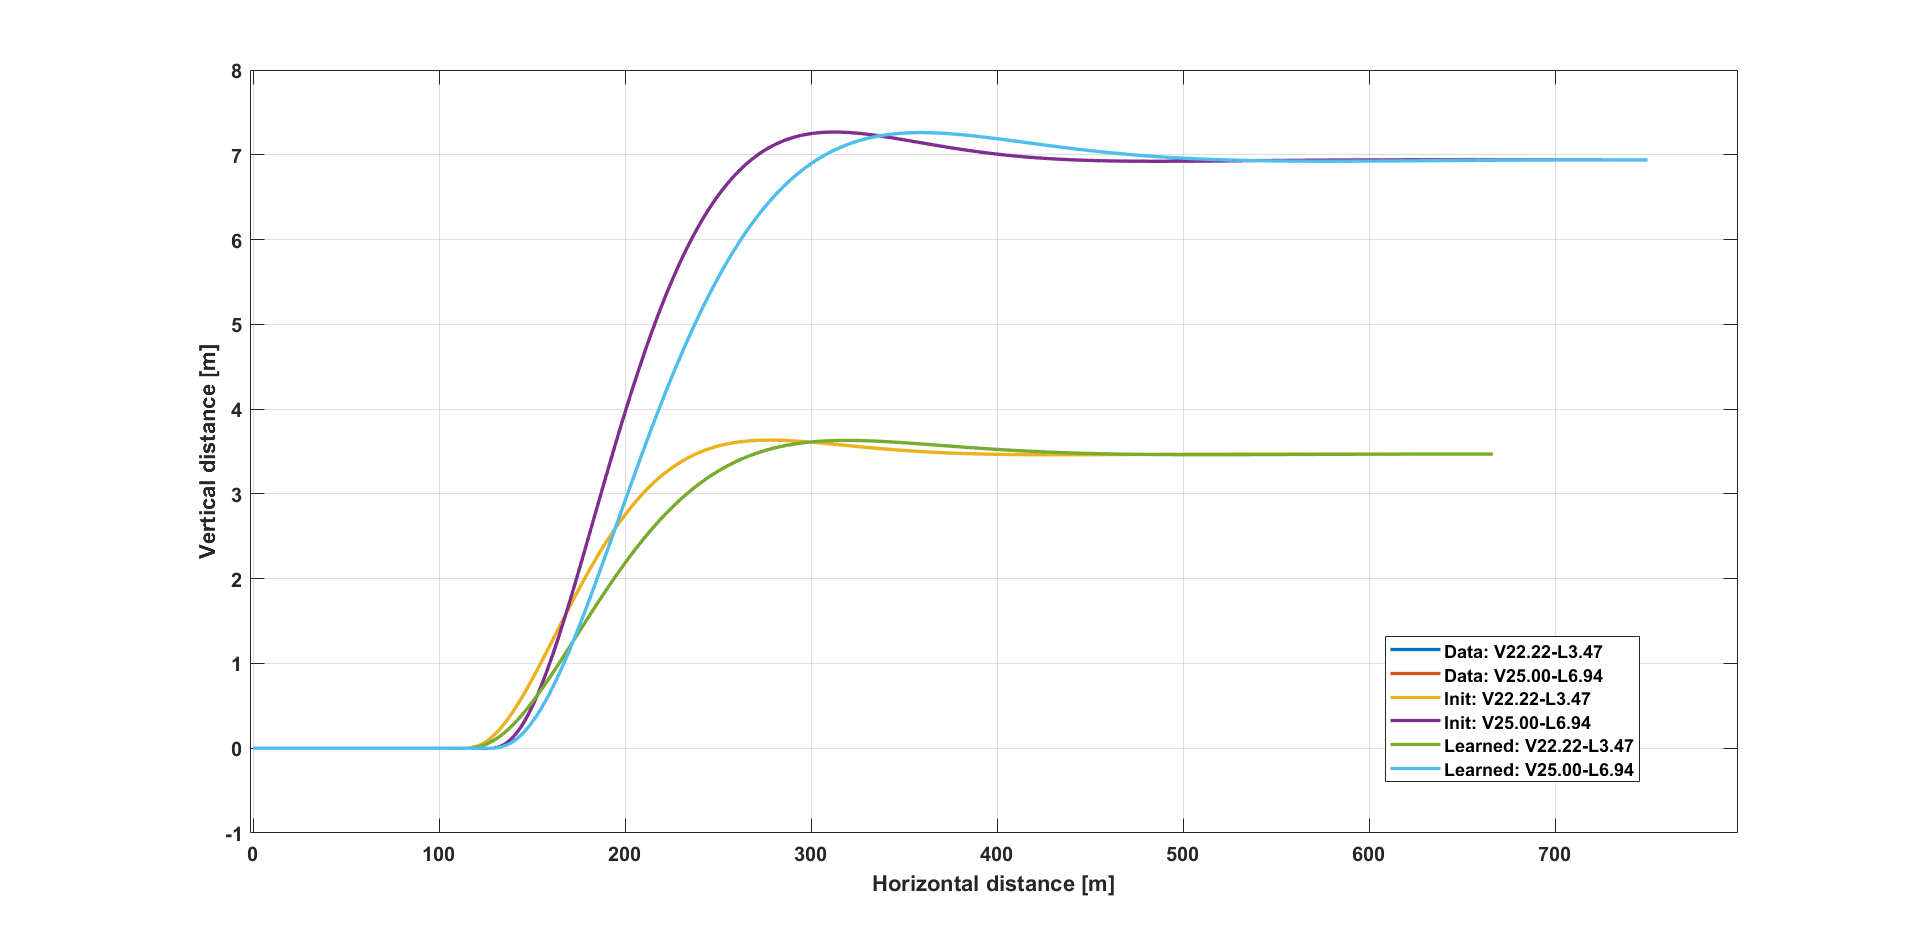
\includegraphics[width=1.1\textwidth]{2path_N1000IT28.PNG}
	\caption{This Figure shows the observed paths, the initial solution retrieved with as weights an all one vector and the learned solution.}	
	\label{fig:complex_path}
\end{figure}

\begin{figure}[h!]
	\centering
	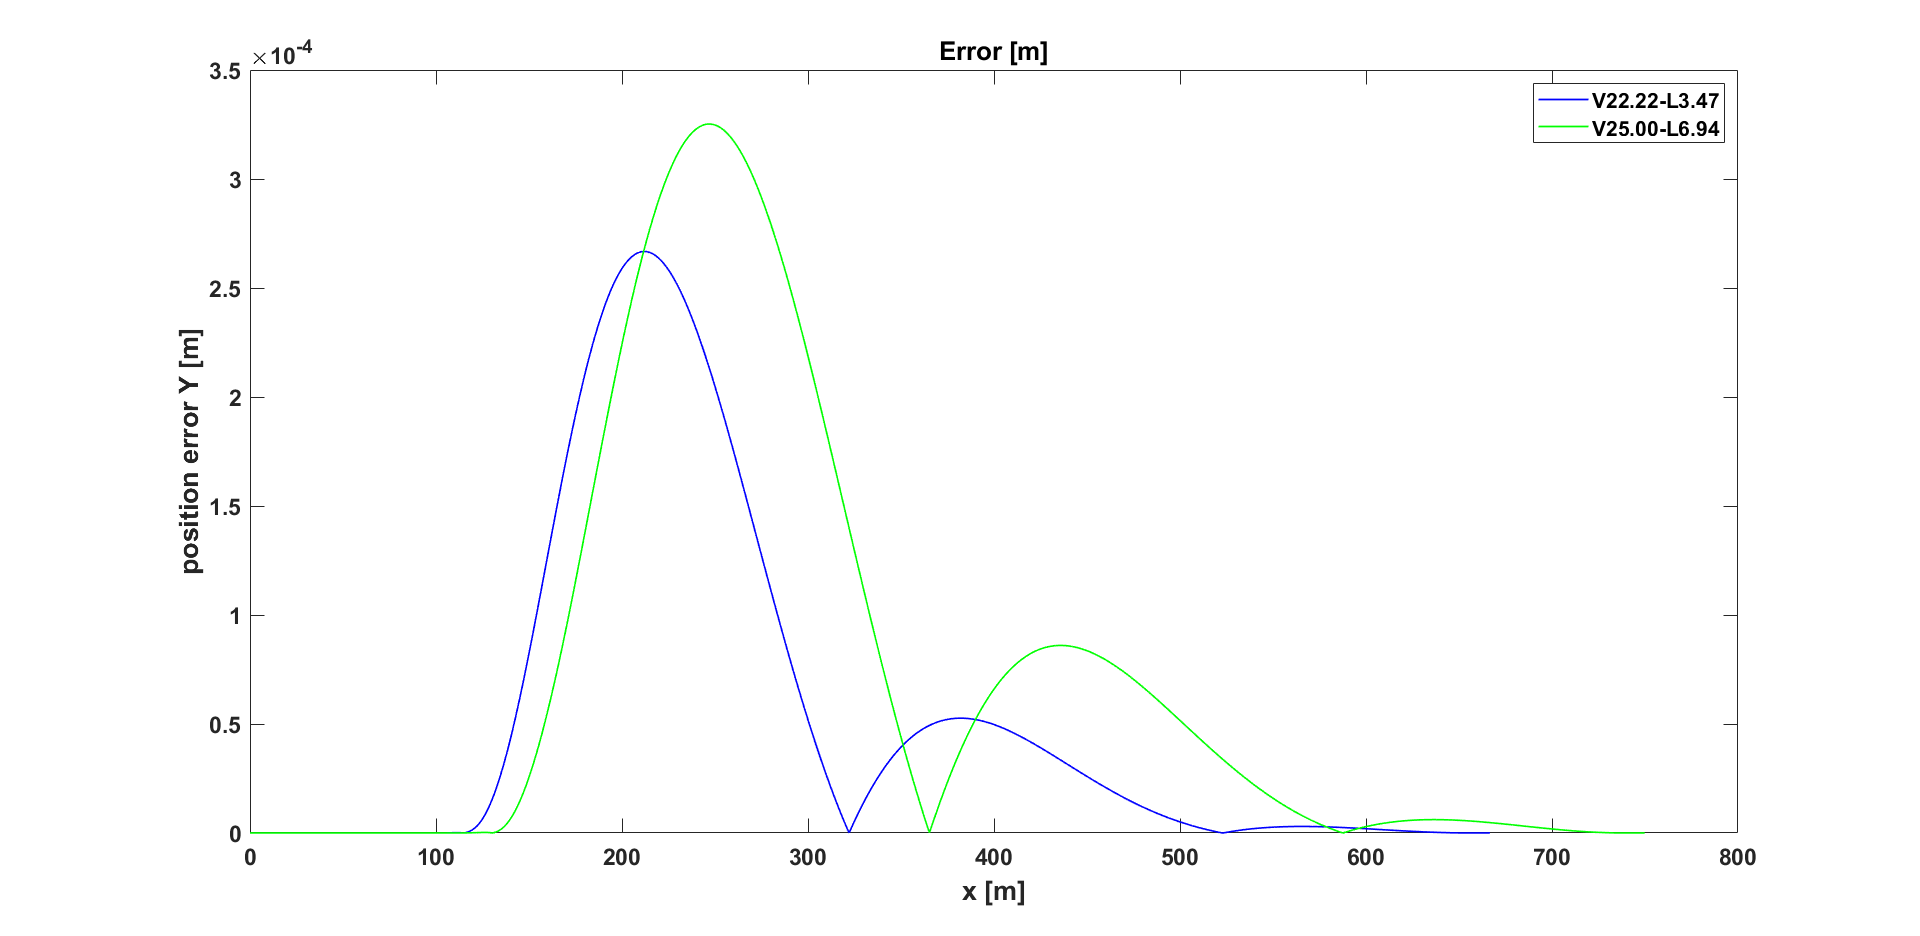
\includegraphics[width=1.1\textwidth]{error learned path.PNG}
	\caption{This Figure shows the error made between the observed and learned paths.}	
	\label{fig:complex_path_error}
\end{figure}

Figure \ref{fig:complex_convergence} shows the convergence of $\bm{f}_{rel}$ towards one during the learning iterations. Except for the longitudinal jerk (feature $3$) all the feature values converge towards the observed ones.

\begin{figure}[h!]
	\centering
	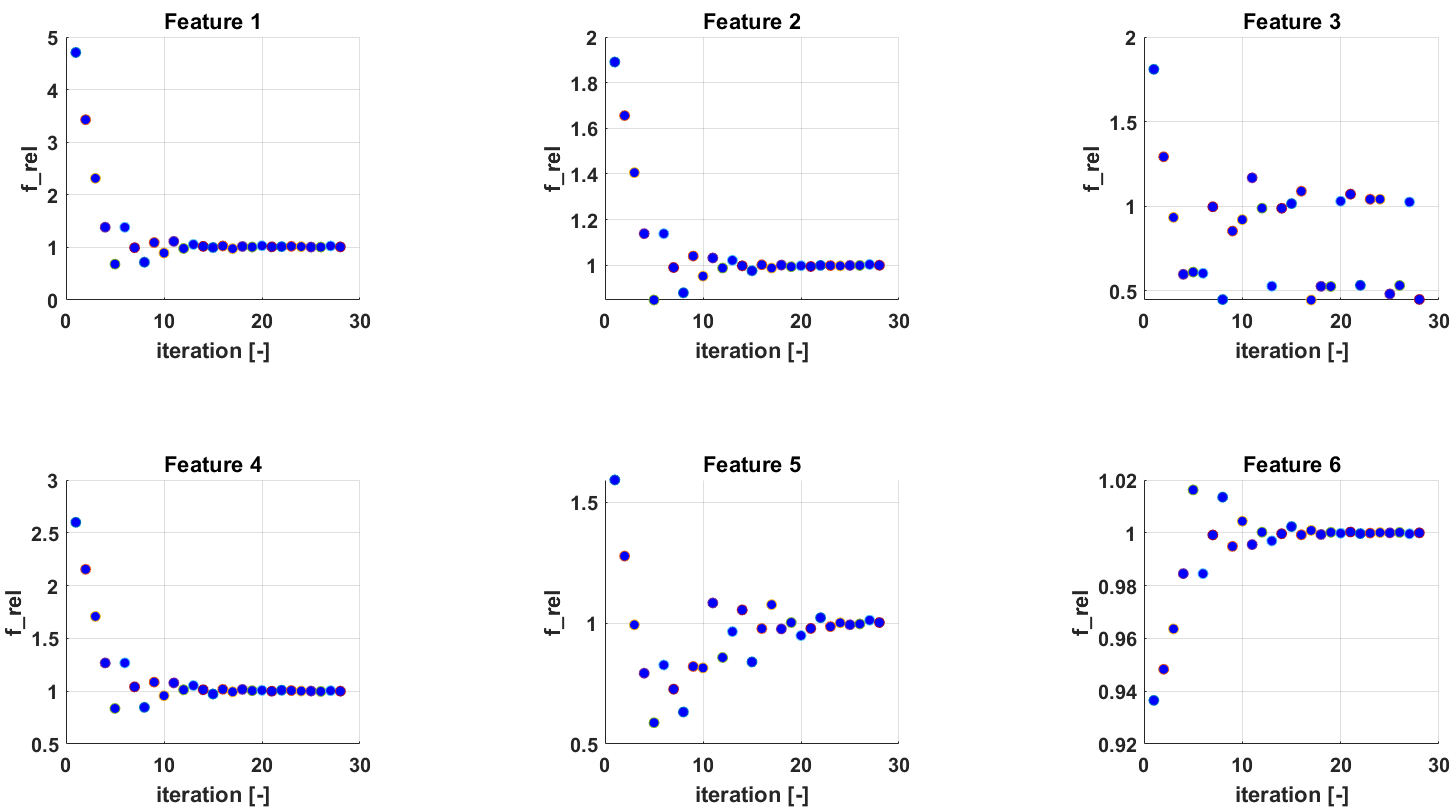
\includegraphics[width=1.1\textwidth]{12frel.PNG}
	\caption{This Figure shows $\bm{f}_{rel}$ during the learning iterations.}	
	\label{fig:complex_convergence}
\end{figure}

From the retrieved $\bm{f}_{rel}$ of table \ref{tab:complex_frel} and in Figure \ref{fig:complex_convergence}, the feature value for the longitudinal jerk (Nr. $3$), jumps out for its bad feature matching behaviour. ($...$ when five datasets are used) A reason for this is as discussed in \ref{s:tracking_results}, bad quality of the jerk data which contributes to a worsen learning. The jerk during the lane change can be seen in Figure \ref{fig:complex_jerk}. At time zero the longitudinal behaviour is still not fully stabilized and at second $5$ the lane change starts.

\begin{figure}[h!]
	\centering
	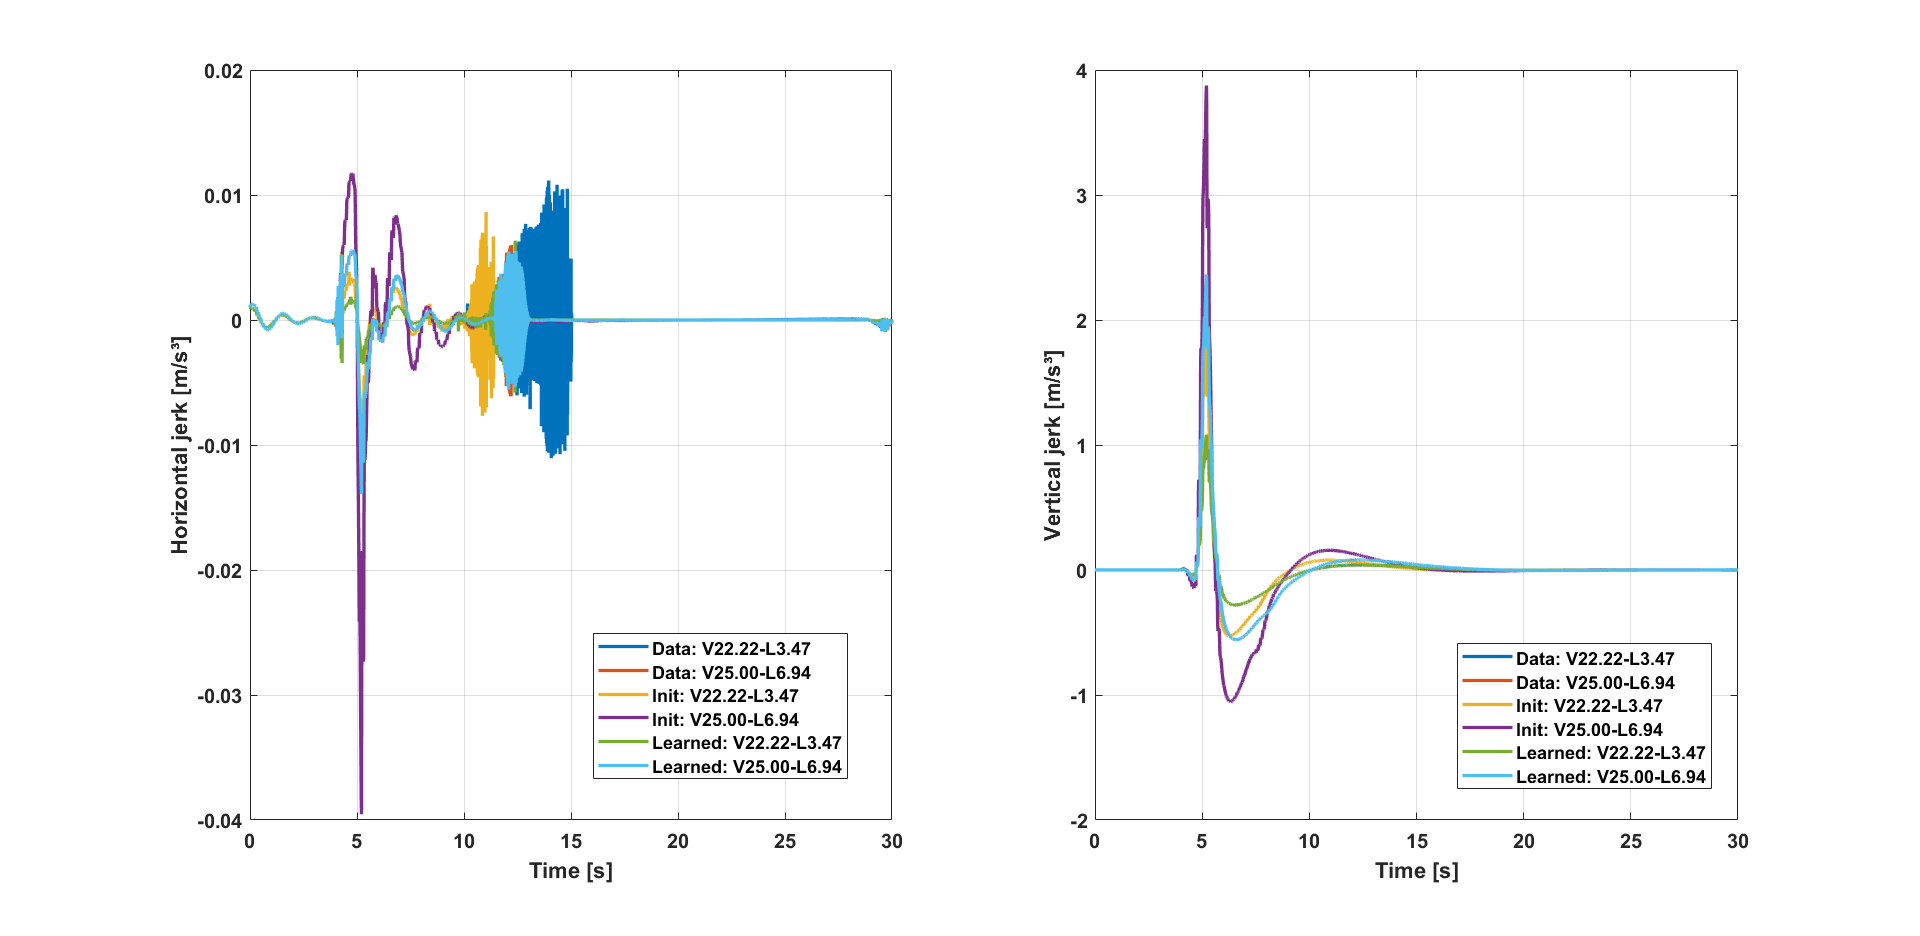
\includegraphics[width=1.1\textwidth]{7JX_JY_N1000IT28.PNG}
	\caption{This Figure shows the observed jerk signals, the initial solution retrieved with as weights an all one vector and the learned solution.}	
	\label{fig:complex_jerk}
\end{figure}
 \newpage                                
\section{Conclusion}
In this chapter the learning of driver specific comfort parameters with a realistic $15$ dof Amesim model was discussed. The flow of the different steps of the learning process and how the Amesim model would be embedded, was looked into. The question posed was: "Is it possible to find back the underlying comfort weights when the gradient $\pdv{\bm{F}}{\bm{\theta}}$ is estimated by $ \bm{F}_{obs} - \bm{F}(\bm{r}_{expected})$". \\

First the formulation of the used tracking MPC was presented and its tracking performance evaluated. The results are that tracking of the planned path was possible to an accuracy of $10^{-3}$ and also the other important features $a_y$ and $j_y$ could be tracked to a satisfying accuracy as can be seen in Appendix \ref{app:D}. However $\delta_s$, $t_r$ in steady-state and the peaks of $\dot{\delta_s}$ and $j_y$, gave a difference with the reference when the path generated by the non-linear bicycle model is being accurate tracked. Next a notion was made about the bad quality of the obtained longitudinal jerk signal. Eventually it was stated that only a smooth signal for the lateral jerk can be retrieved when the input signals are at least of first order. \\

When the tracking MPC was validated the learning results with the Amesim model were discussed. Four simulations were conducted with a different amount of observed lane changes. Out of the results it could be concluded that every time there is a good convergence found for $\bm{f}_{rel}$ and the chosen lateral weights are found back. When more observed lane changes are included during the learning also the results for the longitudinal weights improve. \\
Only the convergence of the longitudinal jerk stayed deficient, which is due to bad quality of the longitudinal jerk data that was used to learn the weights of.



%%% Local Variables: 
%%% mode: latex
%%% TeX-master: "thesis"
%%% End: 
\chapter{Enhanced weighting factor update}
\label{cha:Enhancement}

This chapters proposes a theoretical alternative for updating $\bm{\theta}^k$ during the learning iterations. The previous method made use of the gradient approximation $\bm{F}_{obs} - \bm{F}(\bm{r}_{expected})$ embedded in a gradient descent formulation and the step size determined by the RPROP algorithm. The method proposed here, calculates $\bm{\theta}^{k+1}$ based on an unconstrained optimization.\\

The chapter is structured as follows. First, the formulation of the method to update the weight factor is discussed in section \ref{s:formulation_enh}. Afterwards a discussion follows in section \ref{s:discussion_enh} and finally a conclusion is given in section \ref{s:conclusion_enh}
\section{Formulation}\label{s:formulation_enh}
The goal of the learning algorithm is to find a set of weight factors $\bm{\theta}$ that will match $\bm{F}$ as closely as possible to $\bm{F}_{obs}$. From this naturally the unconstrained minimization of the error function as defined by Eq. (\ref{eq:obj_enh}) follows.

\begin{multline}\label{eq:obj_enh}
E(\bm{\theta}) = |f_{obs,1} - f_1(\bm{\theta})|+|f_{obs,2} - f_2(\bm{\theta})|+|f_{obs,3} - f_3(\bm{\theta})|\\
+|f_{obs,4} - f_4(\bm{\theta})|+|f_{obs,5} - f_5(\bm{\theta})|+|f_{obs,6} - f_6(\bm{\theta})|
\end{multline}

However $\bm{F}(\bm{\theta})$ is not knowns analytically and therefore should be approximated by a second order multivariate Taylor expansion as described by \ref{eq:taylor}. The gradient and the hessian are respectively given by Eq. (\ref{eq:Grad}) and Eq. (\ref{eq:Hess}). The solution of the minimization of Eq. (\ref{eq:obj_enh}) is taken as $\bm{\theta}^{k+1}$.

\begin{equation}\label{eq:taylor}
	f_i({\bm{\theta}}) \approx f_i(\bm{\theta}^k) + \nabla f_i(\bm{\theta})^T|_{\bm{\theta} = \bm{\theta}^k}\cdot (\bm{\theta} - \bm{\theta}^k) + \frac{1}{2}(\bm{\theta} - \bm{\theta}^k)^T\cdot \bm{H}_i(\bm{\theta})|_{\bm{\theta} = \bm{\theta}^k}\cdot(\bm{\theta} - \bm{\theta}^k)
\end{equation}
\[\forall i,k \in \mathbb{N}\]

\begin{equation}\label{eq:Grad}
\centering
\nabla f_i(\bm{\theta})^T = 
\begin{bmatrix}
\pdv{f_i}{\theta_1} & \pdv{f_i}{\theta_2} & \pdv{f_i}{\theta_3} & \pdv{f_i}{\theta_4} &\pdv{f_i}{\theta_5} & \pdv{f_i}{\theta_5} & \pdv{f_i}{\theta_6}
\end{bmatrix}
\end{equation}

\begin{equation}\label{eq:Hess}
\centering
\bm{H}_i(\bm{\theta}) = 
\begin{bmatrix}

 \pdv[2]{f_i}{\theta_1} & \pdv{f_i}{\theta_1}{\theta_2}& \pdv{f_i}{\theta_1}{\theta_3}& \pdv{f_i}{\theta_1}{\theta_4}& \pdv{f_i}{\theta_1}{\theta_5}& \pdv{f_i}{\theta_1}{\theta_6}\\
 
  \pdv{f_i}{\theta_2}{\theta_1}&\pdv[2]{f_i}{\theta_2} & \pdv{f_i}{\theta_2}{\theta_3}& \pdv{f_i}{\theta_2}{\theta_4}&\pdv{f_i}{\theta_2}{\theta_5}&\pdv{f_i}{\theta_2}{\theta_6}\\
  
  \pdv{f_i}{\theta_3}{\theta_1}&\pdv{f_i}{\theta_3}{\theta_2}&\pdv[2]{f_i}{\theta_3} &  \pdv{f_i}{\theta_3}{\theta_4}&\pdv{f_i}{\theta_3}{\theta_5}&\pdv{f_i}{\theta_3}{\theta_6}\\
  
  \pdv{f_i}{\theta_4}{\theta_1}&\pdv{f_i}{\theta_4}{\theta_2} &  \pdv{f_i}{\theta_4}{\theta_3}&\pdv[2]{f_i}{\theta_4}&\pdv{f_i}{\theta_4}{\theta_5}&\pdv{f_i}{\theta_4}{\theta_6}\\
  
  \pdv{f_i}{\theta_5}{\theta_1}&\pdv{f_i}{\theta_5}{\theta_2} &  \pdv{f_i}{\theta_5}{\theta_3}&\pdv{f_i}{\theta_5}{\theta_4}&\pdv[2]{f_i}{\theta_5}&\pdv{f_i}{\theta_5}{\theta_6}\\
  
  \pdv{f_i}{\theta_6}{\theta_1}&\pdv{f_i}{\theta_6}{\theta_2} &  \pdv{f_i}{\theta_6}{\theta_3}&\pdv{f_i}{\theta_6}{\theta_4}&\pdv{f_i}{\theta_6}{\theta_5}&\pdv[2]{f_i}{\theta_6}

\end{bmatrix}
\end{equation}\\

In order to investigate the local behaviour of a certain feature value $f_i$ in function of $\bm{\theta}$, the weight factors are slightly varied around $f_i(\bm{\theta}^k)$. This is done as described by Eq. $(\ref{eq:theta_a})$ for weight $\theta_j$.

\begin{subequations}\label{eq:theta_a}
\begin{equation}\label{eq:tplus}
	\theta^{k,+}_j = \theta^k_j + \Delta \theta
\end{equation} 

\begin{equation}\label{eq:tmin}
	\theta^{k,-}_j = \theta^k_j - \Delta \theta
\end{equation}
\end{subequations}

\begin{subequations}\label{eq:diff_enh}
	\begin{equation}\label{eq:1azer}
	\pdv{f_i}{\theta^k_j} = \frac{f_i|_{\theta^{k,+}_j}-f_i|_{\theta^{k,-}_j}}{2\Delta \theta}
	\end{equation}
	\begin{equation}
	\pdv[2]{f_i}{\theta_{k,j}} = \frac{f_i|_{\theta^{k,+}_j}-2f_i|_{\theta^k_j}+f_i|_{\theta^{k,-}_j}}{\Delta \theta^2}
	\end{equation}
\end{subequations}

For every evaluation of $f_i$, Eq. (\ref{opt:basic_opti_w}) is called and outputs six feature values. The solution of the optimization variables and lambda multipliers are knowns for $\bm{\theta}^k$ from the previous iteration and is used as initial guess which only difference with a very small value $\Delta \theta$ for a certain weight. It is expected that when the SQP method is used, that exploits that very good initial guess, convergence is fast reached.\\
Eq. (\ref{opt:basic_opti_w}) is called $12$ times in order to estimate the $6$ gradients of the different features and the diagonals of the six Hessians, when making use of the previous solution $\bm{F}(\bm{\theta}^k)$. \\

The hessian is assumed to be symmetrical, which means that only the cross derivates above the diagonal have to be calculated. The derivation of the of the cross derivatives can become quite complex, but an intuitive approach relies on the subsequent use of one-dimensional finite-difference discretization as in the example given by Eq. (\ref{eq:book}). This formulation is second order when the mesh is equidistant, orthogonal and with p, and z the mesh-point numbering \cite{Meyers}

\begin{equation}\label{eq:book}
	\pdv{\phi}{x}{y} \approx \frac{\pdv{\phi}{y}|_{p+1,z} - \pdv{\phi}{y}|_{p-1,z}}{2 \Delta x}.
\end{equation}

\[p,z \in \mathbb{N}\]

This translates with the use of Eq. (\ref{eq:1azer}) into Eq. (\ref{eq:1azerty}) 

\begin{equation}\label{eq:1azerty}
\pdv{f_i}{\theta^{k}_p}{\theta^{k}_z} \approx \frac{f_i|_{\theta^{k,+}_p,\theta^{k,+}_z} - f_i|_{\theta^{k,+}_p,\theta^{k,-}_z} - f_i|_{\theta^{k,-}_p,\theta^{k,+}_z}+f_i|_{\theta^{k,-}_p,\theta^{k,-}_z}}{4(\Delta \theta)^2}.
\end{equation}

The conditions of an equidistant mesh is fulfilled when $\Delta \theta$ is taken the same for the different weights. The condition of an orthogonal mesh is automatically satisfied because a weight factor can be changed independently of the other weight factors. \\
Because for the calculation of every cross derivative Eq. (\ref{opt:basic_opti_w}) is called $4$ times, this means the in order to calculate the full Hessian a total of $72$ evaluations of Eq. (\ref{opt:basic_opti_w}) are needed. After this, the error function of Eq. (\ref{eq:obj_enh}) can be minimized. 




%EI had an idea about substituting  the gradient update by an update based on an optimization. In short I wanted during solving investigate the relation ofdF/dθ by varyingθ by a small value and solve the very similar solution again in order to get numerical estimates of the first derivative and the second derivative to be able to fill that in the second order taylor approximation forF(θ). After that I can minimize|F_obs-F(θ)| by a standard L1 fitting and this updates my new weights. This was just an idea I had and I didn’t had the time to look if it is feasible.

\section{Discussion} \label{s:discussion_enh}
Because 


Have to check if it is feasible to evaluate the opti zo vaak
ook kijken of hessian niet kan benaderen
of enkel naar eerste orde kijken
approximations for the hessian
\section{Conclusion}\label{s:conclusion_enh}

%\begin{algorithm}[H]
%	\SetAlgoLined
%	\KwResult{$\bm{\theta}_{opti}$ }
%	initialization: \\
%	$\bm{\theta} = [1,1,...,1,1] $\\
%	$\bm{\tilde{f}} = \frac{1}{m} \sum_{i=1}^{m}\bm{f}(\bm{r}_{obs,i}) $ \;
%	\While{Not converged}{
%		\For{i = 1...m}{	
%			$\smash{\displaystyle\min_{r_{exp}}} \hspace{3 mm} \bm{\theta}^T\cdot\bm{f}(\bm{r}_{exp})$ \;
%			\vspace{2 mm} 
%			constraints: \\
%			\hspace{5 mm}$vehicle\_model$\;
%			\hspace{5 mm}$begin = initial(observed_i)$\;
%			\hspace{5 mm}$end = [y = lane\_distance_{i}, vy = 0, ay = 0, jy = 0]$\;
%			\hspace{5 mm}$physical\_boundaries\_vehicle$\;		
%		} \\
%		
%		$\bm{f}_{obtained} = \frac{1}{m} \sum_{i=1}^{m}\bm{f}(\bm{r}_{exp,i})$ \;
%		$\Delta \bm{\theta} = \alpha\cdot(\bm{f}./\bm{\tilde{f}}-\bm{1})$\;
%		$\bm{\theta} = \bm{\theta} + \Delta \bm{\theta}$\;
%		\If{$\Delta \bm{\theta} \leq \epsilon$}{
%			$return \hspace{1 mm}\bm{\theta}$\;		
%		}
%	}
%	\caption{\textbf{Learning algorithm}}
%\end{algorithm}






















%%% Local Variables: 
%%% mode: latex
%%% TeX-master: "thesis"
%%% End: 

%\chapter{Validatie with expert driver data}
\label{cha:Validation}

Bespreek de validatie van de methode. Implementeer similaties in prescan.
Bespreek de verschillende software tools bij Siemens --> Amesim, simulink, prescan.
Hoe werken ze samen en hoe wordt de validatie precies gedaan? Wat zijn de resultaten?

Install amesim and write a chapter about how the dataset is generated. How is the amesim model defined etc. 

how accurate results are learned when the assumption on the observations is violated. (assumping generated by a comfort cost function)

The objective function of the MPC is slightly different of the one used in the learning algorithm. In the training set it was important to explain the observed data but it is known beforehand that the driver demonstrated a feasible path and wants to do a lane change. Now the situation is different and features that assess the environment are a necessity. For this reason the objective function of the learning algorithm is extended with features that handle collision avoidance and following distance. (Lane change behavior is influenced by the environment! )



%\begin{algorithm}[H]
%	\SetAlgoLined
%	\KwResult{$\bm{\theta}_{opti}$ }
%	initialization: \\
%	$\bm{\theta} = [1,1,...,1,1] $\\
%	$\bm{\tilde{f}} = \frac{1}{m} \sum_{i=1}^{m}\bm{f}(\bm{r}_{obs,i}) $ \;
%	\While{Not converged}{
%		\For{i = 1...m}{	
%			$\smash{\displaystyle\min_{r_{exp}}} \hspace{3 mm} \bm{\theta}^T\cdot\bm{f}(\bm{r}_{exp})$ \;
%			\vspace{2 mm} 
%			constraints: \\
%			\hspace{5 mm}$vehicle\_model$\;
%			\hspace{5 mm}$begin = initial(observed_i)$\;
%			\hspace{5 mm}$end = [y = lane\_distance_{i}, vy = 0, ay = 0, jy = 0]$\;
%			\hspace{5 mm}$physical\_boundaries\_vehicle$\;		
%		} \\
%		
%		$\bm{f}_{obtained} = \frac{1}{m} \sum_{i=1}^{m}\bm{f}(\bm{r}_{exp,i})$ \;
%		$\Delta \bm{\theta} = \alpha\cdot(\bm{f}./\bm{\tilde{f}}-\bm{1})$\;
%		$\bm{\theta} = \bm{\theta} + \Delta \bm{\theta}$\;
%		\If{$\Delta \bm{\theta} \leq \epsilon$}{
%			$return \hspace{1 mm}\bm{\theta}$\;		
%		}
%	}
%	\caption{\textbf{Learning algorithm}}
%\end{algorithm}




















\section{The First Topic of this Chapter}
\subsection{Item 1}
\subsubsection{Sub-item 1}


\subsubsection{Sub-item 2}


\subsection{Item 2}


\section{The Second Topic}


\section{Conclusion}

%%% Local Variables: 
%%% mode: latex
%%% TeX-master: "thesis"
%%% End: 

\chapter{Conclusion}
\label{cha:conclusion}
The contribution made with this thesis is the development of an algorithm based on inverse reinforced learning, that can learn driver specific experiences of comfort during a lane change and cast it into an objective function which explains observed data. \\
First a literature study was conducted in order to identify comfort during driving. Here it was found that smooth paths play an important role in contributing to the retrieved amount of comfort. Next, it was looked at the theoretical idea of feature based reinforcement learning. This was the starting point and the goal of this thesis was to scale this theoretical idea up to in practise useable models e.g. $15$ dof Amesim model.\\
In the following chapter, learning from ideal data was discussed. Here it was presented how ideal data was generated and validated and it was shown that the developed algorithm was able to accurately learn the chosen lateral weights that define the lane change maneuver. Thereby it was displayed that the estimation of the gradient $\pdv{\bm{F}_{diff}}{\bm{\theta}}$ by $ \bm{\tilde{F}} - \bm{F}(\bm{r}_{expected})$ can be used in order to converge towards the data feature vectors used.\\
Further, learning with a $15$ degrees of freedom vehicle model was discussed. For this matter a tracking MPC formulation was developed and it was shown that also here 
the algorithm was able to accurately learn the chosen lateral weights.\\
As last the theoretical idea was discussed how to replace the RPROP algorithm for updating the weight vector $\bm{\theta}$ by an optimized update. \\

This work has its practical usage in the avoidance of manual tuning of a comfort objective. When the objective is identified it can be used for path planning. Because this research is conducted together with Siemens, it is in line with the direction of their research and this thesis can be used to build further on.\\
The maneuver extensively discussed is a lane change maneuver. The only way that this is defined in Eq. \ref{opt:basic_opti_w} is by setting constraints on the end state so that a lane change is performed. It is thereby possible to change these end constraints in a way that also other maneuvers are learned e.g. an acceleration maneuver.\\
During this thesis the environment is also not taken into account although this is a necessary condition in order to take comfort into account as followed out of section \ref{s:comfort_parameters}. As discussed in section \ref{s:obj} it is possible to add features that encapsulate notions about the environment of the autonomous vehicle so that the feeling of safe driving can be assured. Therefore a suggestion for future work is to perform the developed algorithms on real driver data which also contains information about the vehicle its surroundings.



%
%The final chapter contains the overall conclusion. It also contains
%suggestions for future work and industrial applications.
%Application: say something about hierarchical control. The comfort controller can work as an inferior controller of the safety of the vehicle. 



%%% Local Variables: 
%%% mode: latex
%%% TeX-master: "thesis"
%%% End: 


% Indien er bijlagen zijn:
\appendixpage*          % indien gewenst
\appendix
\chapter{Jerk equations of the non-linear bicycle model}
\label{app:A}
%Appendices hold useful data which is not essential to understand the work
%done in the master's thesis. An example is a (program) source.
%An appendix can also have sections as well as figures and references\cite{h2g2}.

In this section the jerk equations that were derived from the non-linear bicycle model and used in the analytical learning algorithm are displayed.
\section{Equations}
The equations of jerk in function of the non-linear vehicle states is the derivate of the total acceleration of the centre of gravity. The undermentioned equations were validated with 'MUPAD', a symbolic toolbox in Matlab.
\begin{multline*}
j_{x,t} = \frac{1}{M}\cdot (-sin\delta t_r c \dot{\delta}+ cos \delta\dot{t_r}c 
+ cos\delta 2 K_{y,f}arctan(\frac{v_y+\omega a}{v_x})\dot{\delta}\\ 
+ sin \delta 2 K_{y,f} \frac{v_x a_{t,y} + v_x \dot{\omega}a - a_{t,x}v_y -a_{t,x}\omega a}{v_x^2 +v_y^2 + 2v_y \omega a + \omega ^2 a^2 }
-cos \delta 2 K_{y,f}\delta \dot{\delta}\\
- sin\delta 2 K_{y,f} \dot{\delta} + \dot{t_r}c - c_{r1}2v_x a_{t,x})
\end{multline*}

\begin{multline*}
j_{y,t} = \frac{1}{M}\cdot (cos\delta t_r c \dot{\delta} + sin \delta \dot{t_r}c + sin\delta 2 K_{y,f}arctan(\frac{v_y+\omega a}{v_x})\dot{\delta}\\
-cos \delta 2 K_{y,f}\frac{v_x a_{t,y} + v_x \dot{\omega}a - a_{t,x}v_y -a_{t,x}\omega a}{v_x^2 +v_y^2 + 2v_y \omega a + \omega ^2 a^2 } - sin \delta 2 K_{y,f}\delta \dot{\delta}\\
 + cos\delta 2 K_{y,f}\dot{\delta} -2 K_{y,r} \frac{v_x a_{t,y} -v_x \dot{\omega}b - a_{t,x}v_y +a_{t,x}\omega b}{v_x^2 +v_y^2 - 2v_y \omega b + \omega ^2 a^2 })
\end{multline*}



%\subsection{Lorem 15--17}
%
%
%\subsection{Lorem 18--19}
%
%
%\section{Lorem 51}

%%% Local Variables: 
%%% mode: latex
%%% TeX-master: "thesis"
%%% End: 

\chapter{Results of the ideal data validation}
\label{app:B}

In this appendix all the kinematic signals of the bicycle model that were checked in order to validate the ideal data, are presented. The lane change used for validation has as initial speed of $22.22 \frac{m}{s}$ and uses a desired lateral distance of $3.47 \hspace{1mm}m$ First the different results of varying the time limit are shown and next come the results with regard to varying the amount of control points $N$.


\section{Time limit}

\begin{figure}[h!]
	\centering
	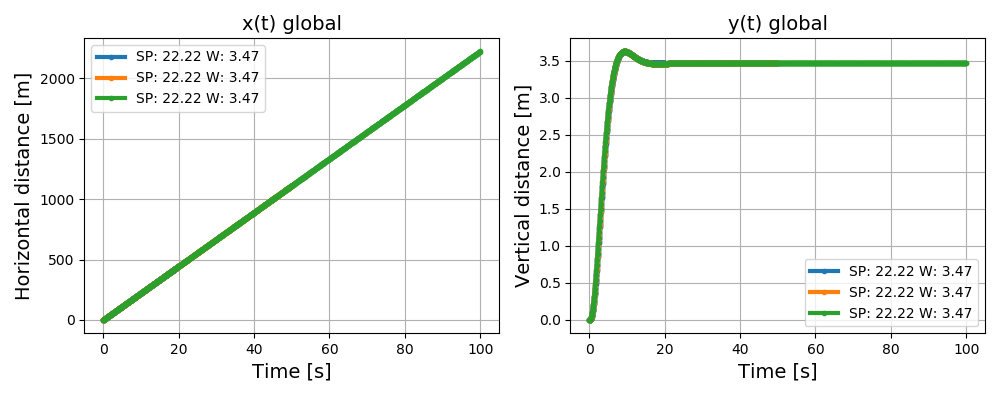
\includegraphics[width=1.0\textwidth]{1t.png}
	\label{fig:lat_acc_val}
\end{figure}


\begin{figure}[h!]
	\centering
	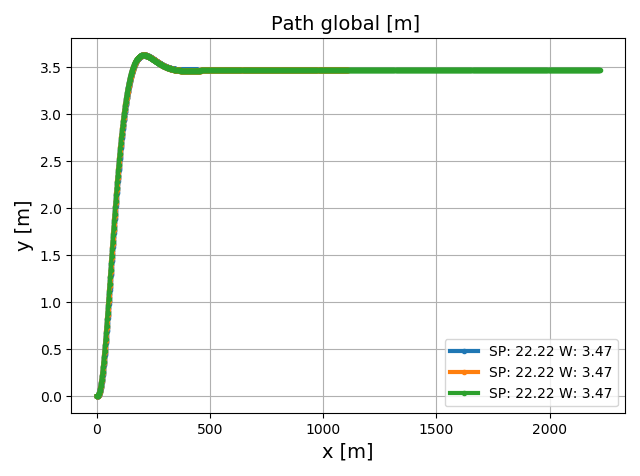
\includegraphics[width=0.8\textwidth]{2t.png}
	\label{fig:lat_acc_val}
\end{figure}

\begin{figure}[h!]
	\centering
	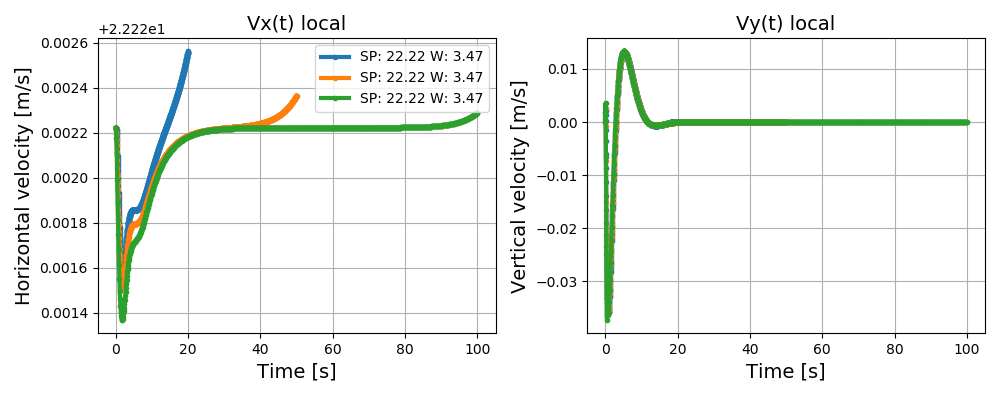
\includegraphics[width=1.0\textwidth]{3t.png}
	\label{fig:lat_acc_val}
\end{figure}


\begin{figure}[h!]
	\centering
	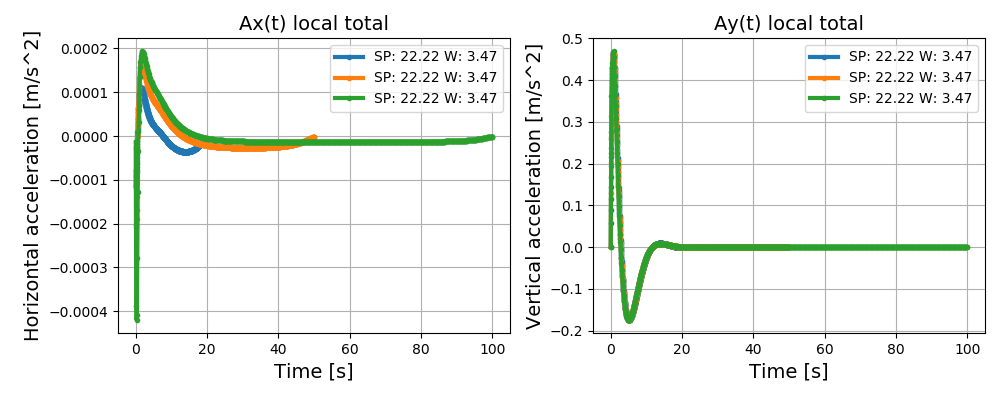
\includegraphics[width=1.0\textwidth]{4t.png}
	\label{fig:lat_acc_val}
\end{figure}


\begin{figure}[h!]
	\centering
	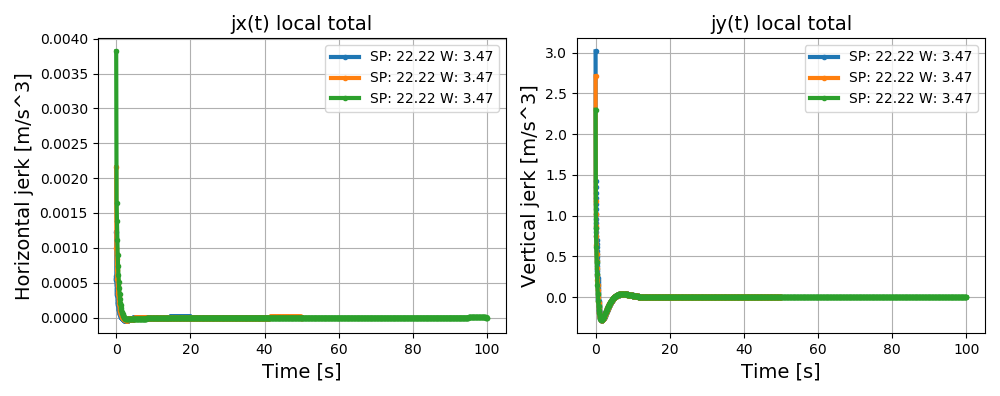
\includegraphics[width=1.0\textwidth]{5t.png}
	\label{fig:lat_acc_val}
\end{figure}


\begin{figure}[h!]
	\centering
	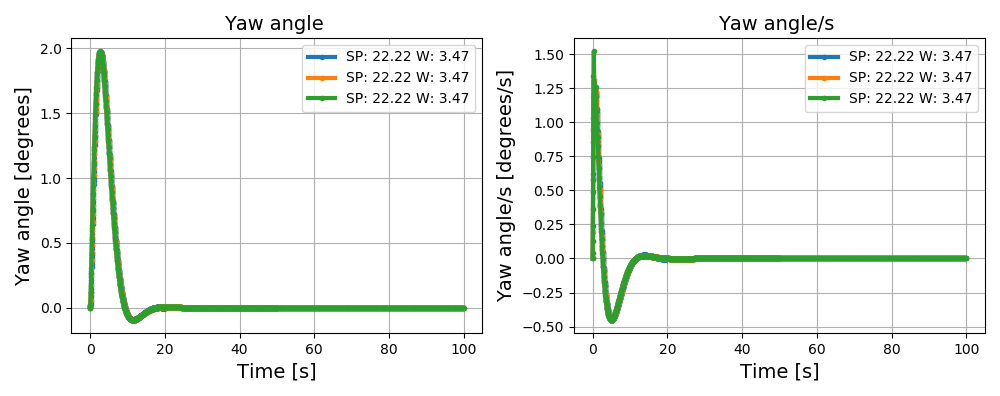
\includegraphics[width=1.0\textwidth]{6t.png}
	\label{fig:lat_acc_val}
\end{figure}


\begin{figure}[h!]
	\centering
	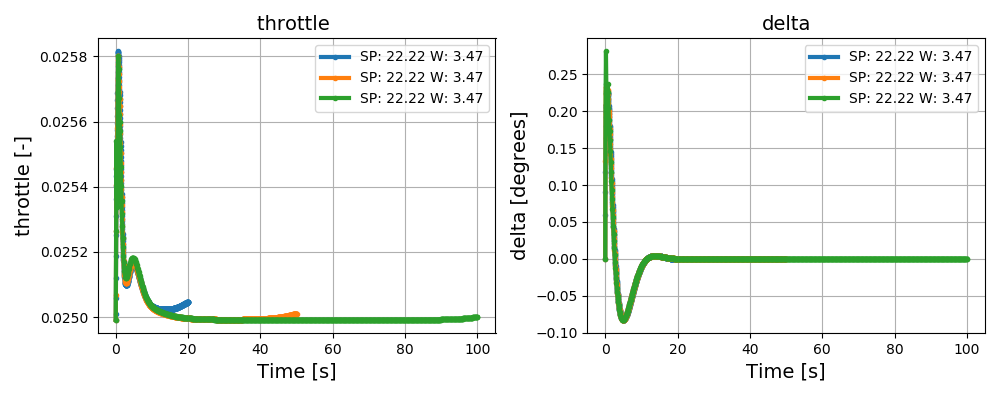
\includegraphics[width=1.0\textwidth]{7t.png}
	\label{fig:lat_acc_val}
\end{figure}


\begin{figure}[h!]
	\centering
	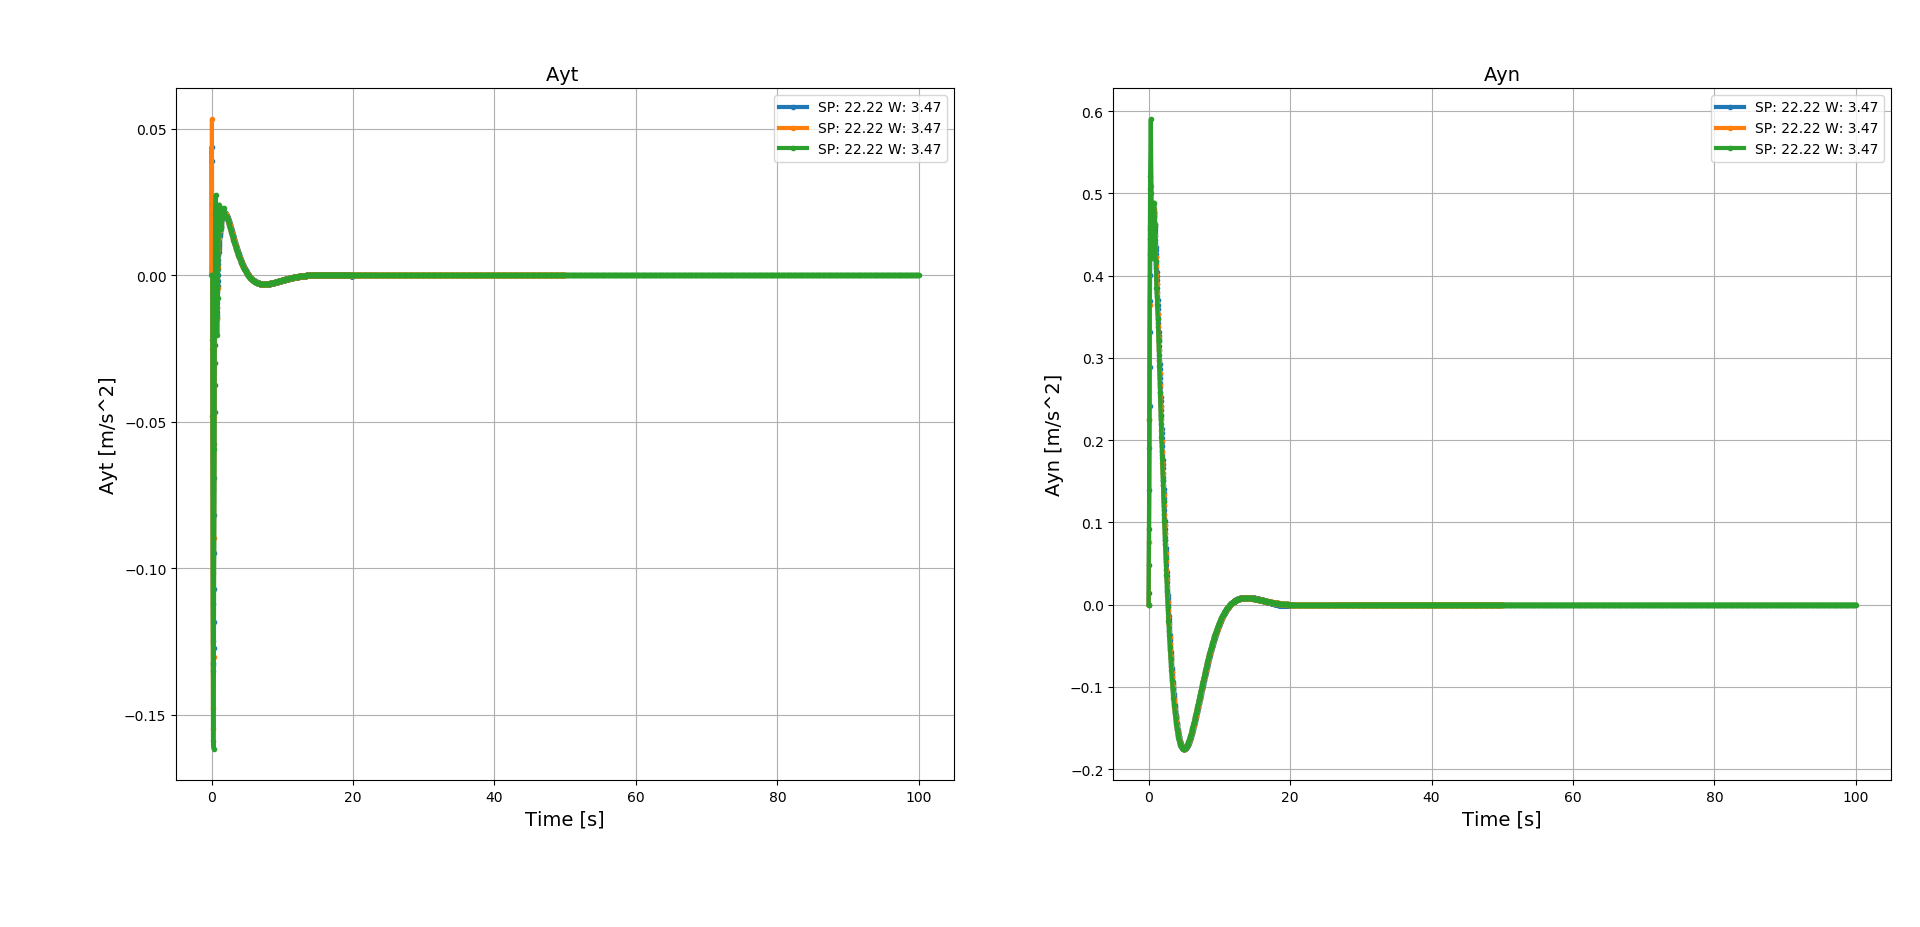
\includegraphics[width=1.0\textwidth]{8t.png}
	\label{fig:lat_acc_val}
\end{figure}


\begin{figure}[h!]
	\centering
	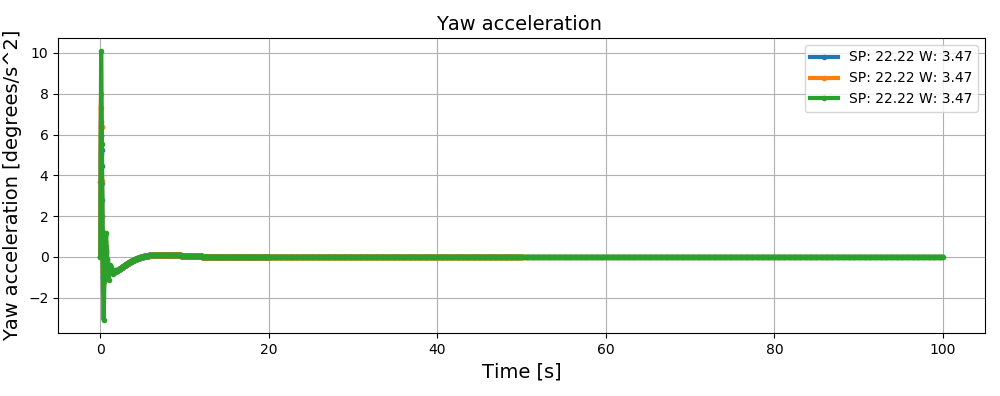
\includegraphics[width=1.0\textwidth]{9t.png}
	\label{fig:lat_acc_val}
\end{figure}


\begin{figure}[h!]
	\centering
	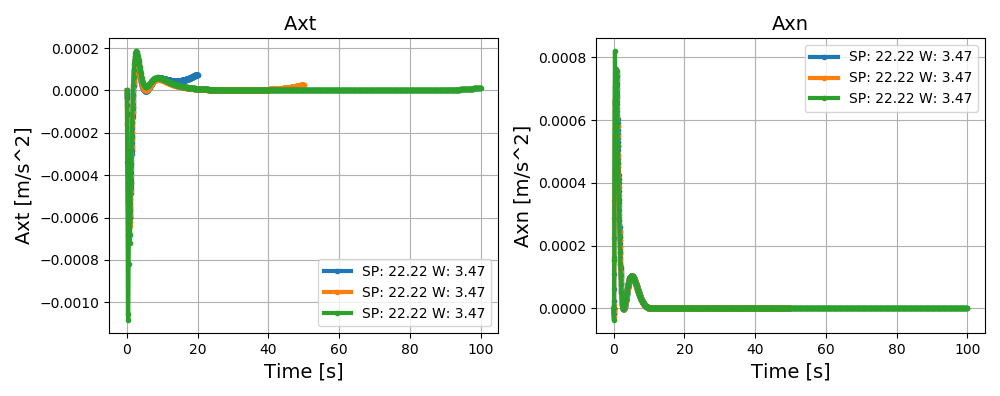
\includegraphics[width=1.0\textwidth]{10t.png}
	\label{fig:lat_acc_val}
\end{figure}


\begin{figure}[h!]
	\centering
	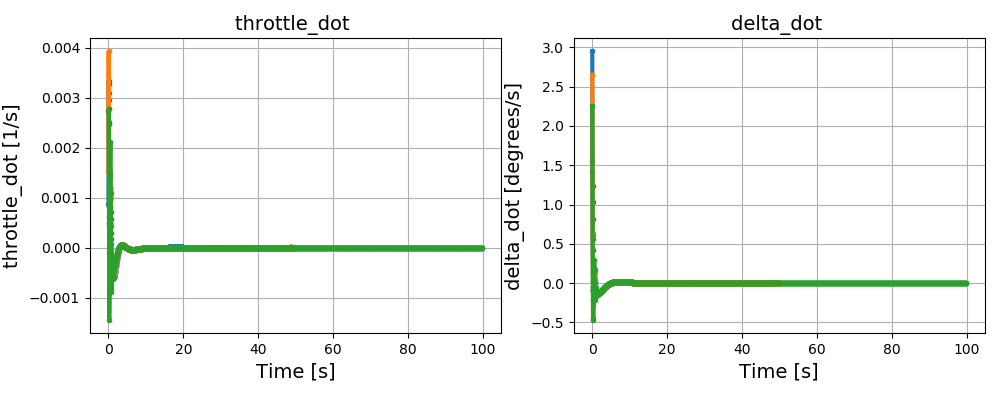
\includegraphics[width=1.0\textwidth]{11t.png}
	\label{fig:lat_acc_val}
\end{figure}


\clearpage

\section{Amount of optimization points}

 \begin{figure}[h!]
	\centering
	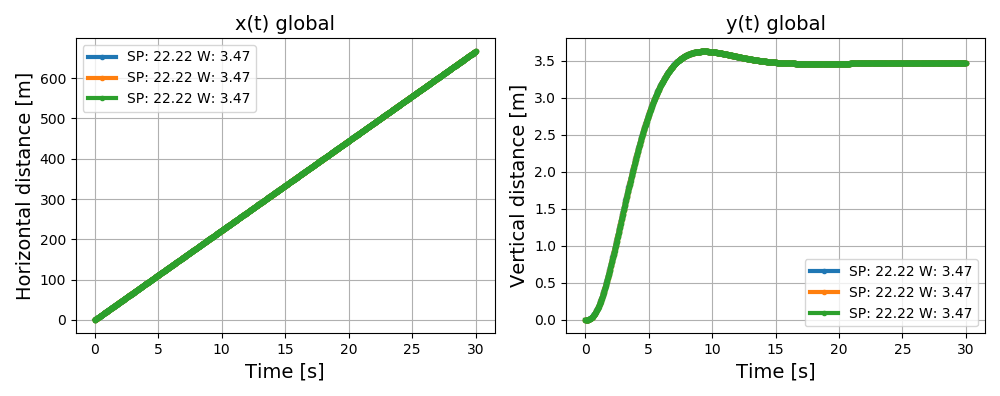
\includegraphics[width=1.0\textwidth]{1.png}
	\label{fig:lat_acc_val}
\end{figure}


\begin{figure}[h!]
	\centering
	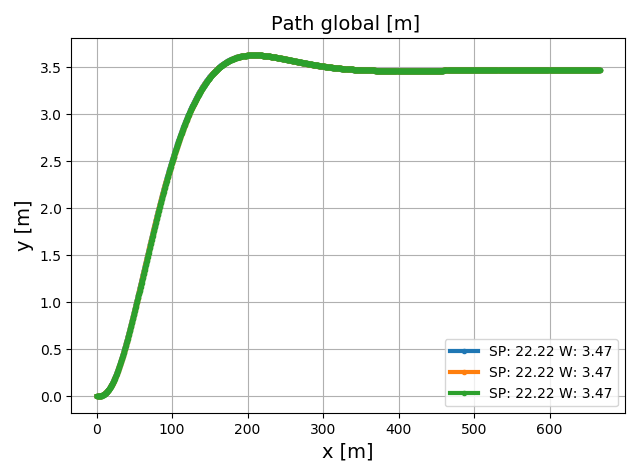
\includegraphics[width=0.8\textwidth]{2.png}
	\label{fig:lat_acc_val}
\end{figure}

\begin{figure}[h!]
	\centering
	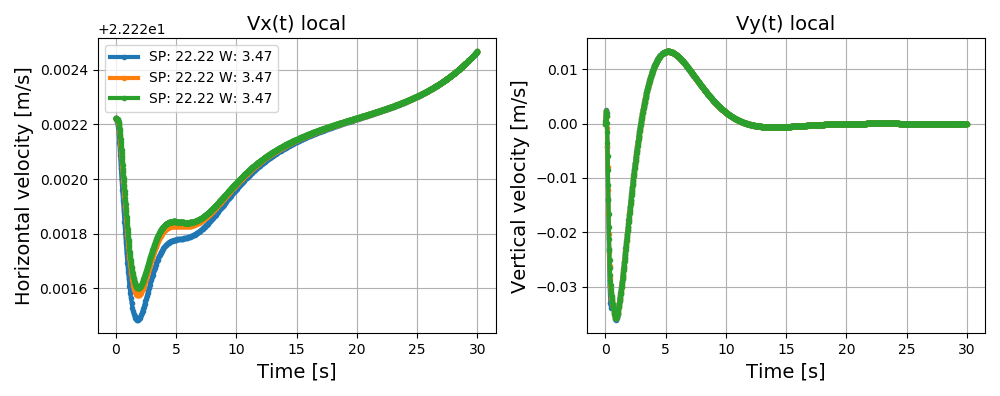
\includegraphics[width=1.0\textwidth]{3.png}
	\label{fig:lat_acc_val}
\end{figure}


\begin{figure}[h!]
	\centering
	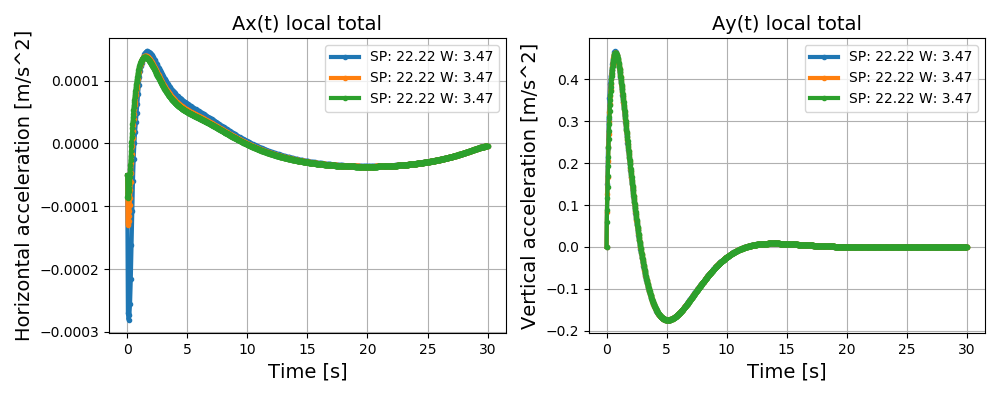
\includegraphics[width=1.0\textwidth]{4.png}
	\label{fig:lat_acc_val}
\end{figure}


\begin{figure}[h!]
	\centering
	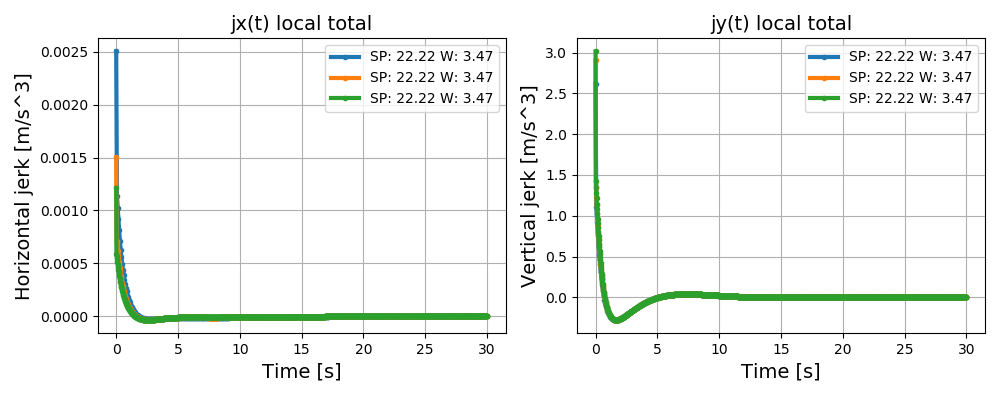
\includegraphics[width=1.0\textwidth]{5.png}
	\label{fig:lat_acc_val}
\end{figure}


\begin{figure}[h!]
	\centering
	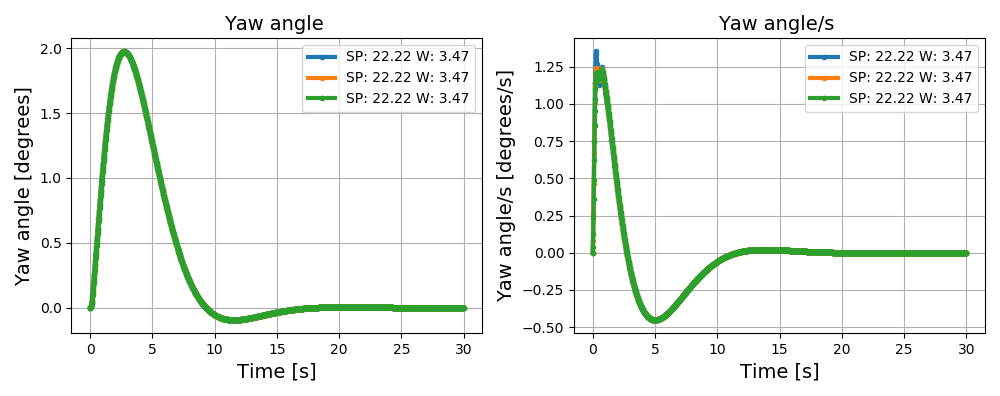
\includegraphics[width=1.0\textwidth]{6.png}
	\label{fig:lat_acc_val}
\end{figure}


\begin{figure}[h!]
	\centering
	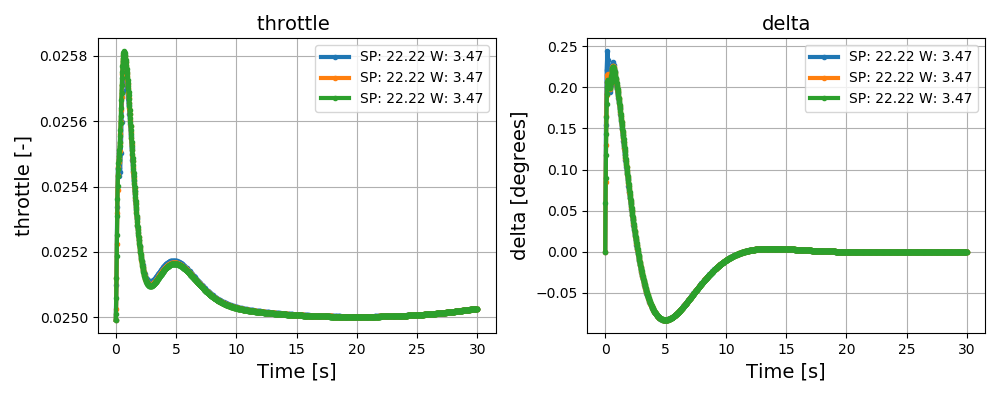
\includegraphics[width=1.0\textwidth]{7.png}
	\label{fig:lat_acc_val}
\end{figure}


\begin{figure}[h!]
	\centering
	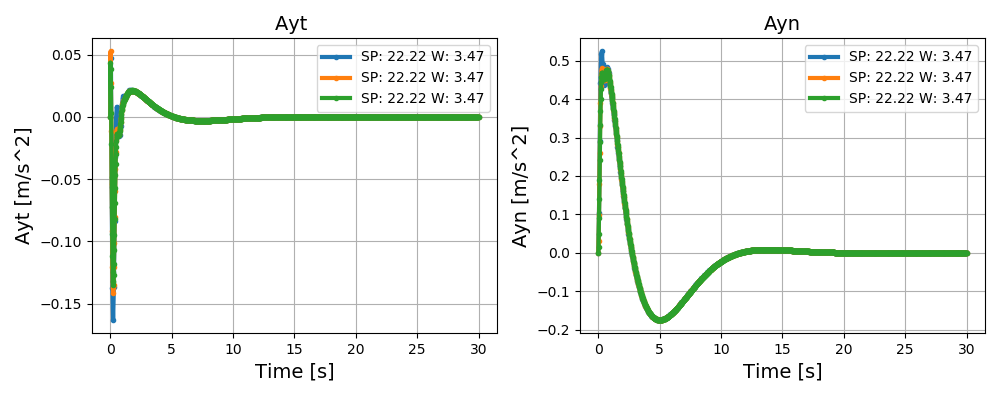
\includegraphics[width=1.0\textwidth]{8.png}
	\label{fig:lat_acc_val}
\end{figure}


\begin{figure}[h!]
	\centering
	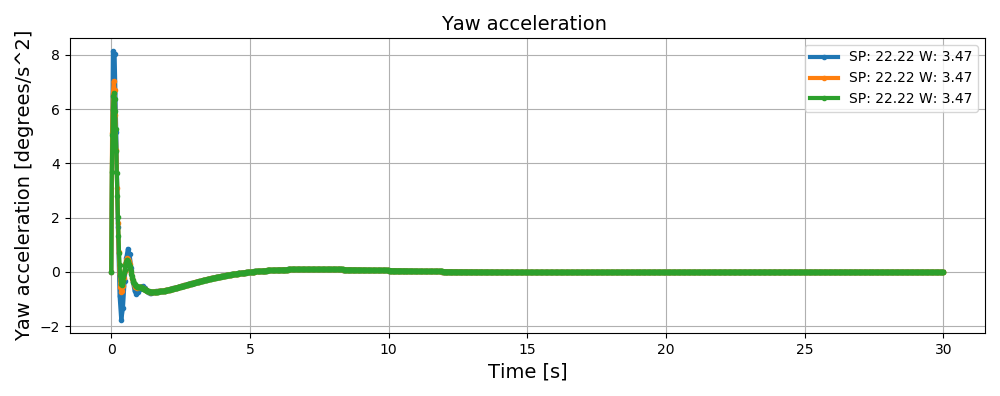
\includegraphics[width=1.0\textwidth]{9.png}
	\label{fig:lat_acc_val}
\end{figure}


\begin{figure}[h!]
	\centering
	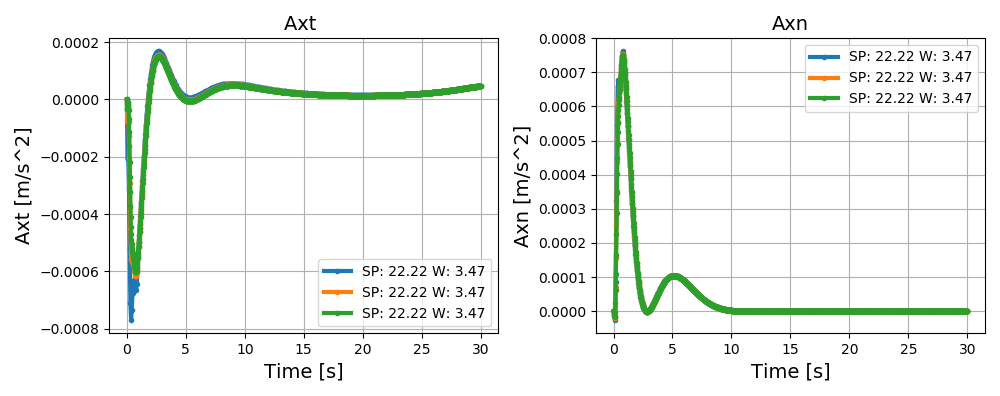
\includegraphics[width=1.0\textwidth]{10.png}
	\label{fig:lat_acc_val}
\end{figure}


\begin{figure}[h!]
	\centering
	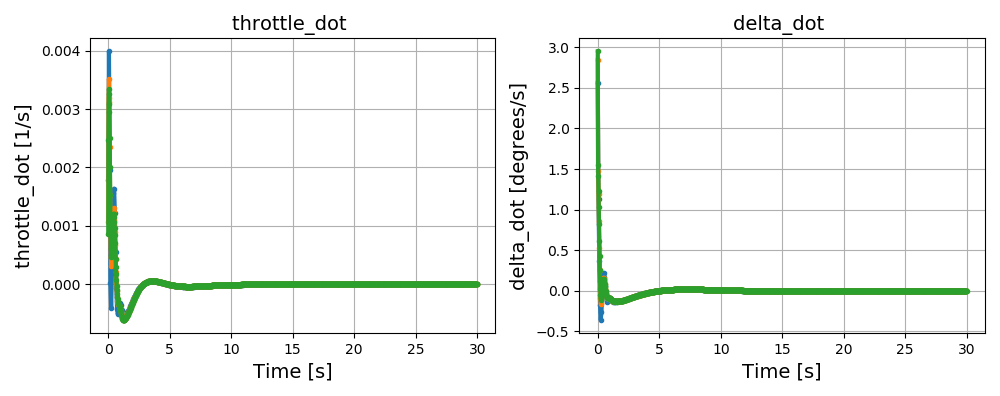
\includegraphics[width=1.0\textwidth]{11.png}
	\label{fig:lat_acc_val}
\end{figure}










%%% Local Variables: 
%%% mode: latex
%%% TeX-master: "thesis"
%%% End: 

\chapter{Results of the averaging learning on 3 datasets}
\label{app:C}
The figures shown in this appendix serve as a completion on the figures that were presented in the discussion of section \ref{s:averaging_method}. It concerns the results of the learning algorithm that learns from three ideal datasets. First the resulting kinematic signals of the bicycle model during the different lane changes are shown. It should be noted that Figure \ref{fig:app_delta} shows the angle of the front wheel of the bicycle model. In order to obtain the steerwheelangle, this relation is linearised by the factor $Gs = 16.96$ which means that $\delta_{SWA} = Gs\cdot\delta_{front}$. Further Figure \ref{fig:app_conv} displays the convergence during the learning process and plots $\bm{f}_{rel}$ over the iterations. Figure \ref{fig:app_grad} shows the absolute difference between the learned and observed features. In Figure\ref{fig:app_weights} the learning of the weights towards the final ones are presented. Figure \ref{fig:app_update} gives the difference of current weight with respect to the previous one and as last Figure \ref{fig:app_multigrad} shows which of the three RPROP cases that is used in order to update a certain weight. 

 
\begin{figure}[h!]
	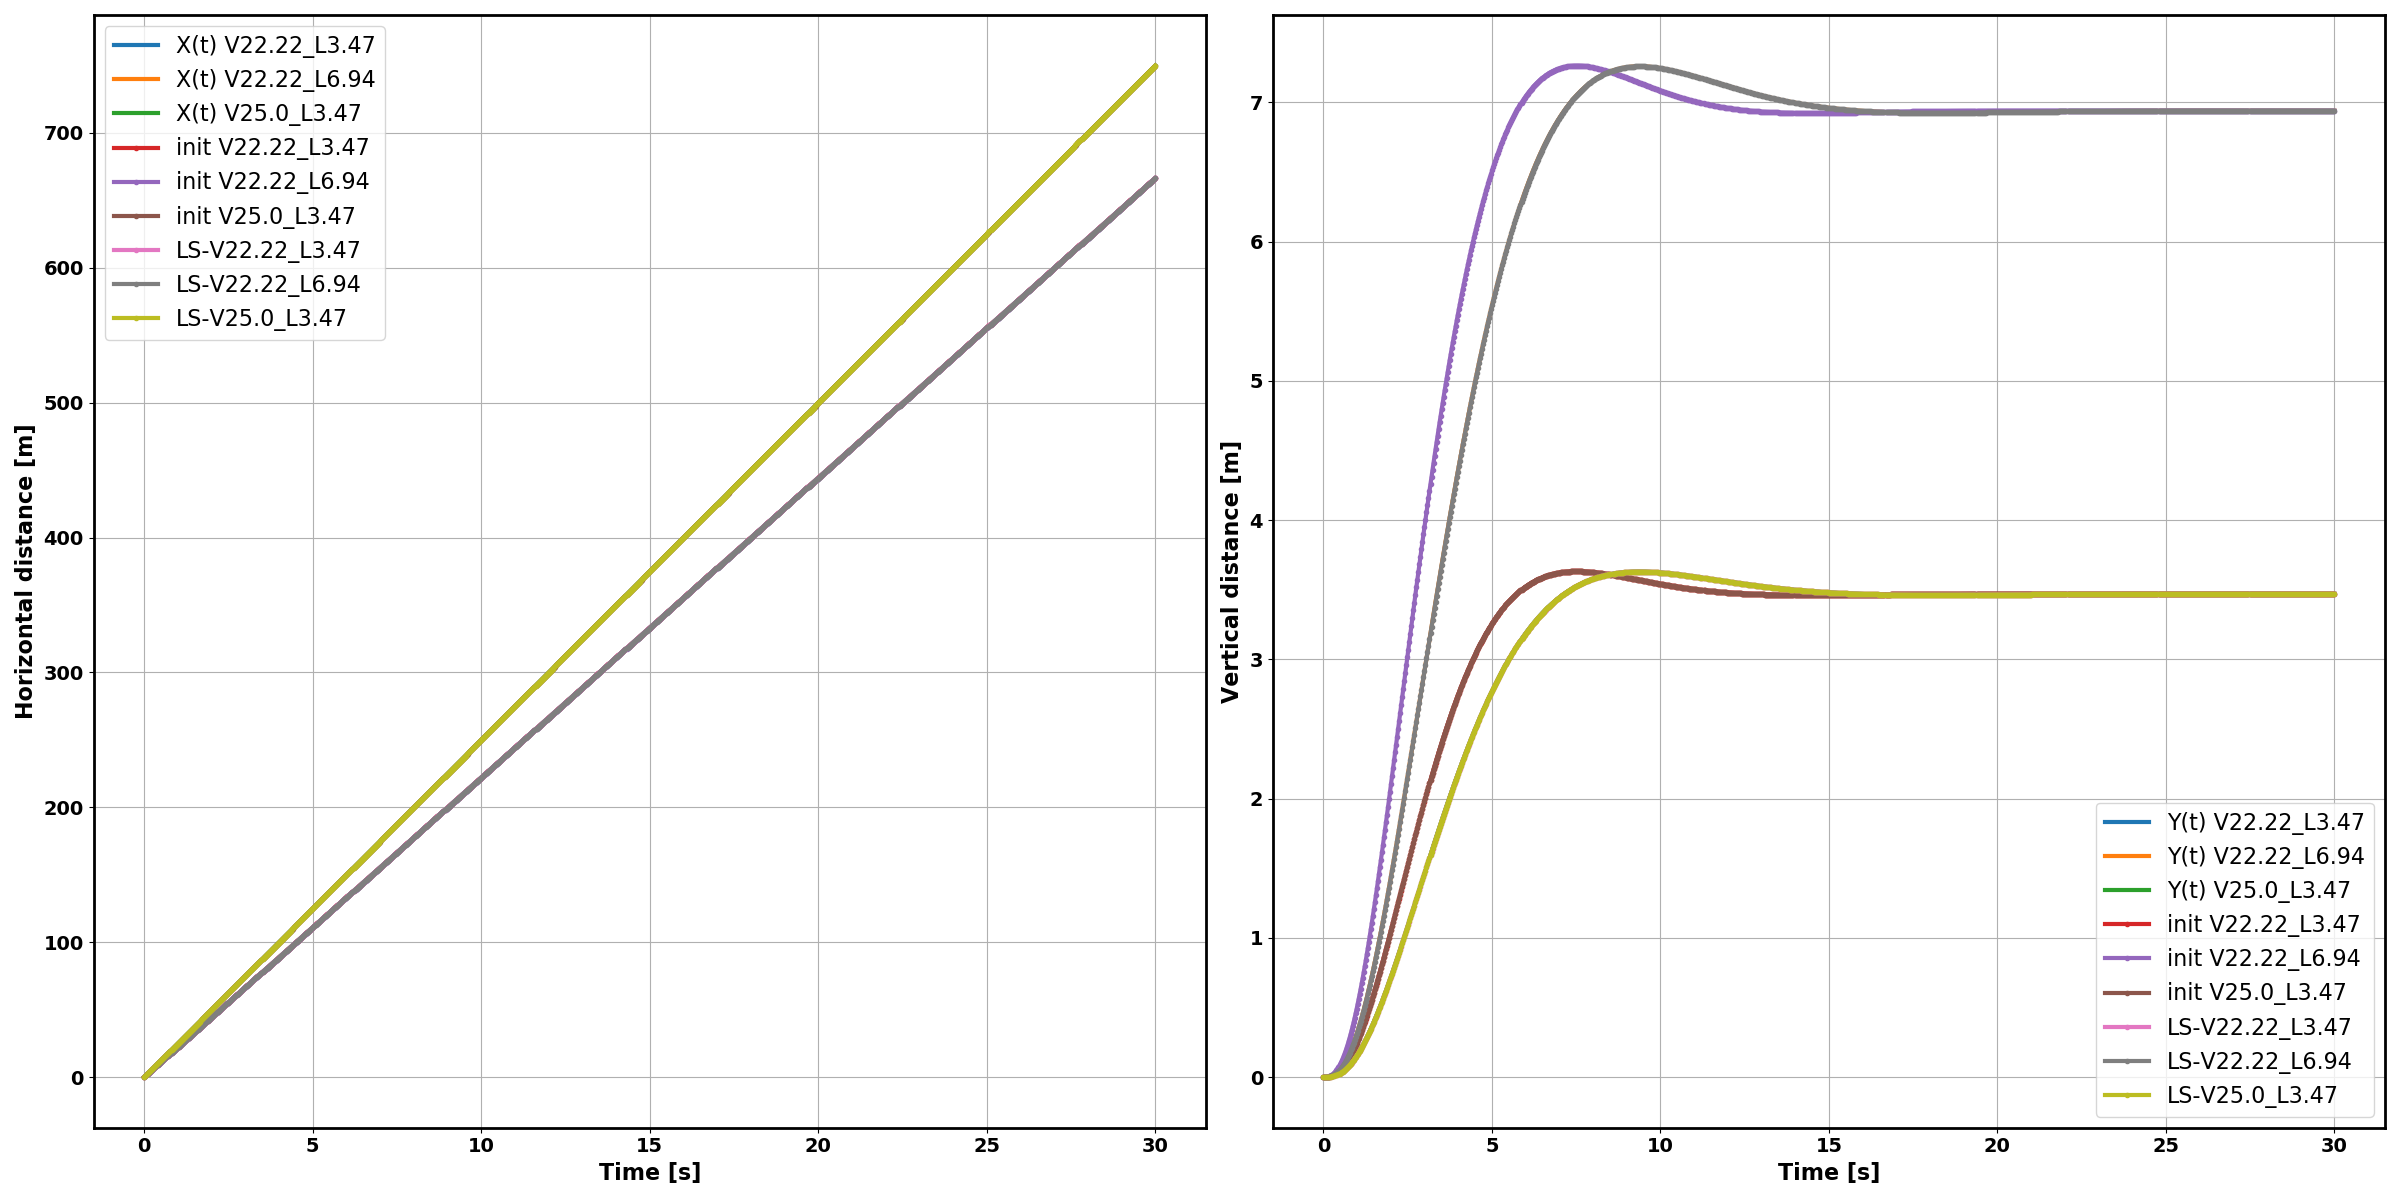
\includegraphics[width=1.0\textwidth]{1l.png}
\end{figure}

\begin{figure}[h!]
	\centering
	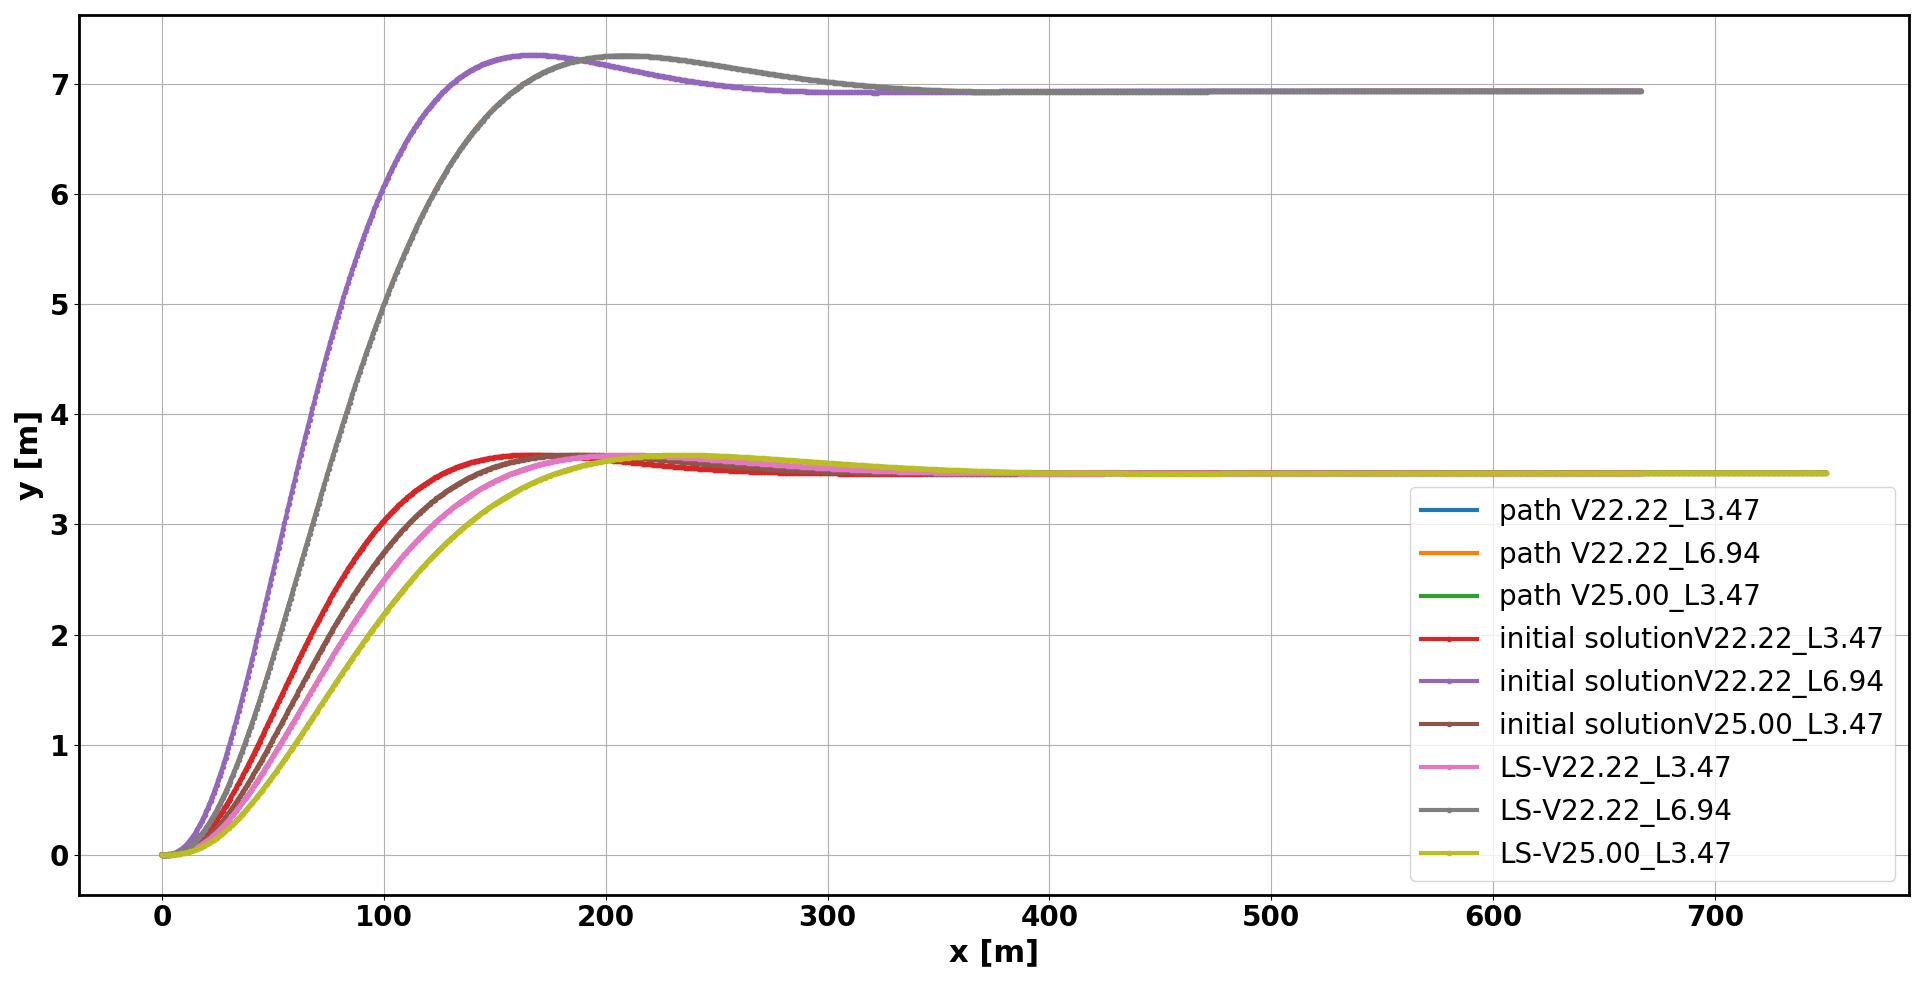
\includegraphics[width=1.0\textwidth]{2l.png}
	\label{fig:lat_acc_val}
\end{figure}

\begin{figure}[h!]
	\centering
	\includegraphics[width=1.0\textwidth]{3l.png}
	\label{fig:lat_acc_val}
\end{figure}


\begin{figure}[h!]
	\centering
	\includegraphics[width=1.0\textwidth]{4l.png}
	\label{fig:lat_acc_val}
\end{figure}


\begin{figure}[h!]
	\centering
	\includegraphics[width=1.0\textwidth]{5l.png}
	\label{fig:lat_acc_val}
\end{figure}


\begin{figure}[h!]
	\centering
	\includegraphics[width=1.0\textwidth]{6l.png}
	\label{fig:lat_acc_val}
\end{figure}


\begin{figure}[h!]
	\centering
	\includegraphics[width=1.0\textwidth]{7l.png}
	\caption{This figure shows the amount of throttle and the angle of the front wheel of the bicycle model during the lane change maneuvers.}
	\label{fig:app_delta}
\end{figure}


\begin{figure}[h!]
	\centering
	\includegraphics[width=1.0\textwidth]{8l.png}
	\label{fig:lat_acc_val}
\end{figure}


\begin{figure}[h!]
	\centering
	\includegraphics[width=1.0\textwidth]{9l.png}
	\label{fig:lat_acc_val}
\end{figure}


\begin{figure}[h!]
	\centering
	\includegraphics[width=1.0\textwidth]{10l.png}
	\label{fig:lat_acc_val}
\end{figure}


\begin{figure}[h!]
	\centering
	\includegraphics[width=1.0\textwidth]{11l.png}
	\label{fig:lat_acc_val}
\end{figure}



\begin{figure}[h!]
	\centering
	\includegraphics[width=1.0\textwidth]{12l.png}	
	\caption{The convergence of $\bm{f}_{rel}$ towards one during the learning iterations.}
	\label{fig:app_conv}
\end{figure}


\begin{figure}[h!]
	\centering
	\includegraphics[width=1.0\textwidth]{13l.png}
	\caption{The gradient $\pdv{\bm{F}}{\bm{\theta}}$ estimated by $\bm{F}_{obs} - \bm{F}(\bm{r}_{expected})$ towards zero during the different learning iterations. }
	\label{fig:app_grad}
\end{figure}

\begin{figure}[h!]
	\centering
	\includegraphics[width=1.0\textwidth]{14l.png}
	\caption{The learned weights during the different learning iterations.}
	\label{fig:app_weights}
	
\end{figure}


\begin{figure}[h!]
	\centering
	\includegraphics[width=1.0\textwidth]{15l.png}
	\caption{The difference of $\bm{\theta}$ with respect to one used in the previous iteration. }
	\label{fig:app_update}
\end{figure}


\begin{figure}[h!]
	\centering
	\includegraphics[width=1.0\textwidth]{16l.png}
	\caption{This figure shows which case of the three available in the RPROP algorithm is chosen during the learning iterations.}
	\label{fig:app_multigrad}
\end{figure}












%%% Local Variables: 
%%% mode: latex
%%% TeX-master: "thesis"
%%% End: 

\chapter{Accuracy results of the tracking MPC}
\label{app:D}
This appendix shows the results that are discussed in \ref{s:tracking_results}. In red the reference is shown that was derived from \ref{opt:basic_opti_w} with using the bicycle model and in blue the trajectory completed by the Amesim model. During the learning process with the Amesim model (section \ref{s:complex_learning_results}) the first $10 \hspace{1mm}s$ of the Amesim trajectory is thrown away in order to remove the unstable longitudinal behaviour at the start of the simulation.


\begin{figure}[h!]
	\centering
	\includegraphics[width=1.15\textwidth]{1path_N50_TMPC C0.1_Tf40.PNG}
\end{figure}

\begin{figure}[h!]
	\centering
	\includegraphics[width=1.15\textwidth]{2xy_N50_TMPC 0.1_Tf40.PNG}
\end{figure}

\begin{figure}[h!]
	\centering
	\includegraphics[width=1.15\textwidth]{3vxy_N50_TMPC 0.1_Tf40.PNG}
\end{figure}


\begin{figure}[h!]
	\centering
	\includegraphics[width=1.15\textwidth]{6atot_N50_TMPC 0.1_Tf40.PNG}
\end{figure}


\begin{figure}[h!]
	\centering
	\includegraphics[width=1.15\textwidth]{5ax_N50_TMPC 0.1_Tf40.PNG}
\end{figure}

\begin{figure}[h!]
	\centering
	\includegraphics[width=1.15\textwidth]{4ay_N50_TMPC 0.1_Tf40.PNG}
\end{figure}

\begin{figure}[h!]
	\centering
	\includegraphics[width=1.15\textwidth]{7psi_N50_TMPC 0.1_Tf40.PNG}
\end{figure}

\begin{figure}[h!]
	\centering
	\includegraphics[width=1.15\textwidth]{8tr&delta_N50_TMPC 0.1_Tf40.PNG}
\end{figure}

\begin{figure}[h!]
	\centering
	\includegraphics[width=1.15\textwidth]{9jerks_N50_TMPC 0.1_Tf40.PNG}
\end{figure}

\begin{figure}[h!]
	\centering
	\includegraphics[width=1.15\textwidth]{14tr_dot&delta_dot_N50_TMPC 0.1_Tf40.PNG}
\end{figure}














%%% Local Variables: 
%%% mode: latex
%%% TeX-master: "thesis"
%%% End: 

\chapter{Results of learning with the 15 dof Amesim model}
\label{app:E}
This appendix shows the learning results of the 15 dof Amesim model on two distinct as possible datasets $V022.22 - L3.47$ and $V025.00 - L6.94$. Except for the longitudinal total acceleration and jerk, all the learned kinematic signals match closely with the observed one. The most important conclusions about the results can be find in section \ref{s:complex_learning_results}.\\
It should be noted that Figure \ref{fig:app_deltaE} and \ref{fig:app_delta_dotE}  show the angle of the front wheel of the bicycle model. In order to obtain the steerwheelangle, this relation is linearised by the factor $Gs = 16.96$ which means that $\delta_{SWA} = Gs\cdot\delta_{front}$. Further Figure \ref{fig:app_convE} displays the convergence during the learning process and plots $\bm{f}_{rel}$ over the iterations. Figure \ref{fig:app_gradE} shows the absolute difference between the learned and observed features. In Figure\ref{fig:app_weightsE} the learning of the weights towards the final ones are presented. Figure \ref{fig:app_updateE} gives the difference of current weight with respect to the previous one and as last Figure \ref{fig:app_multigradE} shows which of the three RPROP cases that is used in order to update a certain weight.



\begin{figure}[h!]
	\centering
	\includegraphics[width=1.15\textwidth]{2path_N1000IT28.PNG}
\end{figure}

\begin{figure}[h!]
	\centering
	\includegraphics[width=1.15\textwidth]{1X_Y_N1000IT28.PNG}
\end{figure}


\begin{figure}[h!]
	\centering
	\includegraphics[width=1.15\textwidth]{3VX_VY_N1000IT28.PNG}
\end{figure}


\begin{figure}[h!]
	\centering
	\includegraphics[width=1.15\textwidth]{4AX_AY_N1000IT28.PNG}
\end{figure}


\begin{figure}[h!]
	\centering
	\includegraphics[width=1.15\textwidth]{5AtX_AnX_N1000IT28.PNG}
\end{figure}

\begin{figure}[h!]
	\centering
	\includegraphics[width=1.15\textwidth]{6AtY_AnY_N1000IT28.PNG}
\end{figure}

\begin{figure}[h!]
	\centering
	\includegraphics[width=1.15\textwidth]{7JX_JY_N1000IT28.PNG}
\end{figure}

\begin{figure}[h!]
	\centering
	\includegraphics[width=1.15\textwidth]{8yaws_N1000IT28.PNG}
\end{figure}

\begin{figure}[h!]
	\centering
	\includegraphics[width=1.15\textwidth]{9yawacc_N1000IT28.PNG}
\end{figure}

\begin{figure}[h!]
	\centering
	\includegraphics[width=1.15\textwidth]{10trdelta_N1000IT28.PNG}
	\caption{This figure shows the amount of throttle and the angle of the front wheel of the bicycle model during the lane change maneuvers.}
	\label{fig:app_deltaE}
\end{figure}

\begin{figure}[h!]
	\centering
	\includegraphics[width=1.15\textwidth]{11trdelta_dot_N1000IT28.PNG}
	\caption{This figure shows the amount of first derivative of throttle and the first derivative of the angle of the front wheel of the bicycle model is given as input during the lane change maneuvers.}
	\label{fig:app_delta_dotE}
\end{figure}

\begin{figure}[h!]
	\centering
	\includegraphics[width=1.15\textwidth]{12frel.PNG}
	\caption{The convergence of $\bm{f}_{rel}$ towards one during the learning iterations.}
	\label{fig:app_convE}
\end{figure}

\begin{figure}[h!]
	\centering
	\includegraphics[width=1.15\textwidth]{13gradcurr.PNG}
	\caption{The gradient $\pdv{\bm{F}}{\bm{\theta}}$ estimated by $\bm{F}_{obs} - \bm{F}(\bm{r}_{expected})$ towards zero during the different learning iterations. }
	\label{fig:app_gradE}
\end{figure}

\begin{figure}[h!]
	\centering
	\includegraphics[width=1.15\textwidth]{14weights.PNG}
	\caption{The learned weights during the different learning iterations.}
	\label{fig:app_weightsE}
\end{figure}

\begin{figure}[h!]
	\centering
	\includegraphics[width=1.15\textwidth]{15updateweights.PNG}
	\caption{The difference of $\bm{\theta}$ with respect to one used in the previous iteration. }
	\label{fig:app_updateE}
\end{figure}

\begin{figure}[h!]
	\centering
	\includegraphics[width=1.15\textwidth]{16multigrad.PNG}
	\caption{This figure shows which case of the three available in the RPROP algorithm is chosen during the learning iterations.}
	\label{fig:app_multigradE}
\end{figure}





%%% Local Variables: 
%%% mode: latex
%%% TeX-master: "thesis"
%%% End: 


\backmatter
% Na de bijlagen plaatst men nog de bibliografie.
% Je kan de  standaard "abbrv" bibliografiestijl vervangen door een andere.
\bibliographystyle{abbrv}
\bibliography{Thesis_ref}
%\bibliography{references}

\end{document}

%%% Local Variables: 
%%% mode: latex
%%% TeX-master: t
%%% End: 
